\documentclass[a4paper,12pt]{report}
\usepackage{inputenc}
\usepackage[T1]{fontenc}
\usepackage[french, arabic]{babel} % If you write in French
\usepackage{a4wide}
\usepackage[framed,numbered,autolinebreaks,useliterate]{mcode}
\usepackage{graphicx}
\usepackage{placeins}
%pour la mise en page des tableaux
\usepackage{array}
\usepackage{tabularx}
\usepackage{xcolor}
\definecolor{darkgrey}{RGB}{45,45,45}
\definecolor{yellow}{RGB}{255,193,7}
\usepackage{longtable}
\usepackage{float}
\usepackage{array} % for extrarowheight
\usepackage{lscape}
\usepackage{afterpage}
\usepackage{rotating}
\usepackage[nottoc,notlof,notlot]{tocbibind}
\usepackage{tocloft}
\usepackage{pdfpages}
\usepackage{microtype}

\graphicspath{{images/}{images_pfe/}}
\newlength\figureheight
\newlength\figurewidth
\usepackage{ifthen}
\usepackage{ifpdf}

\usepackage{hyperref}
\hypersetup{%
colorlinks=true,
linkcolor=blue,
citecolor=green,
urlcolor=blue}
% \urlstyle{same}
\usepackage{standalone}
\usepackage{import}









\usepackage[top=2.5cm,bottom=2.5cm,right=2.5cm,left=2.5cm]{geometry}
\usepackage{changepage}
\usepackage{tikz}
\definecolor{Gray}{gray}{0.9}
\definecolor{LightCyan}{rgb}{0.88,1,1}
\usetikzlibrary{matrix,fit,backgrounds,arrows,shapes,positioning,shadows,trees,quotes}


\tikzset{
  basic/.style  = {draw, text width=2cm, drop shadow, font=\sffamily, rectangle},
  root/.style   = {basic, rounded corners=2pt, thin, align=center,
                   fill=yellow!30},
  level 2/.style = {basic, rounded corners=6pt, thin,align=center, fill=green!40,
                   text width=8em},
  level 3/.style = {basic, thin, align=left, fill=blue!25, text width=6.5em},
  level 4/.style = {basic, ellipse, thin , align=center, fill=pink!40, text width = 4em},
}
\usepackage{tabularx}
    \newcolumntype{L}{>{\raggedright\arraybackslash}X}
\usepackage{longtable}

\usepackage{xltabular}
\renewcommand{\tablename}{Tableau}
\renewcommand{\figurename}{Figure}



%pour les références bibliographiques
\usepackage{cite}

%% pour la numération des sous sou sections



% pour les algorithmes
\usepackage[ruled,vlined,linesnumbered]{algorithm2e}
\DontPrintSemicolon

\setlength\arrayrulewidth{1pt}
\renewcommand{\baselinestretch}{1.05}
\usepackage{fancyhdr}
\pagestyle{fancy}
\fancyhf{}
\lhead{\bfseries\nouppercase{\leftmark}}
\rfoot{\bfseries\thepage}
\setlength{\headheight}{14.5pt}

\let\headruleORIG\headrule

\renewcommand{\headrule}{\color{black} \headruleORIG}
\renewcommand{\headrulewidth}{1.0pt}
\usepackage{colortbl}
\arrayrulecolor{black}

\fancypagestyle{plain}{
  \fancyhead{}
  \fancyfoot[R]{\bfseries\thepage}
  \renewcommand{\headrulewidth}{0pt}
}



\makeatletter
\def\@textbottom{\vskip \z@ \@plus 1pt}
\let\@texttop\relax
\makeatother

\makeatletter
\def\cleardoublepage{\clearpage\if@twoside \ifodd\c@page\else%
  \hbox{}%
  \thispagestyle{empty}%
  \newpage%
  \if@twocolumn\hbox{}\newpage\fi\fi\fi}
\makeatother
\usepackage{amsmath}
\usepackage{amssymb}
\usepackage{bbm}
\usepackage{array}
\usepackage{bm}
\usepackage{multirow}
\usepackage[footnote]{acronym}

\usepackage[bottom]{footmisc}

\usepackage{listings}

\lstdefinestyle{vscode}{
  basicstyle=\ttfamily\small,
  backgroundcolor=\color{white},
  keywordstyle=\color{yellow},
  commentstyle=\color{green!50!black},
  stringstyle=\color{orange},
  identifierstyle=\color{black},
  numbers=left,
  numberstyle=\tiny\color{black},
  tabsize=2,
  frame=single,
  rulecolor=\color{lightgray},
  breaklines=true,
  showstringspaces=false,
  captionpos=b,
  extendedchars=true,
  aboveskip=1em,
  belowskip=1em,
  xleftmargin=1em,
  framexleftmargin=1em,
  escapeinside={(*@}{@*)},
  language=Python,
  literate=
    {*}{{\textcolor{blue}{*}}}1
    {-}{{\textcolor{blue}{-}}}1
    {+}{{\textcolor{blue}{+}}}1
    {/}{{\textcolor{blue}{/}}}1
    {=}{{\textcolor{blue}{=}}}1
    {>}{{\textcolor{blue}{>}}}1
    {<}{{\textcolor{blue}{<}}}1
    {;}{{\textcolor{blue}{;}}}1
    {,}{{\textcolor{blue}{,}}}1
    {\{}{{\textcolor{blue}{\{}}}1
    {\}}{{\textcolor{blue}{\}}}}1
    {[}{{\textcolor{blue}{[}}}1
    {]}{{\textcolor{blue}{]}}}1
    {(}{{\textcolor{blue}{(}}}1
    {)}{{\textcolor{blue}{)}}}1
}
%table break line

\usepackage{makecell}
\usepackage{xcolor,colortbl}

\renewcommand\theadalign{bl}
\renewcommand\theadfont{\bfseries}
\renewcommand\cellalign{bl}
\renewcommand\cellgape{\Gape[2pt]}

\parskip=5pt
%\sloppy
 %%%%********************************************************************
\definecolor{quotemark}{gray}{0.7}
\makeatletter
\def\fquote{%
    \@ifnextchar[{\fquote@i}{\fquote@i[]}%]
           }%
\def\fquote@i[#1]{%
    \def\tempa{#1}%
    \@ifnextchar[{\fquote@ii}{\fquote@ii[]}%]
                 }%
\def\fquote@ii[#1]{%
    \def\tempb{#1}%
    \@ifnextchar[{\fquote@iii}{\fquote@iii[]}%]
                      }%
\def\fquote@iii[#1]{%
    \def\tempc{#1}%
    \vspace{1em}%
    \noindent%
    \begin{list}{}{%
         \setlength{\leftmargin}{0.1\textwidth}%
         \setlength{\rightmargin}{0.1\textwidth}%
                  }%
         \item[]%
         \begin{picture}(0,0)%
         \put(-15,-5){\makebox(0,0){\scalebox{3}{\textcolor{quotemark}{``}}}}%
         \end{picture}%
         \begingroup\itshape}%
 %%%%********************************************************************
 \def\endfquote{%
 \endgroup\par%
 \makebox[0pt][l]{%
 \hspace{0.8\textwidth}%
 \begin{picture}(0,0)(0,0)%
 \put(15,15){\makebox(0,0){%
 \scalebox{3}{\color{quotemark}''}}}%
 \end{picture}}%
 \ifx\tempa\empty%
 \else%
    \ifx\tempc\empty%
       \hfill\rule{100pt}{0.5pt}\\\mbox{}\hfill\tempa,\ \emph{\tempb}%
   \else%
       \hfill\rule{100pt}{0.5pt}\\\mbox{}\hfill\tempa,\ \emph{\tempb},\ \tempc%
   \fi\fi\par%
   \vspace{0.5em}%
 \end{list}%
 }%
 \makeatother
 %%%%********************************************************************

 \usepackage{afterpage}

\newcommand\blankpage{%
    \null
    \thispagestyle{empty}%
    \addtocounter{page}{-1}%
    \newpage}
    
\renewcommand{\listalgorithmcfname}{Liste des algorithmes}
\usepackage{polyglossia}
\setmainlanguage{french}
\setotherlanguage{arabic}
\newfontfamily\arabicfont[Script=Arabic,Scale=1]{Amiri}

\newcommand{\mychapter}[2]{
    
    \chapter*{#2}
    \addcontentsline{toc}{chapter}{#2}
}

\usepackage[page,toc,titletoc,title]{appendix}

\addto\captionsfrench{%
  \renewcommand\appendixname{Annexe}
  \renewcommand\appendixpagename{Annexes}
  \renewcommand{\appendixtocname}{Annexes}
}
\usepackage{etoolbox}
\appto\appendix{\addtocontents{toc}{\protect\setcounter{tocdepth}{0}}}

% reinstate the correct level for list of tables and figures and algorithms
\appto\listoffigures{\addtocontents{lof}{\protect\setcounter{tocdepth}{1}}}
\appto\listoftables{\addtocontents{lot}{\protect\setcounter{tocdepth}{1}}}
\appto\listofalgorithms{\addtocontents{loa}{\protect\setcounter{tocdepth}{1}}}
\usepackage{booktabs} % Add this line

\usepackage{pifont}
\usepackage{graphicx}
\begin{document}


% \includepdf[pages=-]{images_pfe/00-Page-de-garde-Mouhcine.pdf}
\import{./}{00-Page-de-garde}

%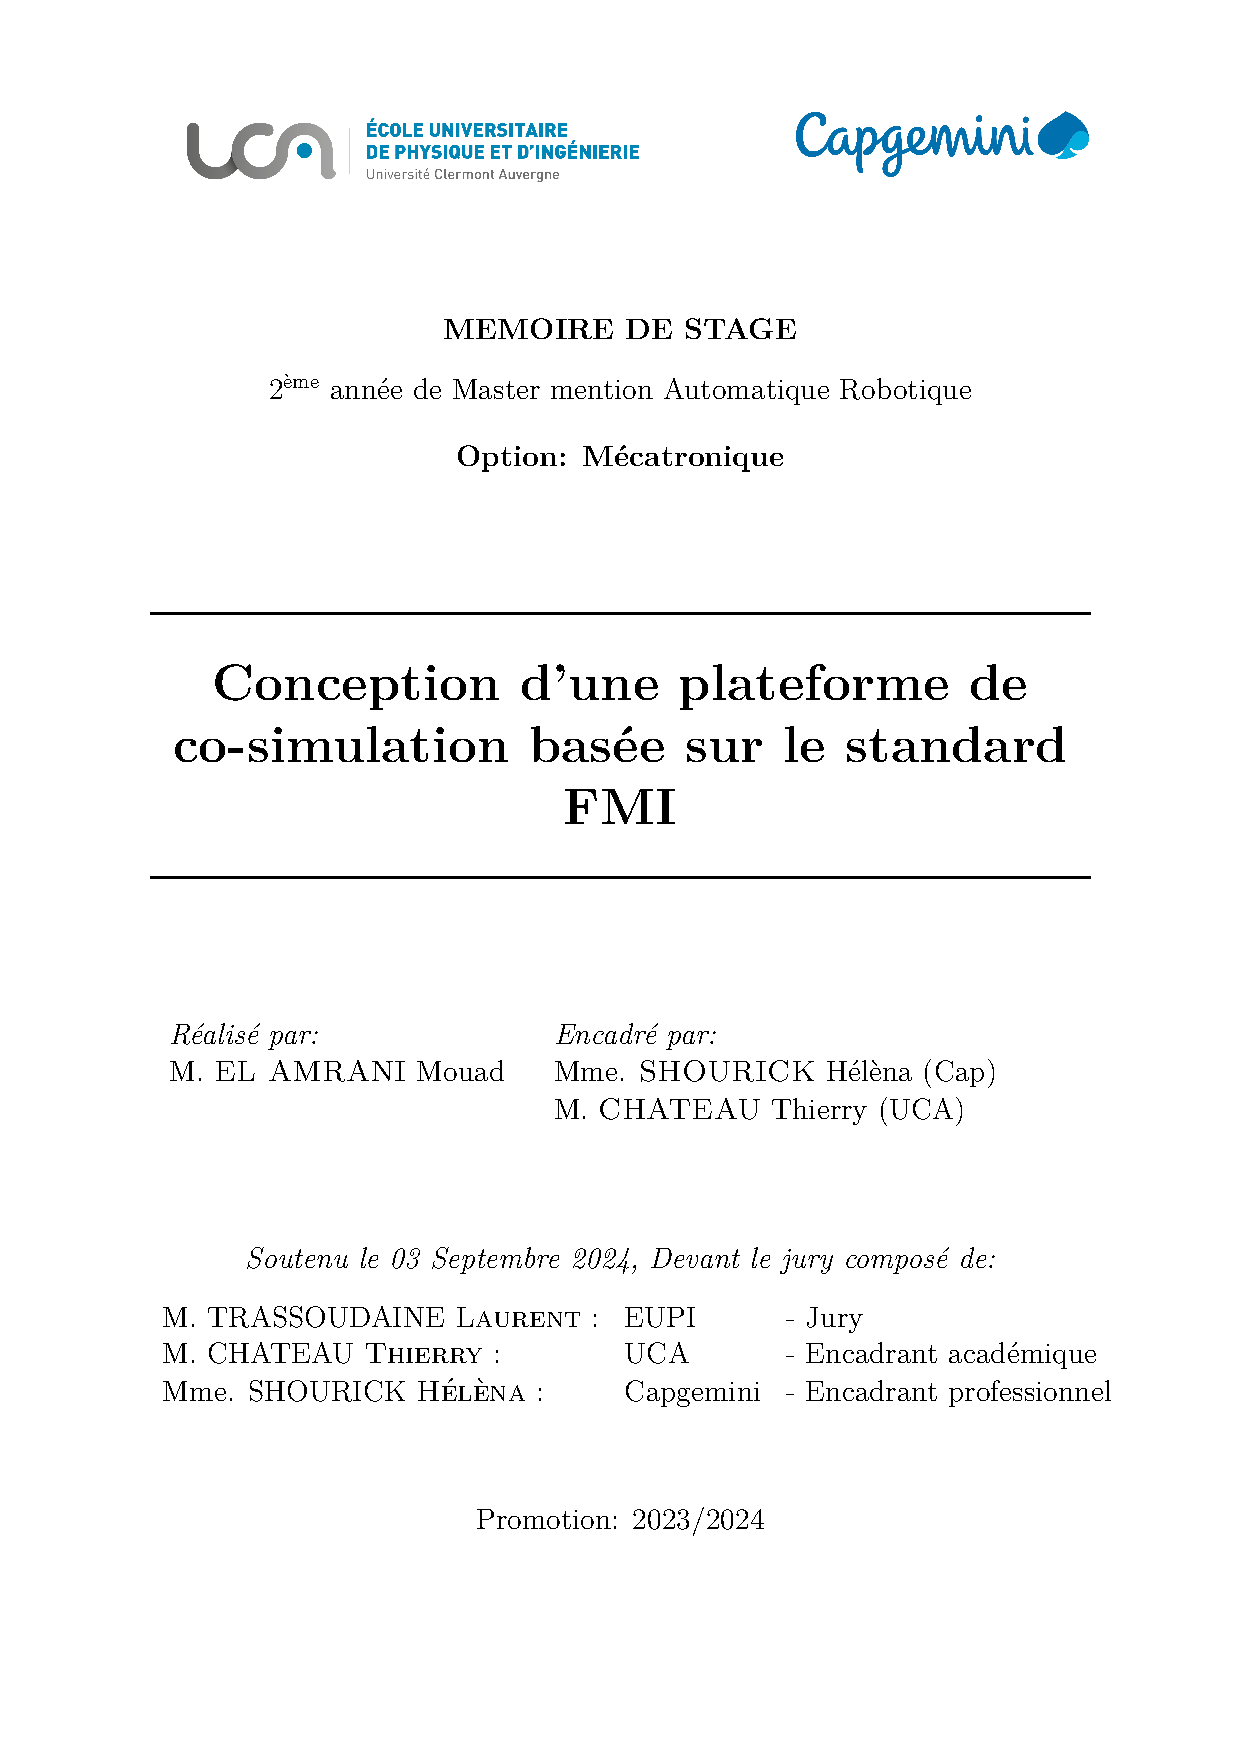
\includepdf[pages=-]{00-Page-de-garde.pdf}
\pagenumbering{Roman}
%\mychapter{0}{Dédicace}

\begin{fquote}
\begin{center}
\large{
    Je tiens à remercier chaleureusement mes \textbf{parents}, mon cher \textbf{grand-père} et \textbf{moi-même} pour cette réalisation importante. Le soutien et les conseils constants de mes parents, associés à la vision sage de mon grand-père, ont joué un rôle déterminant dans l'élaboration de mon parcours. Leur foi en mes capacités a renforcé ma détermination à réussir. Je leur suis reconnaissante de l'amour et des encouragements qu'ils m'ont prodigués tout au long de ce processus. Merci, maman, papa et grand-père, pour votre soutien inconditionnel et pour avoir été les forces motrices de ma réussite.
}
\end{center}
\bigskip
\medskip
\end{fquote}

\begin{adjustwidth}{2cm}{1cm}
\hspace*{\fill} \textbf{\textit{\large{- Mouad}}}
\end{adjustwidth}

\clearpage
%\mychapter{0}{Remerciements}

Je tiens à remercier tout d’abord mes encadrants \textbf{Mme. SHOURICK Hélèna et M. SRINIVASARENGAN Krishnan}, pour l’aide compétente qu’ils m’ont apportée, pour leur patience et leur encouragement. Leur œil critique m’a été très précieux pour structurer le travail et pour améliorer la qualité des différentes sections.

Je tiens à remercier également mon encadrant académique \textbf{M. CHATEAU Thierry} pour son temps, la qualité de son suivie ainsi que pour tous les conseils et les informations qu'il m’a prodigués.

Je tiens aussi à adresser mes plus sincères remerciements à \textbf{M. BEN AMMAR Hamza et KHASSIBA Ahmed}, chefs de projet dans l'équipe RT-SIM, pour m'offrir l'opportunité d'intégrer l'équipe et pour leur soutien.

Que les membres de jury trouvent, ici, l'expression de mes sincères remerciements pour l'honneur qu'ils me font en prenant le temps de lire et d'évaluer ce travail.

Je souhaite aussi remercier l'équipe pédagogique et administrative de l'EUPI pour leurs efforts dans le but de nos offrir une excellente formation.

Pour finir, je souhaite remercier toute personne ayant contribué de prés ou de loin à la réalisation de ce travail.


\clearpage
\mychapter{0}{Résumé}

La recherche de nouvelles approches de collaboration interdisciplinaire est essentielle pour naviguer dans les complexités du développement de systèmes face à des exigences de marché en augmentation. Une approche envisageable pour surmonter ce défi est l'adoption d'une méthode basée sur des modèles hétérogènes. Cette méthode permet à diverses équipes de créer leurs propres modèles et de conduire leurs analyses habituelles dans leur discipline respective. De plus, elle offre la possibilité de coupler ces modèles pour réaliser des simulations conjointes (co-simulation), facilitant ainsi l'analyse du comportement global du système. La norme Functional Mock-up Interface (FMI), développée par l'association Modelica, joue un rôle crucial dans la facilitation de cette intégration. FMI fournit un cadre polyvalent pour l'échange aisé de modèles et de données de simulation entre différents outils et plates-formes.
\medskip

Dans ce travail, nous présentons une approche globale de la taxonomie de la co-simulation, en utilisant des notions ontologiques pour segmenter en définissant systématiquement les divers éléments et interactions au sein des environnements de co-simulation. Cette taxonomie structurée sert de base pour améliorer la clarté et l'interopérabilité des processus de co-simulation. En outre, nous nous concentrons sur l'optimisation de l'orchestrateur d'OMSimulator, une plateforme conçue pour la co-simulation basée sur le standard FMI. Pour ce faire, nous avons employé une méthode itérative appelée méthode d'Aitken-Schwarz. En intégrant la méthode d'Aitken-Schwarz dans l'orchestrateur d'OMSimulator, nous avons pu améliorer significativement la stabilité des simulations numériques, réduire les erreurs et assurer une convergence plus rapide des résultats.
\medskip

Ces améliorations permettent de renforcer les processus de co-simulation, offrant ainsi une solution plus robuste et efficace pour le développement de systèmes complexes dans un environnement interdisciplinaire.

\medskip




\vspace{1cm}


\noindent\rule[2pt]{\textwidth}{0.5pt}

{\textbf{Mots clés :}}
Co-simulation, FMI, Taxonomie, OMSimulator, Aitken-Schwarz.
\\
\noindent\rule[2pt]{\textwidth}{0.5pt}

\clearpage

\mychapter{0}{Abstract}


The search for new approaches to interdisciplinary collaboration is essential for navigating the complexities of system development in the face of increasing market demands. One conceivable approach to overcome this challenge is the adoption of a method based on heterogeneous models. This method allows various teams to create their standard models and conduct their usual analyses within their respective disciplines. Additionally, it offers the possibility of coupling these models to perform joint simulations (co-simulation), thus facilitating the analysis of the overall system behavior. The Functional Mock-up Interface (FMI) standard, developed by the Modelica Association, plays a crucial role in facilitating this integration. FMI provides a versatile framework for the easy exchange of models and simulation data between different tools and platforms.
\medskip

In this work, we present a comprehensive approach to the taxonomy of co-simulation, using ontological notions to systematically categorize and define the various elements and interactions within co-simulation environments. This structured taxonomy serves as a basis for improving the clarity and interoperability of co-simulation processes. Furthermore, we focus on optimizing the orchestrator of OMSimulator, a platform designed for co-simulation based on the FMI standard. To achieve this, we employed an iterative method called the Aitken-Schwarz method. By integrating the Aitken-Schwarz method into the OMSimulator orchestrator, we were able to significantly improve the stability of numerical simulations, reducing errors and ensuring faster convergence of results.
\medskip

These improvements enhance the co-simulation processes, thus providing a more robust and efficient solution for the development of complex systems in an interdisciplinary environment.
\medskip

\vspace{1cm}



\noindent\rule[2pt]{\textwidth}{0.5pt}

{\textbf{Keywords :}}
Co-simulation, FMI, Taxonomy, OMSimulator, Aitken-Schwarz.
\\
\noindent\rule[2pt]{\textwidth}{0.5pt}



\clearpage
\renewcommand{\cftpartleader}{\cftdotfill{\cftdotsep}} 
\renewcommand{\cftchapleader}{\cftdotfill{\cftdotsep}} 
\newcommand{\threechecks}{\ding{51}\ding{51}\ding{51}}
\newcommand{\twochecks}{\ding{51}\ding{51}\ding{55}}
\newcommand{\onecheck}{\ding{51}\ding{55}\ding{55}}
\newcommand{\nocheck}{\ding{55}\ding{55}\ding{55}}
    \tableofcontents
\clearpage
\listoffigures
\clearpage
\listoftables

\clearpage
%\chapter*{Liste des sigles et acronymes}
\begin{acronym}[TRAD-Seg]

    \acro{ACC}{\emph{Adaptive Cruise Control}}
    \medskip
    
    \acro{ADAM}{\emph{ADAptive Moment estimation}}
    \medskip
    
    \acro{ANN}{\emph{Artificial Neural Networks}}
    \medskip
    
    \acro{CARRADA}{\emph{Camera and Automotive Radar with Range-Angle-Doppler Annotations}}
    \medskip
    
    \acro{CFAR}{\emph{Constant False Alarm Rate}}
    \medskip
    
    \acro{CNN}{\emph{Convolutional Neural Networks}}
    \medskip
    
    \acro{DFT}{\emph{Discret Fourier Transform}}
    \medskip
    
    \acro{DL}{\emph{Deep Learning}}
    \medskip
    
    \acro{DoA}{\emph{Direction of Arrival}}
    \medskip
    
    \acro{FCN}{\emph{Fully Convolutif Network}}
    \medskip
    
    \acro{FFT}{\emph{Fast Fourier transform}}
    \medskip
    
    \acro{FMCW}{\emph{Frequency Modulated Continuous Wave}}
    \medskip
    
    \acro{IoU}{\emph{Intersection over Union}}
    \medskip
    
    \acro{LiDAR}{\emph{Light Detection And Ranging}}
    \medskip
    
    \acro{MIMO}{\emph{Multi Input Multi Output}}
    \medskip
    
    \acro{ML}{\emph{Machine Learning}}
    \medskip
    
    \acro{MOT}{\emph{Multi Object Tracking}}
    \medskip
    
    \acro{Poi}{\emph{Point of interest}}
    \medskip
    
    \acro{RAD}{\emph{Range-Angle-Doppler Tensor}}
    \medskip
    
    \acro{RADAR}{\emph{Radio Detection And Ranging}}
    \medskip
    
    \acro{RADDet}{\emph{Range-Azimuth-Doppler based Radar Object Detection for Dynamic Road Users}}
    \medskip
    
    \acro{RA}{\emph{Range-Angle view}}
    \medskip
    
    \acro{RD}{\emph{Range-Doppler view}}
    \medskip
    
    \acro{SGD}{\emph{Stochastic Gradient Descent}}
    \medskip
    
    \acro{SINR}{\emph{Signal to Noise Ratio}}
    \medskip
    
    \acro{SORT}{\emph{Simple Online RealTime Tracking}}
    \medskip
    
    \acro{ToF}{\emph{Time of Flight}}
    \medskip
    
    \acro{TRAD-Seg}{\emph{Temporal RADAR Segmentation}}
    
    \end{acronym}

%%%%%%%%%%%%%%%%%%%%%%%%%%%%%%%%%%%%%%%%%%%%
%%% Content of the report and references %%%
%%%%%%%%%%%%%%%%%%%%%%%%%%%%%%%%%%%%%%%%%%%%

\cleardoublepage

\pagenumbering{arabic}
\selectlanguage{french}
\chapter*{Introduction générale}
\addcontentsline{toc}{chapter}{Introduction générale}
\markboth{Introduction générale}{Introduction générale}
\label{chap:introduction}
%\minitoc

\section*{Contexte}

Dans le domaine technologique, qui évolue rapidement, le développement de systèmes complexes exige souvent une collaboration entre plusieurs disciplines. Que ce soit en ingénierie aérospatiale, en conception automobile ou dans d'autres domaines, il est essentiel d'adopter des méthodes avancées pour naviguer à travers les complexités et interdépendances croissantes des composants de ces systèmes. Les approches traditionnelles, qui fonctionnent souvent dans des disciplines séparées, s'avèrent insuffisantes pour répondre aux exigences croissantes en matière d'efficacité, d'innovation et de performance. Il existe donc un besoin critique de nouvelles méthodologies collaboratives capables d'intégrer diverses expertises et de faciliter l'analyse complète des systèmes. L'utilisation de modèles hétérogènes et de techniques de co-simulation constitue une approche prometteuse pour relever ce défi. En permettant à différentes équipes de créer et d'analyser leurs modèles indépendamment tout en permettant des simulations intégrées, ces techniques offrent une voie vers un développement des systèmes plus robustes et plus précis. Le standard Functional Mock-up Interface (FMI), développé par l'association Modelica, apparaît comme un cadre essentiel dans le contexte de cette étude, fournissant une plateforme unifiée pour l'échange de modèles et de données entre différents outils de simulation.

\section*{Problématique}

La co-simulation, outil crucial pour analyser et développer des systèmes complexes, est souvent abordée de façon spécifique par les différents communautés scientifiques et industrielles. Cette approche fragmentée mène à un manque de standardisation et de collaboration, rendant difficile l'établissement d'une base commune et solide pour le développement du domaine. Par conséquent, les équipes interdisciplinaires rencontrent des difficultés pour adopter cette méthode, ce qui limite son utilisation et freine l'innovation dans le secteur.

En outre, la majorité des plateformes de co-simulation existantes se trouvent soit à un stade de développement alpha, soit sont insuffisamment documentées, utilisant souvent des langages propriétaires. Cette situation pose de nombreuses contraintes à l'intégration et à l'incorporation d'algorithmes d'orchestration avancés. Les utilisateurs se retrouvent face à des défis significatifs pour implémenter et optimiser ces algorithmes dans des environnements de co-simulation non standardisés, ce qui limite l'efficacité et la fiabilité des simulations numériques. Ainsi, il est impératif de développer des solutions robustes et bien documentées, basées sur des normes ouvertes comme le standard (FMI), afin de surmonter ces obstacles et de faciliter une adoption plus large et plus efficace des méthodes de co-simulation dans divers domaines.

\section*{Objectifs}
Le premier objectif de cette étude est de développer une taxonomie simplifiée et basée sur des diagrammes pour la co-simulation. En utilisant une structure ontologique claire, nous allons catégoriser et définir systématiquement les différents éléments et interactions dans les environnements de co-simulation. Les diagrammes explicatifs rendront cette approche plus accessible et intuitive pour des équipes interdisciplinaires.

Le deuxième objectif est d'étudier les différentes plateformes de co-simulation existantes. Nous analyserons les caractéristiques, avantages et limitations des principales plateformes, en mettant en lumière les défis liés à l'utilisation de langages propriétaires. Cette étude permettra d'identifier les meilleures pratiques et les lacunes actuelles.

Enfin, le troisième objectif est de mettre en place un algorithme itératif d'orchestration pour la co-simulation. Cet algorithme sera utilisé pour renforcer la stabilité des simulations numériques, minimiser les erreurs et permettre une convergence accélérée des résultats.
\section*{Organisation du mémoire}

Ce rapport est organisé en trois chapitres :

Le premier chapitre \og \textbf{\hyperref[sec:pré]{Présentation de l'organisme d'accueil et cadrage du projet}} \fg présente l'entreprise d'accueil, la méthodologie, le planning, les contraintes liées au sujet, ainsi que le cadrage du projet.

Le deuxième chapitre \og \textbf{\hyperref[sec:tax]{Taxonomie de la co-simulation}
} \fg présente une catégorisation systématique et une définition des différents éléments et interactions au sein des environnements de co-simulation en utilisant des notions ontologiques.

Le troisième chapitre \og \textbf{\hyperref[sec:orc]{Conception et développement d'un orchestrateur de co-simulation}
} \fg  explore une comparaison détaillée des différentes plateformes de co-simulation disponibles, mettant en lumière leurs caractéristiques, avantages et inconvénients. De plus, ce chapitre examine l'amélioration de l'algorithme d'orchestration, interprète les résultats obtenus et les compare avec ceux issus d'autres outils de co-simulation existants.
\medskip


\clearpage
\chapter{Présentation de l'organisme d'acceuil et cadrage du projet}
\label{sec:pré}
\section{Introduction}



\medskip

Ce chapitre présente Capgemini Engineering, une société de conseil spécialisée dans les solutions d'ingénierie, ainsi que l'équipe que j'ai intégrée et mon rôle dans le développement d'un système avancé d'aide à la conduite (ADAS) qui fonctionne efficacement dans des conditions météorologiques extrêmes.

Ce projet pose des défis uniques à cause de l'exclusivité de la technique et du nombre limité de publications disponibles sur le sujet. Cependant, il offre également des opportunités significatives de se plonger dans des domaines de pointe tels que la théorie du contrôle, l'apprentissage automatique et l'apprentissage profond. 

Ce chapitre encadre le projet et fournit un contexte permettant au lecteur de comprendre ses objectifs, sa portée et ses résultats attendus, ainsi que le rôle de Capgemini Engineering dans son développement.
\medskip
\section{Présentation de l'organisme d'accueil}
\subsection{Capgemini Engineering}
Capgemini Engineering est une filiale du groupe Capgemini qui rassemble les services
d'ingénierie et de R\&D de Capgemini Engineering, avec un chiffre d'affaires de 16 milliards
d’euros. L'expertise de Capgemini dans le domaine de production numérique ainsi que sa
connaissance sectorielle approfondie lui permettent d'accompagner les entreprises dans leur
transformation vers la 4.0 en conjuguant les mondes physique et numérique. Avec plus de 52
000 ingénieurs et scientifiques dans plus de 30 pays , Capgemini Engineering intervient dans
des secteurs variés tels que l'aéronautique, l'automobile, les sciences de la vie ou encore
l'énergie. Le groupe Capgemini, quant à lui, est un leader mondial responsable et multiculturel
comptant près de 270 000 collaborateurs dans une cinquantaine de pays. Grâce à son expertise
et son expérience, il répond à l'ensemble des besoins de ses clients, de la stratégie à la gestion
des opérations, en utilisant les dernières innovations technologiques. 
\begin{figure}[hbt!]
  \centering
  
\includegraphics[width=0.4\textwidth]{logo.png}
  \caption{Logo de la société Capgemini Engineering}
\end{figure}

En tant que partenaire stratégique, Capgemini Engineering joue un rôle essentiel dans l'accompagnement complet des projets de ses clients à travers divers secteurs industriels.
L'entreprise s'engage à fournir un niveau de service constant et de qualité, en offrant une
expertise approfondie dans chaque domaine.
Afin de répondre aux besoins spécifiques de ses clients, Capgemini Engineering adopte une
approche à la fois mondiale et locale. En tant que groupe d'envergure mondiale, il est en mesure
de proposer des solutions globales et innovantes qui répondent aux défis de l'industrie à grande
échelle. Cependant, il ne perd pas de vue l'importance d'une présence locale et d'une
compréhension approfondie des marchés spécifiques. Cela permet à Capgemini Engineering
d'offrir un accompagnement personnalisé et adapté aux exigences particulières de chaque
marché. Les clients et partenaires stratégiques de Capgemini Engineering jouent un rôle clé
dans la réussite de l'entreprise. En collaborant étroitement avec ces acteurs majeurs de
l'industrie, elle favorise l'innovation, la co-création et la recherche de solutions technologiques
avancées. Grâce à ces partenariats solides, l'entreprise est en mesure d'anticiper les tendances
du marché et de proposer des solutions différenciées qui répondent aux besoins changeants de
ses clients.
\section{Le projet RT-SIM}
L’équipe RT-SIM est composé de cinq docteurs et quatre stagiaires
(moi y compris). Le projet de recherche interne, RT-SIM, a pour but de développer
une plateforme de simulation générique, distribué et temps réel.
\subsection{Contexte}
De nos jours, le développement d’un nouveau produit dans le secteur des transports,
de l’industrie, de l’énergie et bien d’autres est devenu complexe. On souhaite
améliorer la qualité d’un produit en y intégrant de nouvelles technologies, tout en
diminuant le coût et le temps de développement.
C’est ainsi que ces dernières années, il y eut un intérêt croissant pour la simulation.
En effet, les simulateurs permettent d’intervenir sur tout le cycle en V d’un produit
et permettent ainsi d’intégrer de nouvelles technologies tout en diminuant les
coûts et le temps de développement. Les simulateurs devenant de plus en plus
réalistes, il devient de moins en moins nécessaire de développer des prototypes.
C’est ainsi qu’est né le projet RT-SIM qui souhaitait prendre en compte les nouvelles
technologies dans le développement de sa plateforme de simulation, les contraintes
imposés dans les secteurs simulés et la capacité d’être compatible dans tous les
domaines afin de pouvoir rendre un simulateur le plus réaliste possible.
\subsection{objectif}
L’objectif du projet RT-SIM est d’être :
\begin{enumerate}
  \item Générique afin de faire coexister plusieurs secteurs d’activité.
  \item Interopérable avec différents standards (ED-247 et FMI pour l’aéronautique,
  SMP2 pour le spatial, etc.), protocoles de bus de communication (CAN, ED-247,
  AFDX, etc.) et techniques de modélisation (discret et continu).
  \item Distribué avec diverses ressources informatiques connectées par Ethernet.
  \begin{figure}[hbt!]
    \centering
    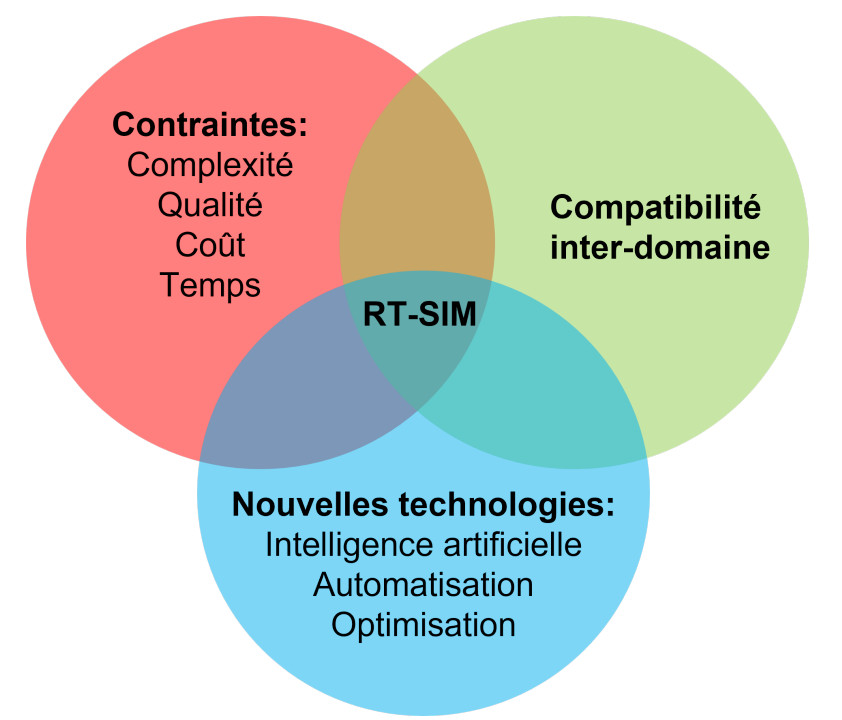
\includegraphics[width=0.5\textwidth]{2.png}
    \caption{Les motivations du projet RT-SIM}
  \end{figure}
  \item Hybride pour faire coexister ”hardware” et ”software”.
  \item Temps réel afin qu'on fassent des simulations HIL (Hardware in the loop).
\end{enumerate}
\begin{figure}[hbt!]
  \centering
  \includegraphics[width=0.5\textwidth]{3.png}
  \caption{Concept du projet RT-SIM}
\end{figure}
\section{Conclusion}

Pour conclure, dans ce chapitre nous avons présenté l’organisme d’accueil \textbf{ Capgemini Engineering} où ce projet a été réalisé, son historique, son organigramme et l’équipe de
travail. En utilisant des différents outils, nous avons mis en évidence le cadre du projet, les
objectifs visés, la démarche de travail et la planification de ce présent projet.
\\
Après, on a montré les limitations causant la problématique traitée dans ce projet, et en comparant les solutions physiques nous avons abouti à la solution physique adoptée dans ce projet.

\medskip
Dans le chapitre suivant, nous allons traiter la partie théorique de RADAR, comprendre le fonctionnement, le traitement de signal nécessaire, et la nature des données récupérées à la fin.\\
Ainsi que la motivation autour l'utilisation de l'apprentissage profond, et une définition de l'architecture des réseaux de neurones (NN).


%%% Local Variables: 
%%% m. Nous avons aussi ode: latex
%%% TeX-master: "isae-report-template"
%%% End: 
\chapter{Taxonomie de la co-simulation}\label{sec:tax}
\section*{Introduction}
Les systèmes d'ingénierie intègrent de multiples éléments dans un processus complexe, comprenant des composants physiques, des logiciels et leurs interactions. Cette complexité pose de nombreux défis pour la modélisation et pour la simulation de ces systèmes. L'une des façons de simuler des systèmes comprenant plusieurs composants consiste à modéliser et à simuler l'ensemble du système à l'aide d'un seul outil, ce que l'on appelle la simulation monolithique. L'autre approche consiste à simuler le système dans le cadre d'une co-simulation. 

La co-simulation se définit comme le couplage d'au moins deux unités de simulation distinctes. Ces unités peuvent différer par l'outil de simulation employé, l'algorithme de résolution mis en œuvre, ou encore le pas de temps de résolution utilisé. Une unité de simulation, quant à elle, représente une entité logicielle exécutable responsable de la simulation d'une partie spécifique du système \cite{1,2}. Cette approche présente un potentiel considérable et a été exploitée dans divers domaines, notamment l'industrie automobile \cite{b1}, la gestion de l'électricité \cite{b2}, le chauffage, la ventilation et la climatisation (HVAC) \cite{b3}, le domaine maritime \cite{b4}, et la robotique \cite{b5}.

Dans ce chapitre, on entreprend une révision de l'état de l'art de la co-simulation, en mettant l'accent sur le standard FMI. Notre contribution réside dans la proposition d'une nouvelle approche pour la taxonomie de la co-simulation, visant à décomposer et à simplifier l'analyse de l'état de l'art en détaillant ses fonctionnalités, les exigences et les contraintes de la co-simulation. Cette approche permet une meilleure compréhension des tenants et aboutissants de la co-simulation, ouvrant ainsi la voie à de nouvelles avancées dans ce domaine.

Dans la section \ref{sec:2}, on effectue une présentation et une critique de l'existant en introduisant le standard FMI dans le cadre de la co-simulation, la section \ref{sec:3} présente le processus d'orchestration des scénarios de co-simulation et ses contraintes. La section \ref{sec:4} contient les résultats de l'étude taxonomique menée.


\section{Le standard FMI et la co-simulation}\label{sec:2}
\subsection{FMI}
FMI (Functional Mock-up Interface) \cite{b6}, est un standard élaboré dans le but de créer une interface unifiée pour l'exécution de modèles de systèmes dynamiques, facilitant ainsi l'interopérabilité entre les outils de modélisation et de simulation. L'essence de ce standard réside dans la génération et l'échange de modèles conformes à la spécification FMI entre différents outils. Ces modèles sont, selon le standard, des FMUs (Functional Mock-up Units). 
On distingue deux modes d'utilisation principaux : l'échange de modèle (ME), où le modèle, dépourvu de solveur intégré, requiert la prise en charge de la résolution par l'utilisateur, et la co-simulation (CS), où les modèles sont exportés avec un solveur de l'outil d'import.

L'idée fondamentale derrière le FMI est de permettre aux utilisateurs de combiner des modèles provenant de divers environnements de développement et de simulation, sans être enchaînés par les restrictions d'un outil particulier. En d'autres termes, les FMUs encapsulent les modèles dans une structure standardisée, ce qui permet à ces modèles d'être facilement intégrés dans un environnement de co-simulation, où ils peuvent interagir de manière cohérente avec d'autres composants du système. Cette approche favorise la réutilisation des modèles, réduisant ainsi les efforts de développement et améliorant l'efficacité de la modélisation et de la simulation dans divers domaines d'application.

Dans le cas de la co-simulation, le standard décrit une interface discrète du modèle dynamique, par exemple, étant donnés l'état interne à l'instant $t_n$, les entrées $u_n$, le pas de communication de la co-simulation $h$, $p$ les paramètres fournis, et $y_{n+1}$ le vecteurs des sorties à l'instant $t_{n+1}= t_n + h$ peut être noté comme suit: 
\begin{equation}
    y_{n+1} = \psi_p (u_n,h)
\end{equation}

L'évolution de l'état et du temps est latente, et n'est pas décrite par le standard. Ainsi, les événements sont traités en interne. En plus, l'accès à l'état n'est possible\footnote{Pour la version 2.0.x du standard, pourtant la version 3.x offre la possibilité d'accès à tout instant t} qu'aux points de communication $n\cdot h$.

\subsection{La co-simulation }
Malgré l'intérêt grandissant pour les bénéfices et les défis scientifiques de la co-simulation, ainsi que la diversité des outils disponibles, il est à noter qu'aucune étude connue n'a encore entrepris une analyse comparative approfondie des différentes plateformes de co-simulation et de leurs limitations.

Dans l'article \cite{b7}, Gomes et al. réalisent une revue de la littérature technique portant sur les divers algorithmes développés, en segmentant la co-simulation en trois grandes catégories :
\begin{enumerate}
  \item DE : Co-simulation basée sur des événements discrets.
  \item CT : Co-simulation basée sur le temps continu.
  \item Hybride : Approche hybride de la co-simulation.
\end{enumerate}

Ils présentent ainsi une classification des algorithmes et des cas d'utilisation de la co-simulation, ce qui permet d'échanger des solutions et de fournir une compréhension plus approfondie de ce domaine. 

\section{L'orchestration de la co-simulation et ses contraintes}\label{sec:3}
\subsection{Orchestration}
La co-simulation offre la possibilité de simuler, dans un seul environnement, des systèmes conçus de manière indépendante par différents experts. Les unités de simulation, peuvent être des entités autonomes, fonctionnant potentiellement sur des machines distinctes. Pour les connecter, un orchestrateur est requis. Cet orchestrateur, également désigné sous le terme d'algorithme maître, assure le transfert des données de sortie vers les entrées, conformément à un scénario de co-simulation prédéfini, tout en supervisant la progression du temps simulé au sein de chaque unité de simulation. Les paramètres nécessaires pour garantir le bon déroulement de la co-simulation sont regroupés sous le nom de scénario de co-simulation. L'objectif principal de l'orchestrateur est de garantir que les simulations intégrées fonctionnent ensemble de manière stable et précise.

\subsection{Contraintes d'orchestration}
Dans \cite{b7}, les contraintes sont subdivisées selon la segmentation présentée. On note dans le cas d'une \textit{co-simulation basée sur des événements discrets} (DE): 
\begin{itemize}
  \item \textbf{La causalité}:  L'absence de violation de la causalité par chaque unité de simulation esclave est essentielle. Ainsi, tout orchestrateur doit veiller à maintenir cette causalité intacte lors de leur couplage.
  \item \textbf{Déterminisme et confluence}: La garantie de l'unicité de la trace de la co-simulation relève de la fonction select, comme décrit dans \cite{b7}. Une alternative à cette fonction est de s'assurer que toutes les combinaisons d'exécutions possibles conduisent toujours à la même trace de comportement, concept connu sous le nom de "confluence". Une unité de co-simulation conforme à la composition en termes de confluence l'est également en termes de déterminisme.
  \item \textbf{Structure dynamique}: Du point de vue des performances, suivre une séquence statique de dépendances peut s'avérer excessivement prudent. Avec le temps, cette chaîne de dépendances peut nécessiter des ajustements, entraînant un recours fréquent à la fonction "Rollback" pour rectifier la séquence à chaque nouvel événement, ce qui peut impacter négativement la performance de la co-simulation. Une approche dynamique de la co-simulation permet aux chaînes de dépendances d'évoluer en fonction des changements dans le comportement des unités de simulation au fil du temps.\cite{b11}
\end{itemize}

On note dans le cas d'une \textit{co-simulation basée sur le temps continu} (CT): 
\begin{itemize}
  \item \textbf{Modularité et couplage}: Simplifier le scénario de la co-simulation est une contrainte importante dans le cadre de l'orchestration. En effet, la rigidité et la protection (Boîte noire) de chaque unité de simulation impliquent des complications lors du couplage de ces derniers. (Plusieurs exemples et approches sont détaillés dans \cite{b7}). La modularité se réfère à la capacité de diviser le scénario en blocs qui peuvent être réutilisés (légèrement modifiés) dans d'autres applications.
  \item \textbf{Boucles algébriques}: On distingue globalement deux types de boucles algébriques : celles qui n'impliquent que les entrées et celles qui s'étendent sur les variables d'état. Dans \cite{b12} Kübler et Schiehlen  analysent la stabilité (zero-stability) de la co-simulation, et ils proposent deux méthodes : itérative\footnote{Une technique d'itération à point fixe qui utilise le retour en arrière (rollback) pour répéter l'étape de co-simulation avec des entrées corrigées est appelée itération dynamique, itération 'waveform relaxation' et couplage fort ou en oignon.} (résoudre les entrées inconnues pour chaque pas de simulation) ou bien éliminer les boucles algébriques en introduisant des filtres supplémentaires dans le modèle mathématique. 
  \item \textbf{Initialisation} : Par définition, la condition initiale fait partie intégrante de l'unité de simulation. Cependant, dans le contexte d'une co-simulation, la simple présence d'une condition initiale pour chaque unité ne suffit pas. Il est crucial d'établir un point de départ commun et cohérent pour l'ensemble des unités afin d'assurer une co-simulation à la fois correcte et convergente. C'est ce que l'on nomme la co-initialisation.
  \item \textbf{Contrôle d'erreur} : Évaluer la précision d'une trace de co-simulation pose un défi majeur. Idéalement, la comparaison avec la trace réelle, obtenue par la solution analytique du système continu, permettrait de quantifier l'erreur et donc la précision. Cependant, dans la pratique, l'accès à la solution analytique est souvent impossible et la connaissance du modèle complet n'est pas toujours disponible. Cette absence de référence absolue rend la mesure de la précision d'une trace de co-simulation particulièrement complexe.
\end{itemize}

La plupart des modèles ne se limitent pas exclusivement à une catégorie parmi celles mentionnées précédemment. Ils se composent souvent d'unités à la fois continues et discrètes, ce qui les classe dans la catégorie des systèmes hybrides. Cependant, il n'existe pas de standard spécifiquement défini pour ces modèles hybrides. Néanmoins, des extensions du standard FMI sont proposées dans les références \cite{b21,b22}.
\newpage 
On note que les limitations de cette approche sont : 
\begin{itemize}
  \item \textbf{Gestion du pas de communication :} En cas de gestion des événements discrets dans l'approche hybride, les événements sortants des unités de simulations peuvent être ignorés. Pour cela plusieurs approches ont été conçues telle que la gestion predictive du pas de communication \cite{b23}. 
  \item \textbf{Localisation et gestion des discontinuités :} La localisation du moment exact où un signal continu franchit un seuil est un problème bien connu, et intimement lié à l'estimation de l'avance temporelle pour prédire le pas de communication.
  \item \textbf{Stabilité et tolérance : } Il existe toujours une possibilité qu'une succession d'événements puisse causer l'instabilité du système. Des méthodes d'analyse et d'identification de ces points d'instabilités permettent d'améliorer la stabilité et rester dans les tolérances spécifiées.
\end{itemize}


\section{Taxonomie de la co-simulation}\label{sec:4}
Dans \cite{b7}, une structure arborescente est présentée, segmentant les fonctionnalités de la co-simulation, tant au niveau des plateformes que des unités. En revanche, dans l'article \cite{b24}, les auteurs proposent une taxonomie basée sur une carte mentale (Mind-Map), détaillant les options et les aspects à considérer du point de vue de l'utilisateur.

L'un des objectifs principal des taxonomies est de structurer une ontologie, de faciliter la compréhension humaine et d'aider à l’identification et la résolution des problèmes. Toutefois, la simplicité des relations taxonomiques a parfois conduit à des interprétations incomplètes, soulignant ainsi la nécessité de recourir à des techniques d'analyse plus sophistiquées. Dans ce travail, on a renforcé ces liens en utilisant des notions ontologiques \cite{b25} adaptées aux besoins spécifiques du système.

Il est également crucial de comprendre que la pensée architecturale diffère en partie de la pensée analytique classique. Raisonner en tant qu'architecte implique moins de se concentrer sur les détails opérationnels du système que sur l'identification des grands invariants structuraux. Cela permet ensuite au système de trouver son propre équilibre tout en respectant le cadre architectural qui lui a été donné, et qu'il doit préserver structurellement, comme le souligne l'article \cite{b26}.

Les propriétés qu'on utilise dans ce travail se décomposent comme suit :
\begin{itemize}
  \item Dépendances : Il existe une relation de dépendance entre deux unités lorsque l'existence et le bon fonctionnement de l'une dépendent de l'autre.
  \item Contraintes : Ces relations génèrent des conflits, que ce soit au niveau du développement ou de l'utilisation des systèmes. (Représentées par 'C')
  \item Liaisons d'hérédité : Elles se produisent lorsqu'un objet transmet un ensemble de ses propriétés à un autre. (Représentées par 'H')
  \item Approches : Ces éléments représentent les propositions destinées à l'utilisateur comme des propriétés.
  \item Objets : Ce sont des entités regroupant diverses fonctionnalités et exigences. (Représentés sous forme de tables)
\end{itemize}
\subsection{Méthodologie et résultats}
Après avoir passé en revue plusieurs articles, notamment ceux référencés \cite{b7,b8,b9,b10,b11,b12}, ainsi que les plateformes de co-simulation \cite{b13,b14,b15,b16,b17,b18,b19}, on a adopté une approche en deux étapes. Dans un premier temps, cette approche permet de mettre en évidence les exigences et les catégories fondamentales de la co-simulation. Ensuite, elle explore les contraintes, les dépendances et les différentes approches envisagées par les acteurs impliqués dans le processus de co-simulation.

Cette méthode a permis de mieux comprendre la complexité de la co-simulation en identifiant clairement les exigences et les contraintes inhérentes à cette pratique. En décomposant le processus en étapes distinctes, on a pu cerner les défis spécifiques et les besoins des utilisateurs finaux. Cette approche a également permis d'identifier les points moins traités dans la littérature.

\begin{figure}[hbt!]
  \centering
  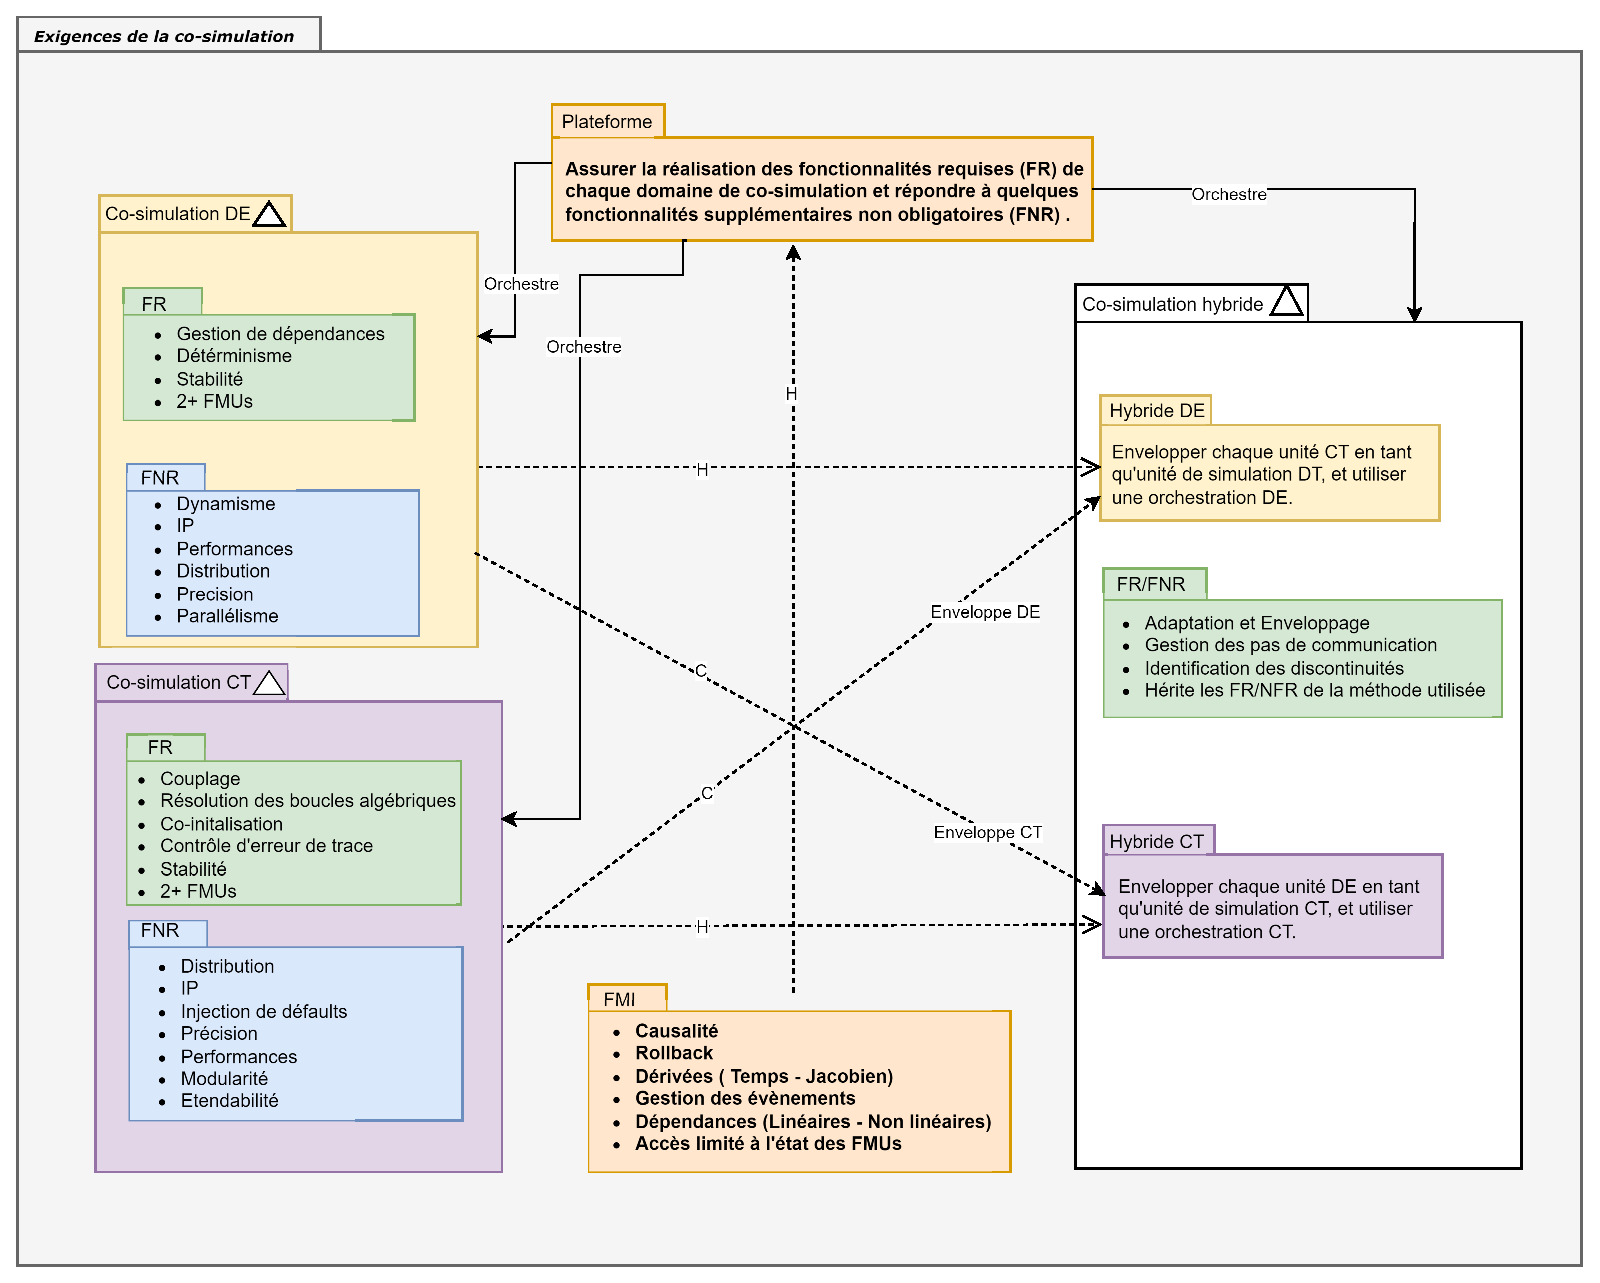
\includegraphics[width = 0.8\textwidth]{1.eps}
  \caption{Diagramme d'exigences internes de la co-simulation}
  \label{fig:1}
\end{figure}

La figure \ref{fig:1} offre une classification de la co-simulation, mettant en lumière les différentes propriétés requises ou optionnelles (FR/NFR) offertes par les divers intervenants de ce processus. Elle illustre les relations entre ces entités, telles que la liaison d'hérédité entre la plateforme et le standard FMI, offrant ainsi une vision holistique des interactions dans le domaine de la co-simulation.

D'autre part, la figure \ref{fig:2} dépeint d'une manière fonctionnelle les exigences décrites dans la figure \ref{fig:1}. En fournissant une représentation graphique du cheminement des exigences à travers les différentes entités de la co-simulation, cette figure offre une vue détaillée de la dynamique fonctionnelle de ce processus complexe.

\begin{figure}[hbt!]
  \centering
  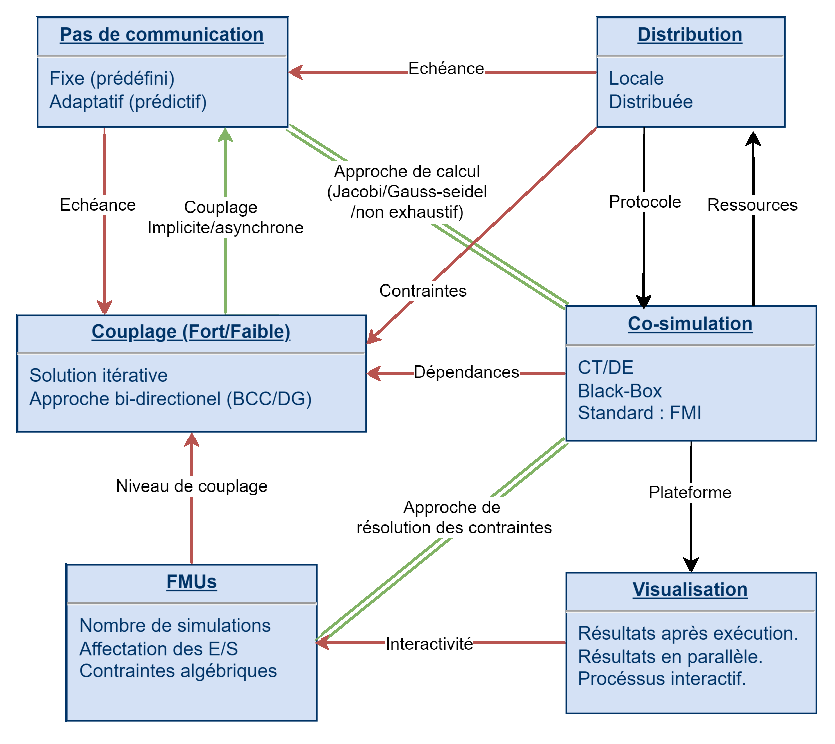
\includegraphics[width = 0.8\textwidth]{Diagramme-2.eps}
  \caption{Diagramme d'exigences fonctionnelles de la co-simulation}
  \label{fig:2}
\end{figure}


\section{Conclusion et perspectives}
Ce chapitre met en lumière les défis intrigants du domaine de la co-simulation. L'analyse commence par explorer séparément les deux principales approches : la co-simulation basée sur le temps continu et celle sur les événements discrets, avant d'examiner les difficultés associées à leur intégration. Une taxonomie basée sur des principes ontologiques et structurée en deux niveaux est ensuite introduite. La figure \ref{fig:1} illustre les interactions et les rôles des différentes entités impliquées, offrant un aperçu complet des aspects clés du processus, et servant également de modèle conceptuel pour le développement d'outils de co-simulation. Enfin, la figure \ref{fig:2} détaille les exigences de base et les approches correspondantes pour chaque entité, enrichissant ainsi notre compréhension de la structure fonctionnelle du sujet.

Au cours de cette étude, on a passé en revue plusieurs plateformes de co-simulation majeures, telles que Maestro2 \cite{b13}, OMSimulator\cite{b14} et Daccosim ng \cite{b15}. Une analyse comparative de ces plateformes, basée sur les fonctionnalités clés identifiées dans cette étude, fera l'objet du prochain chapitre.


\chapter{Plateforme de co-simulation et algorithme d'orchestration}\label{sec:orc}
\section*{Introduction}
Les plateformes de co-simulation nécessitent des algorithmes d'orchestration (OA) pour coordonner l'exécution des FMUs dans un scénario. L'OA définie comment les données sont échangées entre les FMUs dans le scénario et permet également d'influencer leur évolution d'état durant la co-simulation. Bien qu'il ne fasse pas partie de la norme FMI, l'OA est une caractéristique essentielle d'une plateforme de co-simulation. Des études ont démontré qu'il a un impact considérable sur l'exactitude des résultats de la co-simulation\cite{b7}.


Malheureusement, il n'y a pas de solution open source pour la co-simulation qui combine flexibilité, facilité d'usage et performances. Ce manque oblige ceux qui veulent personnaliser leur processus ou expérimenter avec de nouveaux algorithmes à construire leur propre système depuis le début ou reprendre un énorme travail de choix et compréhension des plateformes existantes (en prenant en compte les problèmes de licence). Ceci est particulièrement chronophage pour les grands projets, car il faut coder manuellement toutes les interactions entre les unités de simulation, prolongeant ainsi la phase préparatoire avant même de commencer à optimiser la co-simulation.

Dans ce chapitre, on va présenter une comparaison des différentes plateformes open source, où on va spécifier les points forts et faibles de chacune et argumenter le choix de notre plateforme de base (OMSimulator \cite{b14}). D'autre part, on présente le processus de développement d'un orchestrateur basé sur la méthode d'Aitken-Schwarz \cite{b27,b28}.

\section{Plateformes de co-simulation}
Le standard FMI joue un rôle essentiel dans les plateformes de co-simulation, en facilitant l'intégration et l'interopérabilité des modèles entre différents outils. Des plateformes notables comme Dymola, OpenModelica, Simulink, Maestro2 et Open Simulation Platform (OSP) utilisent largement la norme FMI pour améliorer leurs capacités de simulation. Dymola \cite{17} permet un échange de modèles et une co-simulation efficaces grâce à l'interface FMI, et prend en charge divers domaines. OpenModelica a développé OMSimulator \cite{b14}, qui peut servir comme une plateforme de co-simulation indépendante à base du standard FMI. Simulink \cite{b17}, de MATLAB, prend en charge le standard FMI à la fois en tant qu'importateur et exportateur, s'intégrant ainsi de manière transparente dans les flux de travail multi-outils. Maestro2 \cite{b13}, offre de solides fonctions de co-simulation à l'aide de FMI, visant à simplifier l'intégration de systèmes multidisciplinaires complexes. DACCOSIM NG \cite{b15}, la dernière version de la plateforme de co-simulation Daccosim, offre plusieurs fonctionnalités notamment la distribution de la co-simulation. PyFMI \cite{b16} est un package Python qui offre une interface pour travailler avec des modèles basés sur le standard FMI.
Enfin, OSP \cite{18} est une plateforme de co-simulation axée sur l'industrie maritime.

\subsection{Limites et choix}
La création d'une plateforme de co-simulation à partir de zéro est souvent inefficace et coûteuse en ressources, étant donnée la complexité de l'intégration et de la maintenance requise. Opter pour une base existante permet non seulement de réduire significativement le temps et les efforts de développement, mais aussi d'assurer une compatibilité et une robustesse initiale. La sélection d'une plateforme appropriée s'oriente selon des critères —tels que la personnalisation, les performances, SSP\footnote{Le standard SSP (System Structure and Parameterization) est conçu pour améliorer l'interopérabilité entre différents outils de simulation en permettant une description structurée des systèmes et de leurs paramètres.}, et la documentation— qui sont détaillés dans la figure \ref{fig:21}. Cette approche stratégique favorise une réalisation plus efficace des objectifs de l'étude, concentrant les efforts sur la personnalisation plutôt que sur la construction initiale.

\begin{table}[hbt!]
    \centering
    \caption{Comparaison basée sur divers critères}
    \begin{tabular}{@{}lccccc@{}} % Notice the change here to accommodate two more columns
    \toprule
    Critère & OMSimulator & Maestro2 & OSP & pyFMI & Daccosim NG \\ % Added pyFMI and Daccosim NG
    \midrule
    Personnalisation & \twochecks & \threechecks & \onecheck & \twochecks & \onecheck \\ % Example data
    Performances & \threechecks & \threechecks & \onecheck & \twochecks & \twochecks \\ % Example data
    Documentation & \threechecks & \onecheck & \nocheck & \twochecks & \onecheck \\ % Example data
    Facilité d'utilisation & \threechecks & \onecheck & \twochecks & \threechecks & \twochecks \\ % Example data
    Support de SSP  & \threechecks & \twochecks & \twochecks & \twochecks & \onecheck \\ % Example data
    Modularité & \twochecks & \threechecks & \onecheck & \nocheck & \twochecks \\ % Example data
    Distribution & \nocheck & \nocheck & \nocheck & \twochecks & \threechecks \\ % Example data
    Langage  & C++ & Java & C++ & Python & C++ \\ % Adjusted to include programming languages
    \bottomrule
    \end{tabular}
    \label{fig:21}
\end{table}

J'ai opté pour OMSimulator pour plusieurs raisons convaincantes. Tout d'abord, il bénéficie d'une documentation riche et accessible, ce qui facilite grandement l'apprentissage et l'utilisation de l'outil. Sa structure et sa conception soignées garantissent également une expérience utilisateur fluide et aisée. De plus, OMSimulator est un outil déjà bien développé, offrant une base solide pour tout projet de co-simulation. Un autre point fort est l'activité continue de son équipe de développement sur GitHub, ce qui témoigne de leur engagement à améliorer constamment l'outil et à soutenir sa communauté d'utilisateurs. Cette combinaison de facteurs fait d'OMSimulator le choix idéal pour ce projet.

\subsection{OMSimulator}

OMSimulator \cite{b14} est développé en tant que bibliothèque de simulation autonome en open source, dotée d'une interface utilisateur complète en C. Son intégration dans l'éditeur graphique OpenModelica OMEdit illustre l'utilisation de l'interface C-API pour créer une expérience utilisateur graphique et intuitive. En outre, OMSimulator propose une interface en ligne de commande (CLI), des interfaces de script pour Python et Lua, permettant son intégration dans divers outils tiers et applications spécialisées, tels que des simulateurs de vol.

Dans OMS, les modèles composites sont structurés sous forme d'un arbre hiérarchique composé de blocs de construction spécifiques. Le nœud racine de cet arbre peut être un système TLM, un système faiblement couplé (système WC) ou un système fortement couplé (système SC), chacun se distinguant par la manière dont les connexions sont gérées : 
\begin{itemize}
    \item Les systèmes \textbf{TLM} contiennent des connexions TLM, qui peuvent être considérées comme des connexions retardées motivées par la physique.
    \item Les systèmes faiblement couplés \textbf{Weakly-Coupled} sont utilisés pour la co-simulation. Toutes les unités de simulation fonctionnent de manière indépendante et sont synchronisées par un algorithme maître à certains moments de la communication.
    \item Les systèmes fortement couplés \textbf{Strongly-Coupled} sont utilisés pour regrouper les FMUs-ME dans une unité de co-simulation. Ils partagent un solveur commun et utilisent un schéma de communication continu. 
\end{itemize}
On a étudié la documentation générée à travers Doxygen\footnote{\url{https://www.doxygen.nl/}} et le source code fournit\footnote{\url{https://github.com/OpenModelica/OMSimulator}} afin de créer une documentation plus ciblée qui servira de guide pour les futures modifications par l'équipe RTSIM. Cette documentation spécifique est présentée dans l'annexe \ref{app:documentation}.  Il est important de noter que notre étude se concentre particulièrement sur l'approche des systèmes faiblement couplés (WC) et que tous les FMUs utilisés pour les démonstrations dans cette recherche sont des FMUs-CS.

\subsection{Interface d'utilisation OMS}

Dans notre contexte, on se sert de la version lignes des commandes, ainsi que l'interface python pour la rédaction des scénarios de co-simulation. 

Dans la configuration d'OMSimulatorPython, le fichier `capi.py` joue un rôle essentiel puisqu'il utilise `ctypes`, une bibliothèque Python pour appeler des fonctions C depuis Python. Cela permet aux scripts Python d'accéder directement et d'utiliser les fonctionnalités de simulation sous-jacentes fournies par OMSimulator. En utilisant `ctypes` pour établir des liaisons avec des fonctions C, `capi.py` convertit efficacement ces fonctions en fonctions que l'on peut invoquer en Python. Autour de ce fichier central, d'autres modules Python tels que `Model.py`, `System.py`, et `Scope.py` s'appuient sur ces liaisons pour offrir une API plus abstraite, permettant aux utilisateurs de gérer les  scénarios de co-simulation plus facilement. Cette architecture non seulement simplifie l'intégration de tâches de simulation complexes dans les scripts Python, mais maintient également les avantages de performance de l'implémentation C native, comblant ainsi le fossé entre la facilité de scriptage de haut niveau et la puissance computationnelle de bas niveau.

Dans la figure \ref{tab:A2}, on présente un script Python pour lancer une co-simulation d'un amplificateur différentiel divisé en deux FMUs comme présenté dans la figure suivante :

\begin{figure}[hbt!]
    \centering
    \begin{minipage}[b]{0.45\textwidth}
        \includegraphics[width=\textwidth]{leftfmu.png}
    \end{minipage}
    \begin{minipage}[b]{0.45\textwidth}
      \includegraphics[width=\textwidth]{rightfmu.png}
  \end{minipage}
  \caption{Modèles des FMUs utilisés dans la co-simulation de l'amplificateur différentiel}
  \label{fig:21}
  \end{figure}

  \section{Génération des FMUs}
  Transformer un modèle ou un ensemble d'équations en un FMU , qui compile essentiellement ces éléments en un ensemble de code C et de bibliothèques, présente un ensemble unique de défis et d'opportunités. Cette transformation implique l'encapsulation du comportement dynamique du modèle dans une unité compilée autonome qui interagit avec divers environnements de simulation via le standard FMI. Cependant, la compilation multi-plateforme représente un problème notable. Assurer le fonctionnement sans faille d'un FMU sur différents systèmes d'exploitation (Windows, Linux, MacOS) peut être complexe en raison des différences entre les compilateurs, les bibliothèques et les architectures systèmes.
  
  On présente quelques outils de génération des FMUs testés dans cette étude : 
  \begin{itemize}
    \item \textbf{SIMULINK} :  On utilise le Simulink Coder en combinaison avec le FMI Kit pour générer des FMUs à partir des modèles Simulink. Cette méthode permet d'exporter les modèles sous forme de FMUs, supportant la co-simulation ou l'échange de modèles. Le processus inclut la configuration du modèle Simulink pour l'exportation, la sélection des réglages appropriés du solveur, puis l'utilisation de la fonction d'exportation du FMI Kit pour finaliser l'exportation.
    \item \textbf{OpenModelica} : OpenModelica offre un support intégré pour l'exportation de modèles sous forme de FMUs. On charge simplement le modèle dans OpenModelica et on utilise la commande exportToFMU(). Cette commande permet de spécifier différentes options, telles que la compatibilité de version (FMI 1.0 ou 2.0), et le choix entre l'exportation pour la co-simulation ou l'échange de modèles. On peut également utiliser le drapeau supplémentaire "-d=fmuExperimental". Ce drapeau permet d'activer des fonctionnalités expérimentales spécifiques qui ne sont pas encore standard dans la version stable de OpenModelica tel que : fmi2GetSpecificDerivatives, canGetSetFMUState, canSerializeFMUstate.
    \item \textbf{Source Code FMU (pythonfmu)} : Ces dernières années, plusieurs cadres logiciels open-source ont été développés pour l'exportation des FMUs à partir du code source. CPPFMU, développé par SINTEF Ocean dans le cadre du projet ViProMa, propose une interface C++ de haut niveau avec des fonctionnalités telles que les exceptions et la gestion automatique de la mémoire pour écrire du code maîtres/esclaves conforme à FMI. Cependant, il ne prend pas en charge la génération du fichier 'modelDescription.xml' ni le conditionnement des FMUs. FMUSDK, fourni par QTronic, est un SDK basé sur C permettant l'utilisation des FMUs pour l'échange de modèles et la co-simulation, et qui supporte jusqu'à la version 2.0 de FMI, mais il manque également la génération automatique du modelDescription.xml. JavaFMI, développé par l'institut SIANI et financé par l'EIFER, et FMI4j, développé en Kotlin et sous licence MIT, prennent tous deux en charge l'importation et l'exportation de FMUs sur la JVM, FMI4j utilise CPPFMU pour la mise en œuvre des fonctions FMI et se concentre sur la performance grâce à l'intégration JNI. JavaFMI emploie une approche plus impérative utilisant le passage de messages, tandis que FMI4j utilise un style déclaratif avec des annotations, conduisant à des différences dans la performance et l'interaction utilisateur dans la définition du modèle.
    \begin{table}[hbt!]
        \centering
        \begin{tabular}{|c|c|c|c|}
          \hline
          \textbf{Tool} & \textbf{Target language} & \textbf{Target platform} & \textbf{FMI version} \\ \hline
          JavaFMI & JVM & Win, Linux & 2.0 \\ \hline
          FMI4j & JVM & Win, Linux & 2.0 \\ \hline
          CPPFMU & C++ & Win, Linux  & 1.0 \& 2.0 \\ \hline
          FMUSDK & C & Win, Linux, OSX  & 1.0 \& 2.0 \\ \hline
          Pythonfmu & python & Win, Linux & 1.0 \& 2.0 \\
          \hline
        \end{tabular}
        \caption{Comparaison des différents outils d'export des FMUs}
      \end{table}

      PythonFMU \footnote{\url{https://github.com/NTNU-IHB/PythonFMU}} \cite{26} est une plateforme logicielle sous licence MIT qui facilite l'empaquetage de code Python "3.x" en FMUs de co-simulation. Développé en collaboration entre NTNU et Safran Tech, il est accessible via pip ou conda. Bien qu'il fonctionne immédiatement sur les systèmes Windows et Linux 64 bits, PythonFMU requiert une distribution Python compatible déjà installée sur le système cible, ainsi que toute bibliothèque tierce nécessaire. On présente dans \ref{tab:A3}, notre script python pour créer un FMU correspondant à une source de courant.
    \item \textbf{uniFmu} \footnote{\url{https://github.com/INTO-CPS-Association/unifmu/tree/}} \cite{27}: Universal Functional Mock-up Unit est un outil qui permet l'implémentation des FMUs dans n'importe quel langage de programmation. Ce framework fournit des binaires pré-compilés pour Windows, Linux et macOS, évitant ainsi les complications liées à la cross-compilation et à la configuration de chaînes d'outils complexes. Il intègre également un mécanisme d'extension facile à utiliser, permettant la prise en charge de divers langages de programmation. De plus, une interface en ligne de commande est disponible pour générer rapidement des FMUs à l'aide d'une seule commande.
  \end{itemize}

  \section{Orchestration de la co-simulation}
  L'algorithme orchestrateur est chargé de gérer l'échange de données et la synchronisation entre ses composants, assurant ainsi que la simulation globale respecte les contraintes temporelles et les exigences de précision préétablies. Il prend en charge des tâches telles que la gestion des pas de temps, le contrôle des erreurs et la séquence d'exécution des différentes unités de simulation. En orchestrant la manière et le moment où ces FMUs échangent des données, l'algorithme maître vise à assurer que les simulations restent cohérentes et pertinentes.
\subsection{Orchestrateurs d'OMS}

Comme mentionné dans \ref{sec:WC}, on s'intéresse à la classe SystemWC.cpp. On présente dans cette section les deux algorithmes orchestrateurs d'OMS.
\begin{table}[h]
    \centering
    \begin{adjustbox}{width=\textwidth}
    
    \begin{tabular}{|c|c|c|}
    \hline
    \textbf{Solveur} & \textbf{Type} & \textbf{Description} \\ \hline
    oms\_solver\_wc\_ma & wc-system & Algorithme maître par défaut à pas fixe \\ \hline
    oms\_solver\_wc\_mav & wc-system & Algorithme maître à pas adaptatif \\ \hline
    oms\_solver\_wc\_mav2 & wc-system & Algorithme maître à pas adaptatif (double pas) \\
    \hline
    \end{tabular}
\end{adjustbox}
    \caption{Description des orchestrateurs utilisés dans les systèmes wc}
    \end{table}

    On note d'abord des points en commun entre ces différents orchestrateurs: 
    \begin{itemize}
        \item Méthode \textbf{stepUntil} : Responsable de l'avancement du temps des différents FMUs présents dans le scénario. 
        \item Méthode \textbf{getInputAndOutput} : Cette méthode traite les connexions entre les composants au sein d'un graphe dirigé pour extraire et gérer les valeurs d'entrée et de sortie pour les FMUs capables de gérer leur propre état. Elle parcourt les connexions triées, en excluant les boucles algébriques, et remplit les vecteurs avec les valeurs des signaux réels des composants FMU connectés.
        \item Méthode \textbf{SolveAlgLoop} : Cette méthode offre à l'utilisateur le choix entre deux solveurs pour résoudre les boucles algébriques, en fonction de la complexité du problème. KINSOL de SUNDIALS est idéal pour les systèmes d'équations non linéaires complexes grâce à ses méthodes robustes comme celles de Newton, adaptées aux modèles de grande envergure nécessitant des calculs précis de Jacobien. En revanche, FixedPointIteration (Algorithme de Tarjan) est plus adapté pour les systèmes moins complexes, utilisant une itération de point fixe qui permet une résolution rapide et efficace pour des problèmes d'ingénierie standard.
    \end{itemize}

Dans \ref{tab:A4}, on décrit l'algorithme qui illustre le fonctionnement de l'algorithme maître utilisant une taille de pas adaptative. Le principe repose sur la gestion de l'erreur, définie comme la différence entre les interfaces de deux états successifs, où le système est régulé en fonction de la magnitude de l'erreur. Cette dernière est indicative du dynamisme du système. On note trois points faibles de cet algorithme : 
\begin{itemize}
    \item \textbf{Contrôle de la Taille de Pas} : Si les tailles de pas maximum et minimum sont mal ajustées, cela pourrait empêcher la convergence de l'algorithme ou causer de l'instabilité par des pas trop grands.
    \item \textbf{Gestion des Erreurs} : La méthode calcule l'erreur et utilise un facteur de sécurité pour décider des rollbacks. Une mauvaise calibration de ces seuils peut entraîner des rollbacks inutiles ou insuffisants, affectant l'efficacité et la précision de la simulation.
    \item \textbf{Stabilité numérique et convergence}: L'algorithme ajuste dynamiquement les tailles de pas en fonction de la réponse du système, ce qui présente un risque d'instabilité numérique si les ajustements de pas ne sont pas en accord avec les propriétés numériques du système. Cela pourrait entraîner des solutions qui ne convergent pas ou un comportement divergent, particulièrement dans les systèmes sensibles ou très dynamiques.
\end{itemize}

Dans \ref{tab:A6}, on décrit l'algorithme utilisé par oms\_solver\_wc\_ma, qui implémente une méthode de pas fixe pour la simulation. Cet algorithme intègre également la sauvegarde des états des composants pour permettre des rollbacks en cas d'erreurs durant les étapes de simulation. Deux aspects critiques de cet algorithme sont notés :
\begin{itemize}
    \item \textbf{Adaptabilité aux Modèles Non Linéaires et Complexes}: Les simulations qui impliquent des modèles non linéaires ou ayant des comportements complexes posent des défis particuliers pour les méthodes à pas fixe. 
    \item \textbf{Critères de Convergence}: Pour garantir que l'algorithme aboutisse à une solution correcte et stable, il est important d'établir des critères de convergence bien définis et bien personnalisé. Dans le cas d'une méthode à pas fixe, où le seul degré de liberté réside dans la modification des dérivées des signaux d'entrée, cette approche peut s'avérer limitée face à la dynamique de certains systèmes.
\end{itemize}
Cela met en lumière l'importance d'adopter une méthode qui marie l'adaptabilité du pas de communication, l'optimisation des critères de convergence, et une gestion d'erreur solide, tout en maintenant la complexité des calculs à un niveau minimal.

\section{Orchestrateur Aitken-Schwarz}

Dans les sections précédentes, nous avons abordé plusieurs problèmes et défis liés à la co-simulation, incluant l'instabilité causée par le pas de communication et les mécanismes d'estimation et de contrôle d'erreurs. Ces difficultés sont largement reconnues et étudiées dans la littérature scientifique. Dans \cite{29}, une méthode itérative est proposée, qui assure la cohérence des interfaces tout en éliminant les discontinuités à chaque macro-étape. Cette méthode a été comparée à d'autres approches bien établies, telles que la co-simulation non itérative type Jacobi, la co-simulation itérative avec conservation de l'ordre zéro \cite{b12}, et un algorithme non itératif amélioré pour le lissage des variables \cite{30}. 

Dans notre travail, nous considérons un algorithme de couplage en point fixe basé sur la technique de décomposition du domaine de Schwarz dans lequel nous avons utilisé un Schwarz additif (ASM) \cite{b27}. Ces méthodes itératives peuvent être convergentes ou divergentes en fonction du partitionnement du domaine et des conditions aux limites. En outre, nous avons utilisé la propriété de convergence ou de divergence purement linéaire (c'est-à-dire que l'opérateur d'erreur de la méthode ne dépend pas du nombre d'itérations) pour accélérer la méthode itérative vers la vraie solution avec la technique d'accélération de la convergence d'Aitken, même avec une méthode divergente \cite{b28}.

Il est important de noter que, dans notre contexte, l'accélération est spécifiquement appliquée à la résolution de l'interface. De plus, ces méthodes sont non intrusives pour les FMUs, ce qui les rend particulièrement adaptées à la co-simulation de systèmes de type boîte noire (FMU-CS).



\subsection{Implémentation de la méthode Aitken-Schwarz}

On note $z(t_n)$ le vecteur contenant les différents variables de l’interface du modèle au pas de communication $t_n$, où $z(t_n) \in \mathbb{R}^N$. Le vecteur $z(t_{n+1})$ l'interface après un pas de communication (c'est-à-dire après un appel de la fonction \textbf{stepUntil} $\mathcal{S}$).
\begin{equation}
    z(t_{n+1}) = \mathcal{S} (z(t_n))
\end{equation}

Le principe de cette méthode consiste à réaliser, au cours d'un unique pas de communication, plusieurs itérations (c'est-à-dire de multiples pas de simulation sans progression temporelle), jusqu'à ce que le critère de convergence soit atteint ou qu'une limite maximale d'itérations soit dépassée.

\begin{equation}
    Z^{k+1}= \mathcal{S} (Z^{k})
\end{equation}
où k est l'indice d'itérations de Schwarz. En outre, comme montré dans \cite{b28}: 
\begin{equation}
    Z^{k+1}-Z^0 = \mathbb{P} (Z^k-Z^0)
\end{equation}
on peut extraire de l'équation (2.3) la forme généralisé de l’accélération d'aitken:
\begin{equation}
    Z^{\infty} = (Id_N - \mathbb{P} )^{-1} (Z^{1}-\mathbb{P} Z^0)
\end{equation}
En définissant l'erreur entre les valeurs à l'interface pour les itérations (k+1) et (k) de la manière suivante : $e^k = (Z^{k+1}-Z^k)$, il est possible de calculer algébriquement l'opérateur $\mathbb{P}\in\mathbb{R}^{N\cdot N}$ à partir de l'équation (2.3) après $N+1$ itérations. Cette démarche est réalisable si la matrice $[e^N,\dots, e^1]$ est inversible, et s'effectue de la manière suivante : 
\begin{equation}
    \mathbb{P} = [e^{N+1},\dots, e^2]\cdot[e^N,\cdots, e^1]^{-1}
\end{equation}
Cet opérateur d'erreur doit uniquement être calculé lors de la première étape. Toutefois, si la topologie évolue ou en présence de non-linéarités, il sera nécessaire de recalculer l'opérateur.\cite{b28}

La méthode a été implémenté dabs un méta-modèle de co-simulation et testé avec un circuit RL. Le code correspondant est présenté dans \ref{tab:A7}.
\subsection{Implémentation dans OMSimulator}

L'algorithme qui décrit l'intégration de la méthode Aitken-Schwarz dans OMS est présenté dans la figure ci-dessous :
\begin{figure}[hbt!]
    \label{fig:AS} 
    \centering
    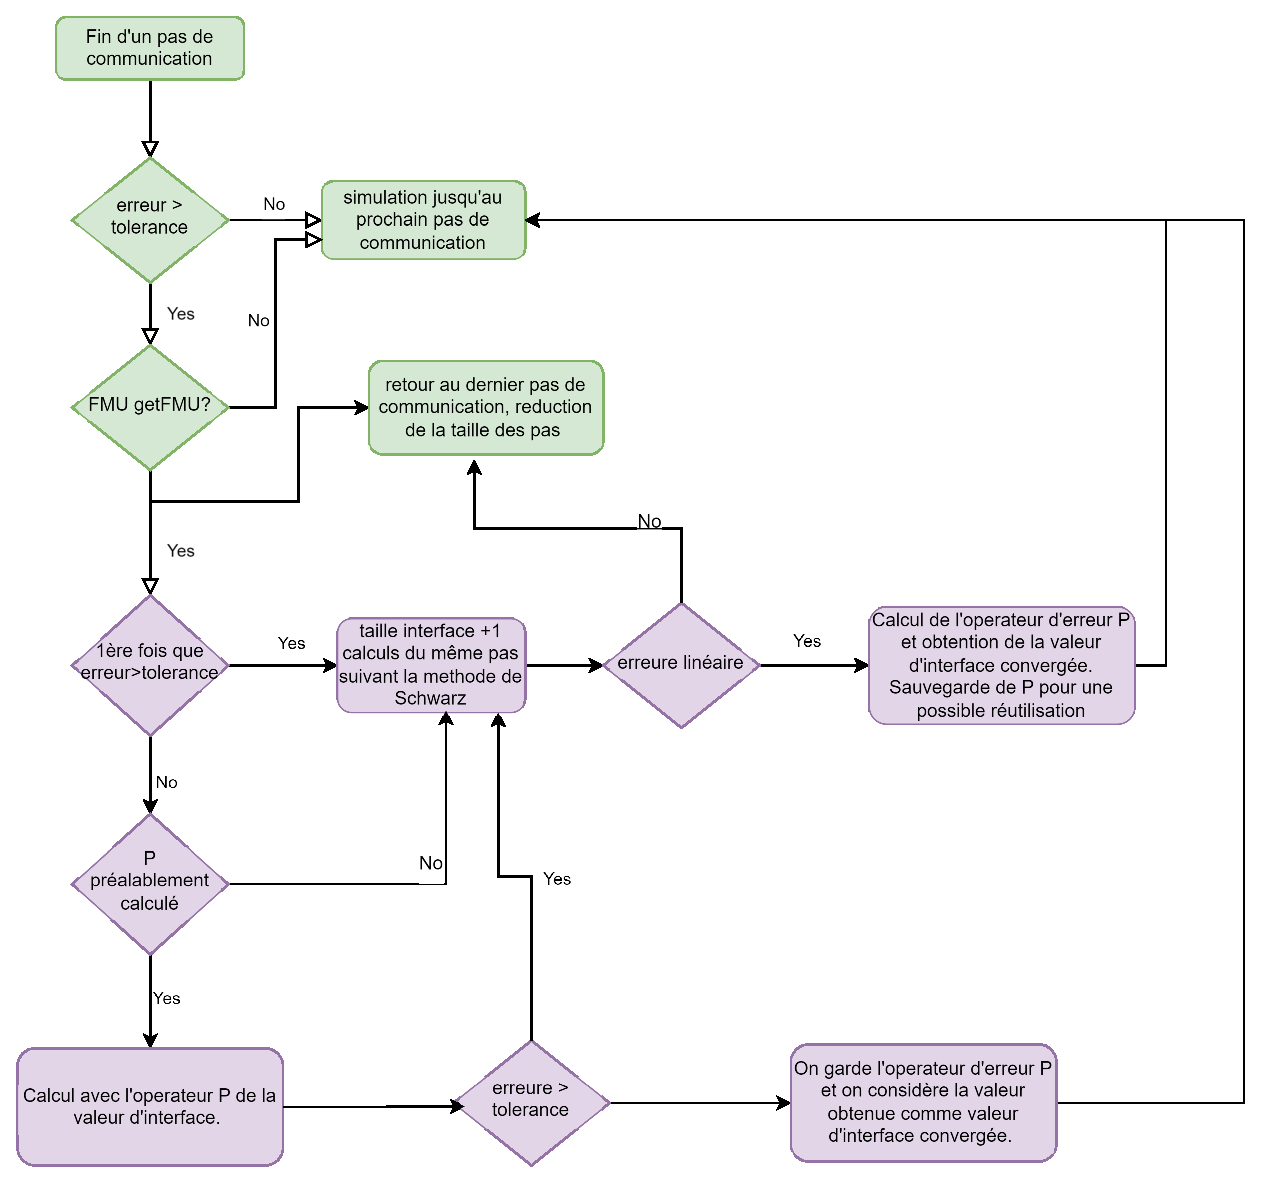
\includegraphics[width = 0.9\textwidth]{ajoutAitkenOPS.drawio.eps}
    \caption{Intégration de la méthode Aitken-Schwarz dans l'orchestrateur}
\end{figure}

L'algorithme repose sur le principe du rollback et requiert donc des FMUs compatibles avec cette fonctionnalité.
\subsection{Tests et résultats}

Pour générer des scénarios de co-simulation, on a découpé des modèles OpenModelica, avant de les exporter sous forme de FMUs. On effectue dans cette section, des tests et comparaison entre trois algorithmes orchestrateurs : 
-  oms\_solver\_wc\_ma (Rollback et modification de dérivée) - oms\_solver\_wc\_AS (Rollback et Aitken-Schwarz) - Orchestrateur simple avec tolérance relative.
 
\begin{figure}[hbt!]
    \centering
    \begin{minipage}[b]{0.45\textwidth}
        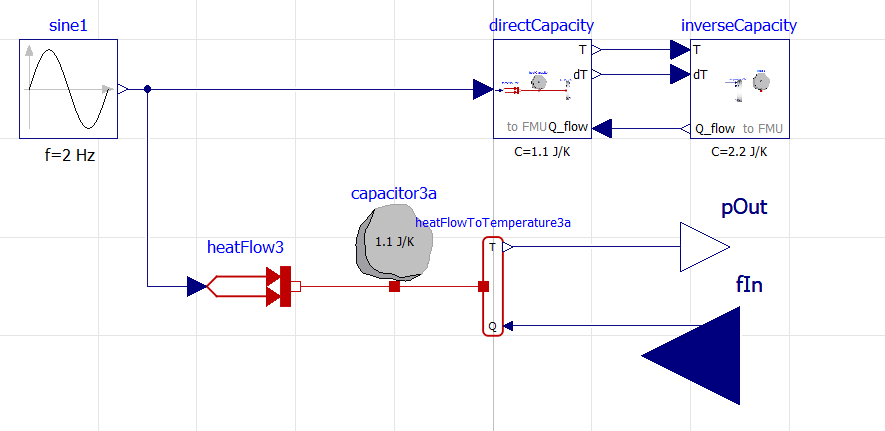
\includegraphics[width=\textwidth]{GenerationfmuL.png}
    \end{minipage}
    \begin{minipage}[b]{0.45\textwidth}
      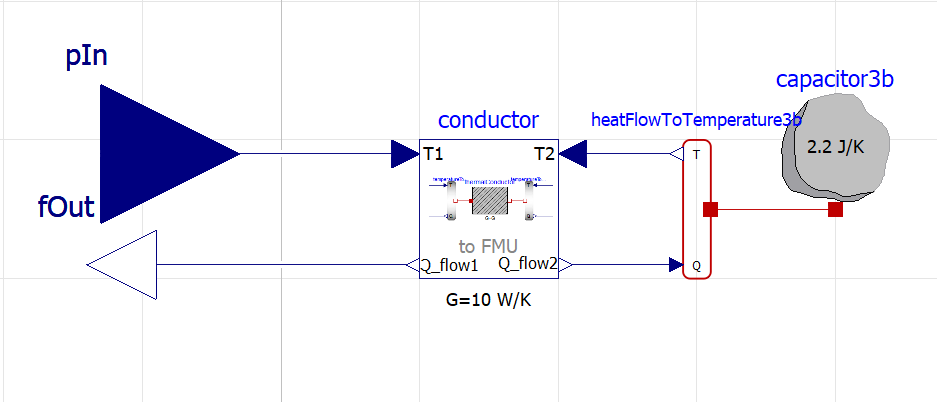
\includegraphics[width=\textwidth]{GenerationfmuR.png}
  \end{minipage}
  \caption{Modèles des FMUs utilisés dans la co-simulation de l'amplificateur différentiel}
  \label{fig:23}
  \end{figure}
Ce modèle est utilisé pour effectuer une co-simulation d'un système thermique avec une entrée sinusoïdale influençant des propriétés thermiques telles que la capacité et la conductance. On a découpé le modèle pour créer un point d'échange (pOut (Température T) et fIn (Flux de chaleur Q)). On présente dans la figure \ref{fig:24} une comparaison entre la simulation monolithique du modèle et sa co-simulation avec l'orchestrateur à pas fixe 'ma' d'OMS.

\begin{figure}[hbt!]
    \centering
    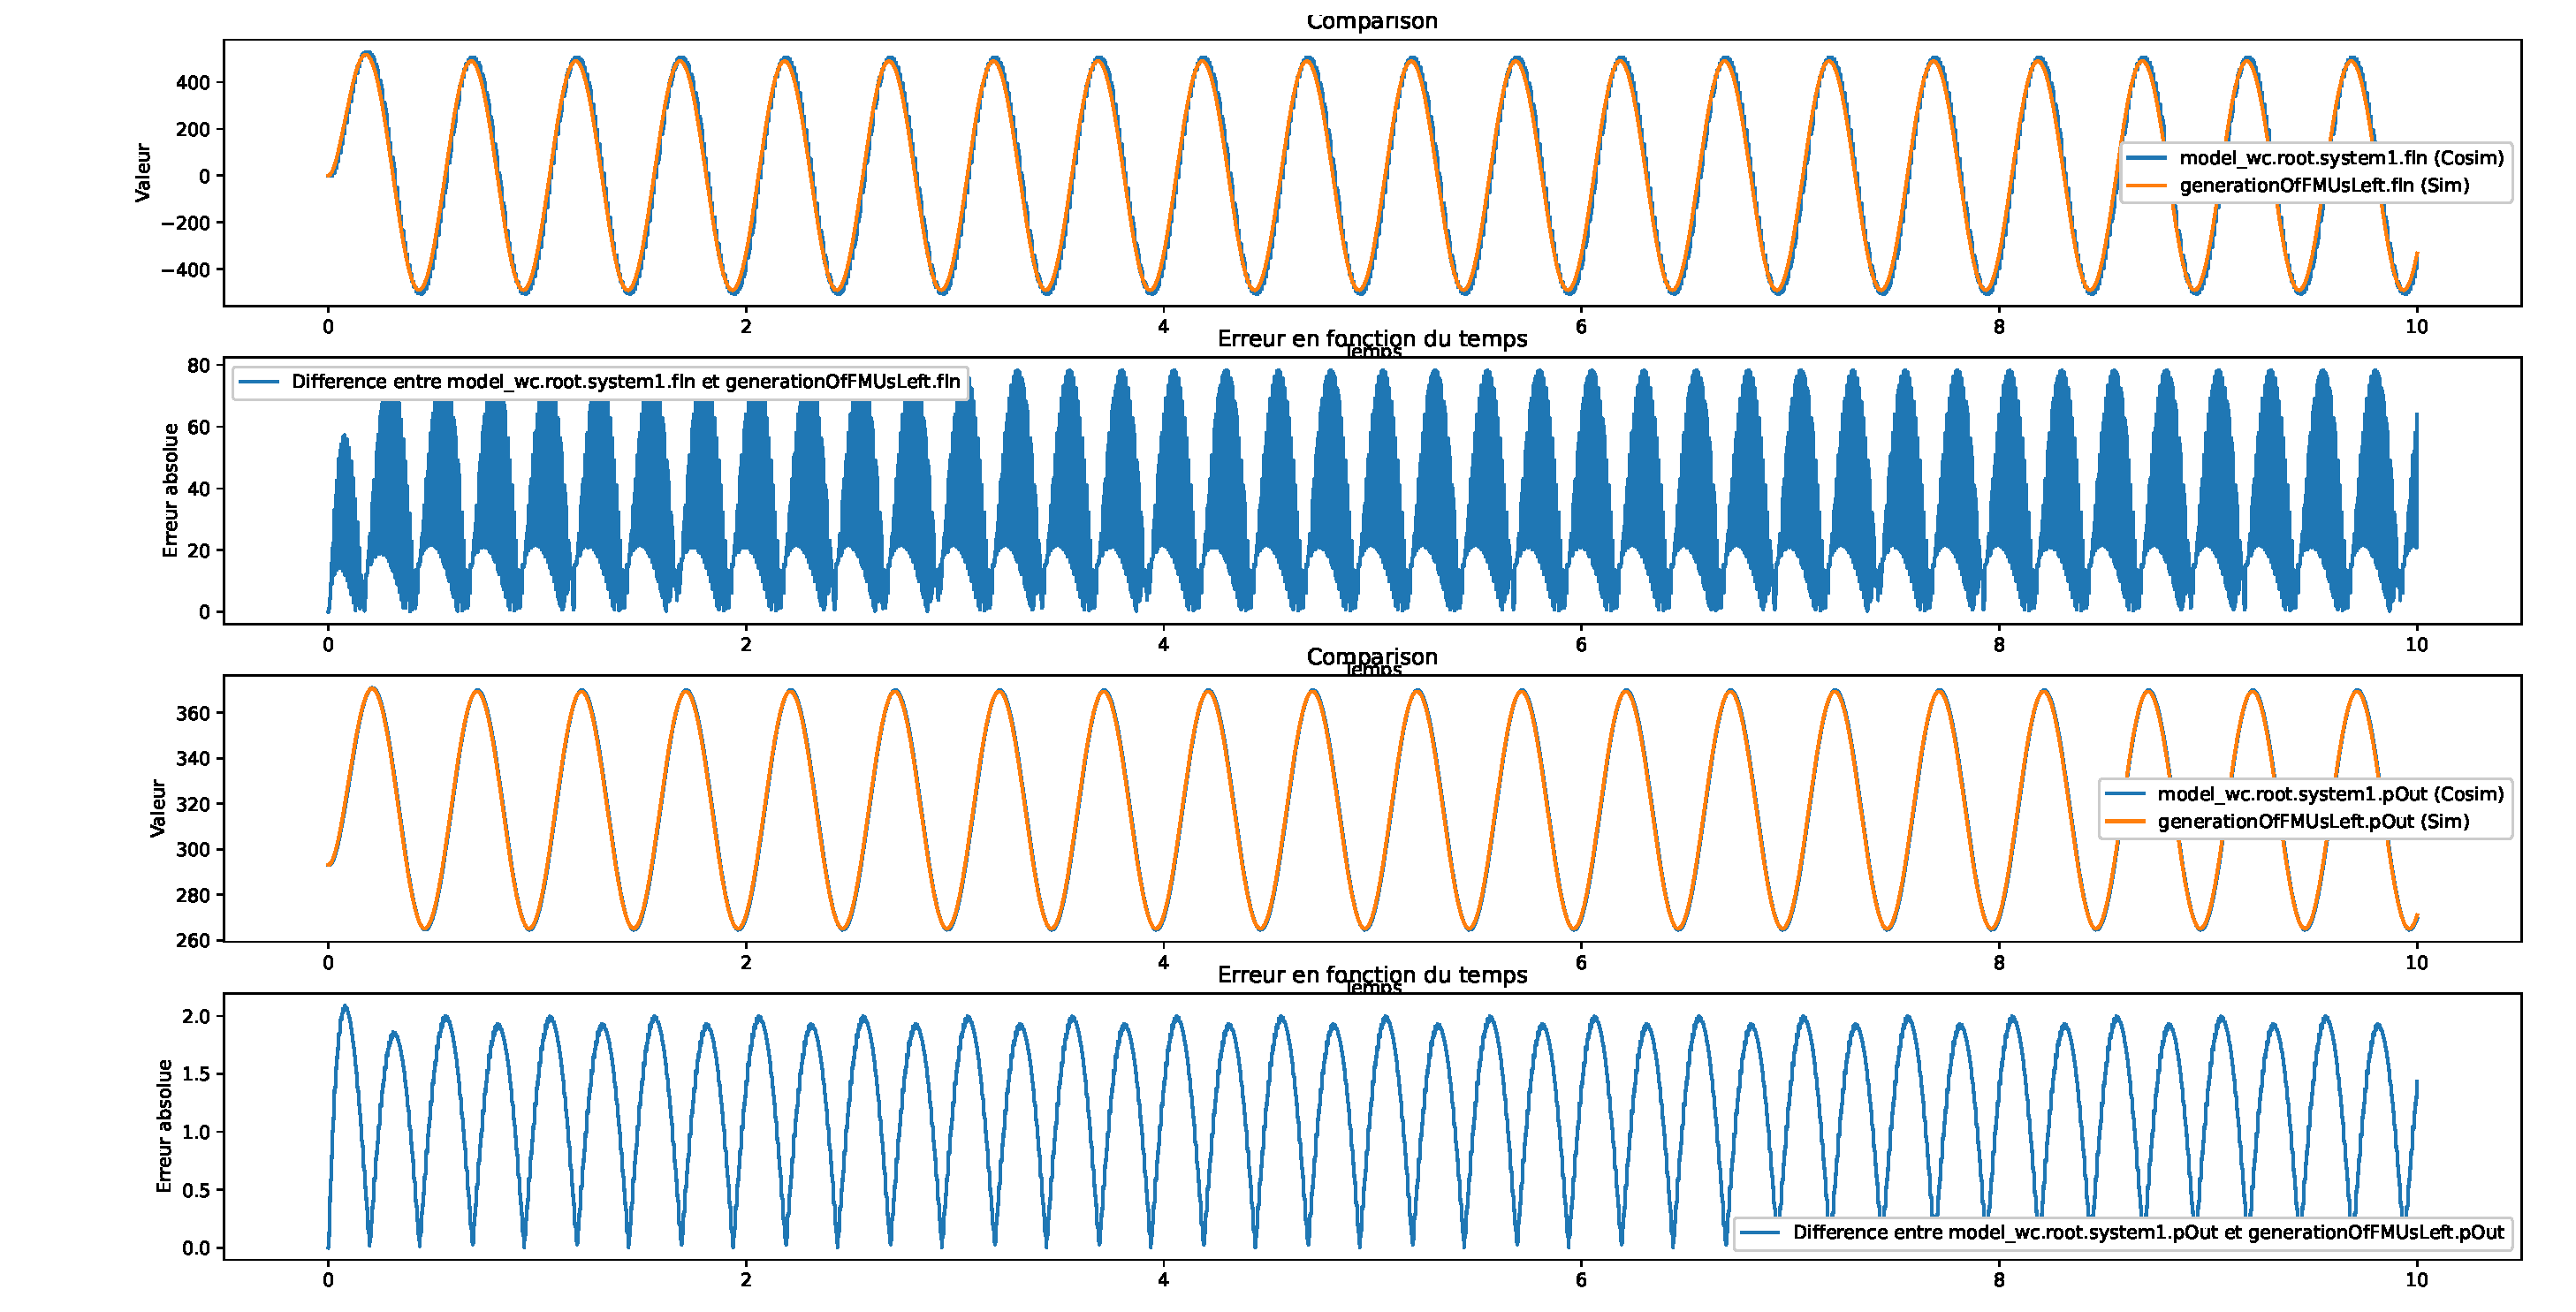
\includegraphics[width =\textwidth]{generationFMUOMS.eps}
    \caption{Comparaison de l'orchestrateur d'OMS avec une simulation monolithique du modèle \ref{fig:23}}
    \label{fig:24}
\end{figure}

Dans la figure \ref{fig:25}, nous présentons une comparaison similaire en utilisant notre orchestrateur Aitken-Schwarz. Les deux figures incluent également l'erreur absolue entre l'algorithme souhaité et la simulation monolithique du modèle. Les paramètres préfixés par "generationOffFMUs" proviennent de la simulation monolithique, tandis que ceux commençant par "model\_wc.root.systemX" sont issus de la co-simulation.
\newpage
\begin{figure}[hbt!]
    \centering
    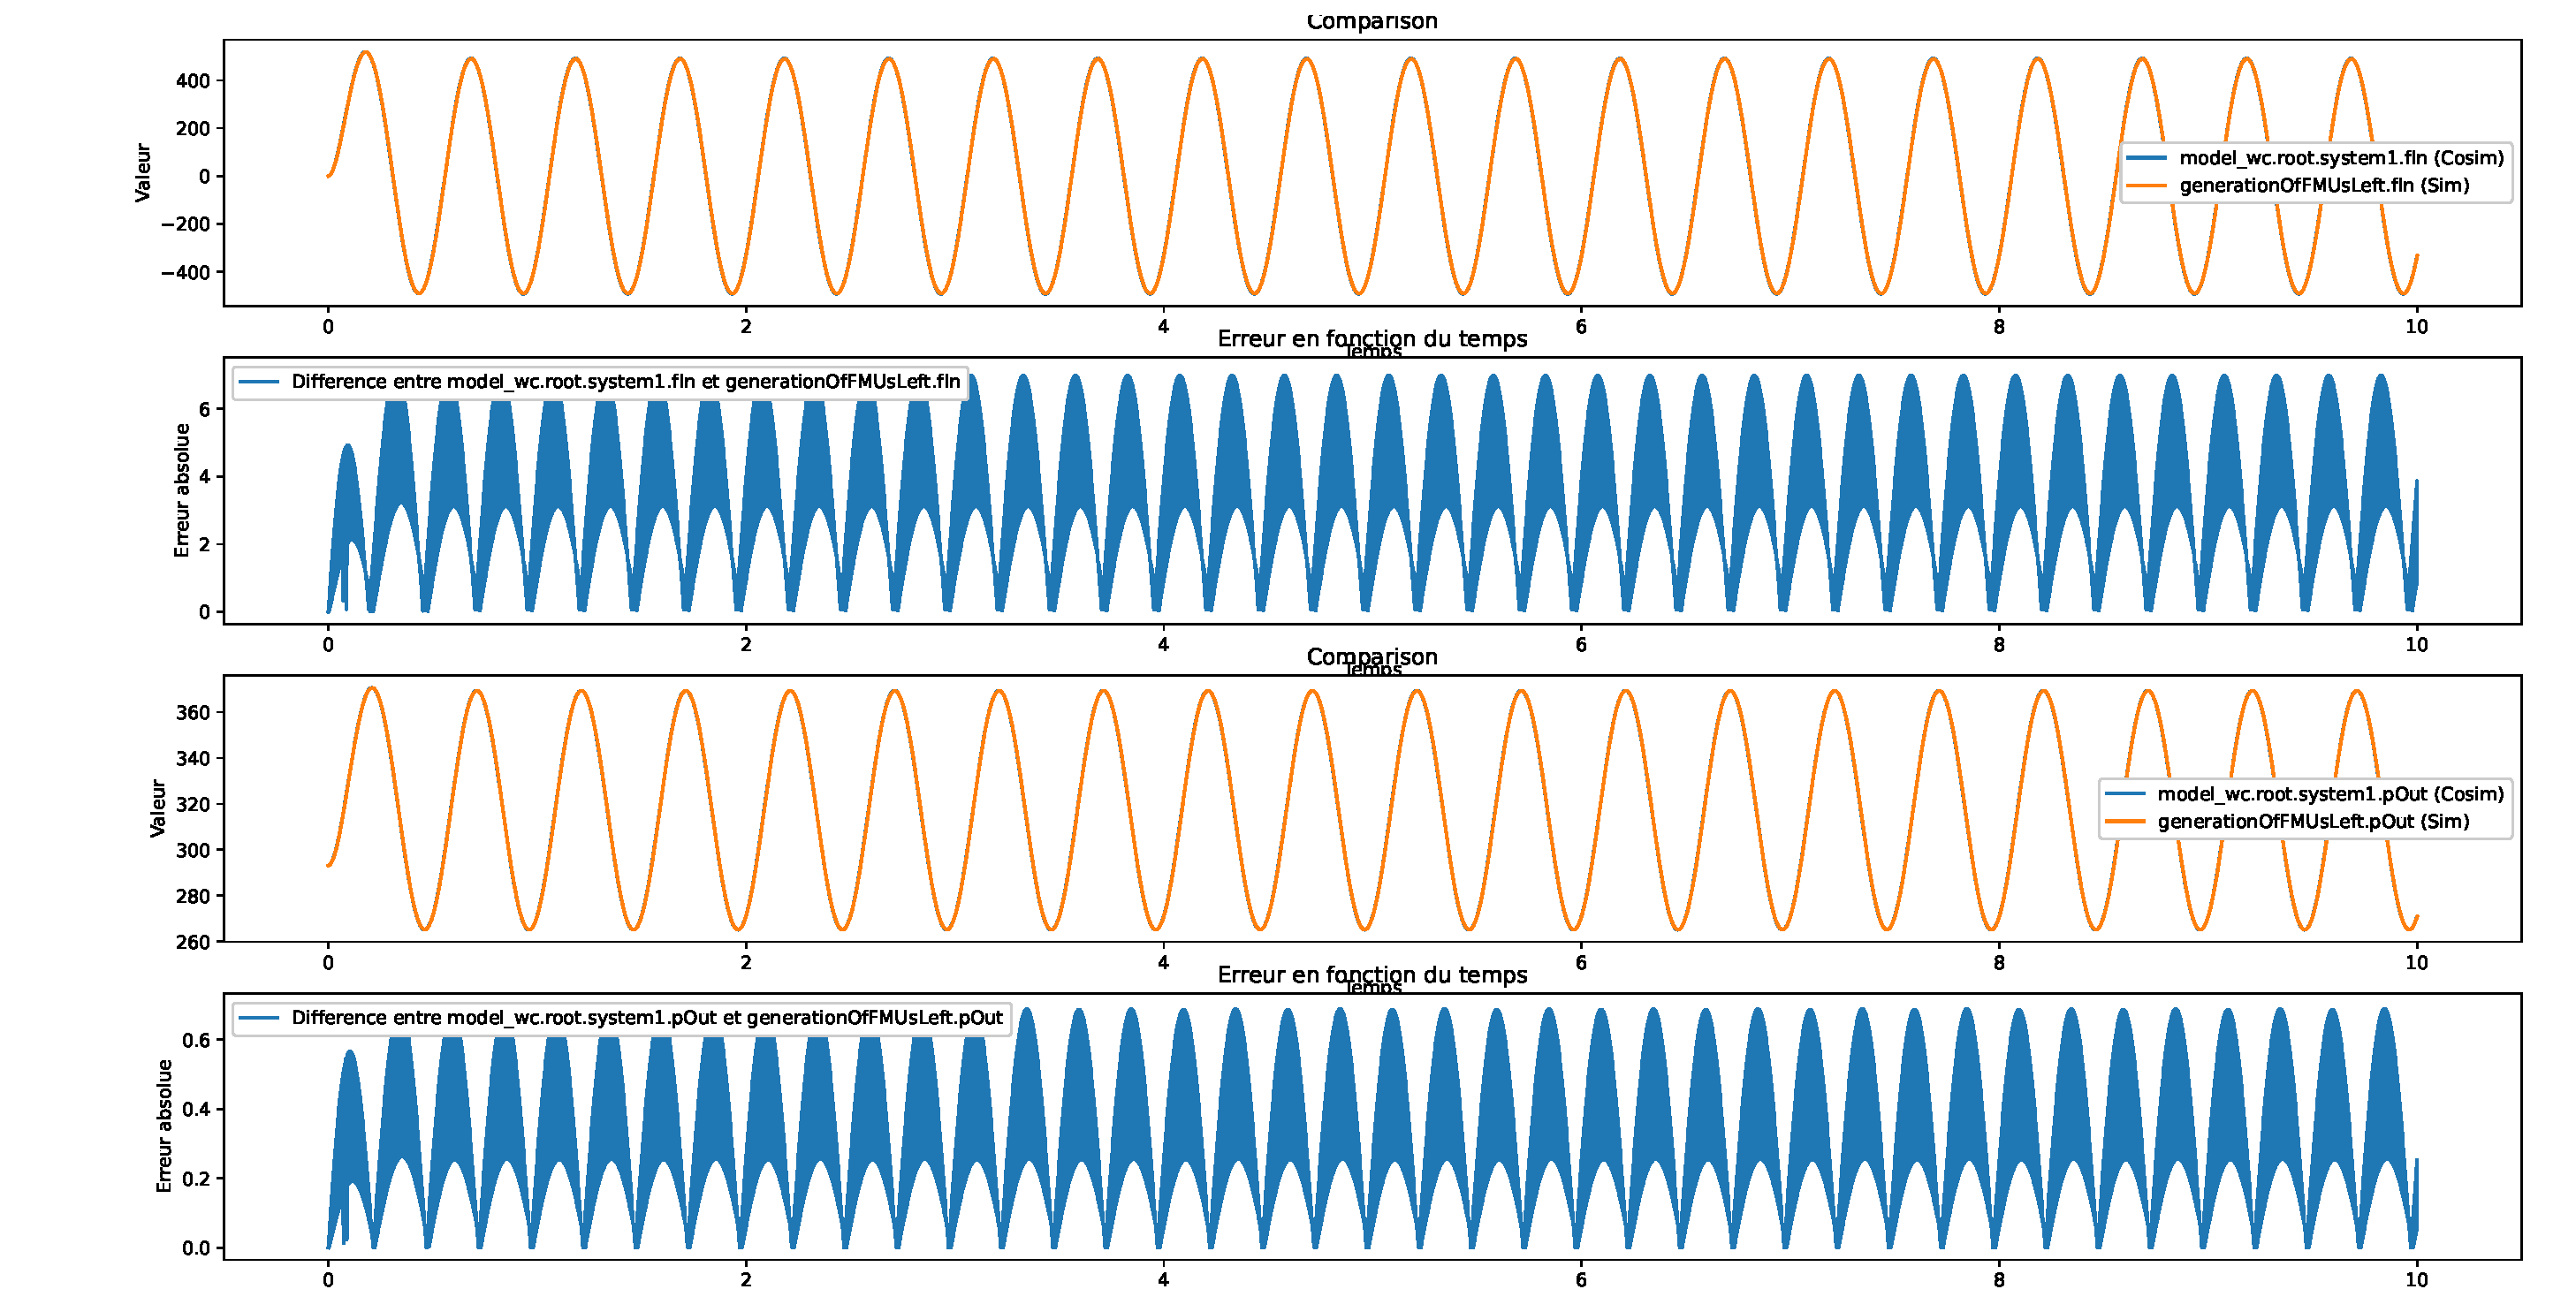
\includegraphics[width =\textwidth]{generationFMUSchwarz.eps}
    \caption{Comparaison de l'orchestrateur Aitken-Schwarz avec une simulation monolithique du modèle \ref{fig:23}}
    \label{fig:25}
\end{figure}
\begin{figure}[hbt!]
    \centering
    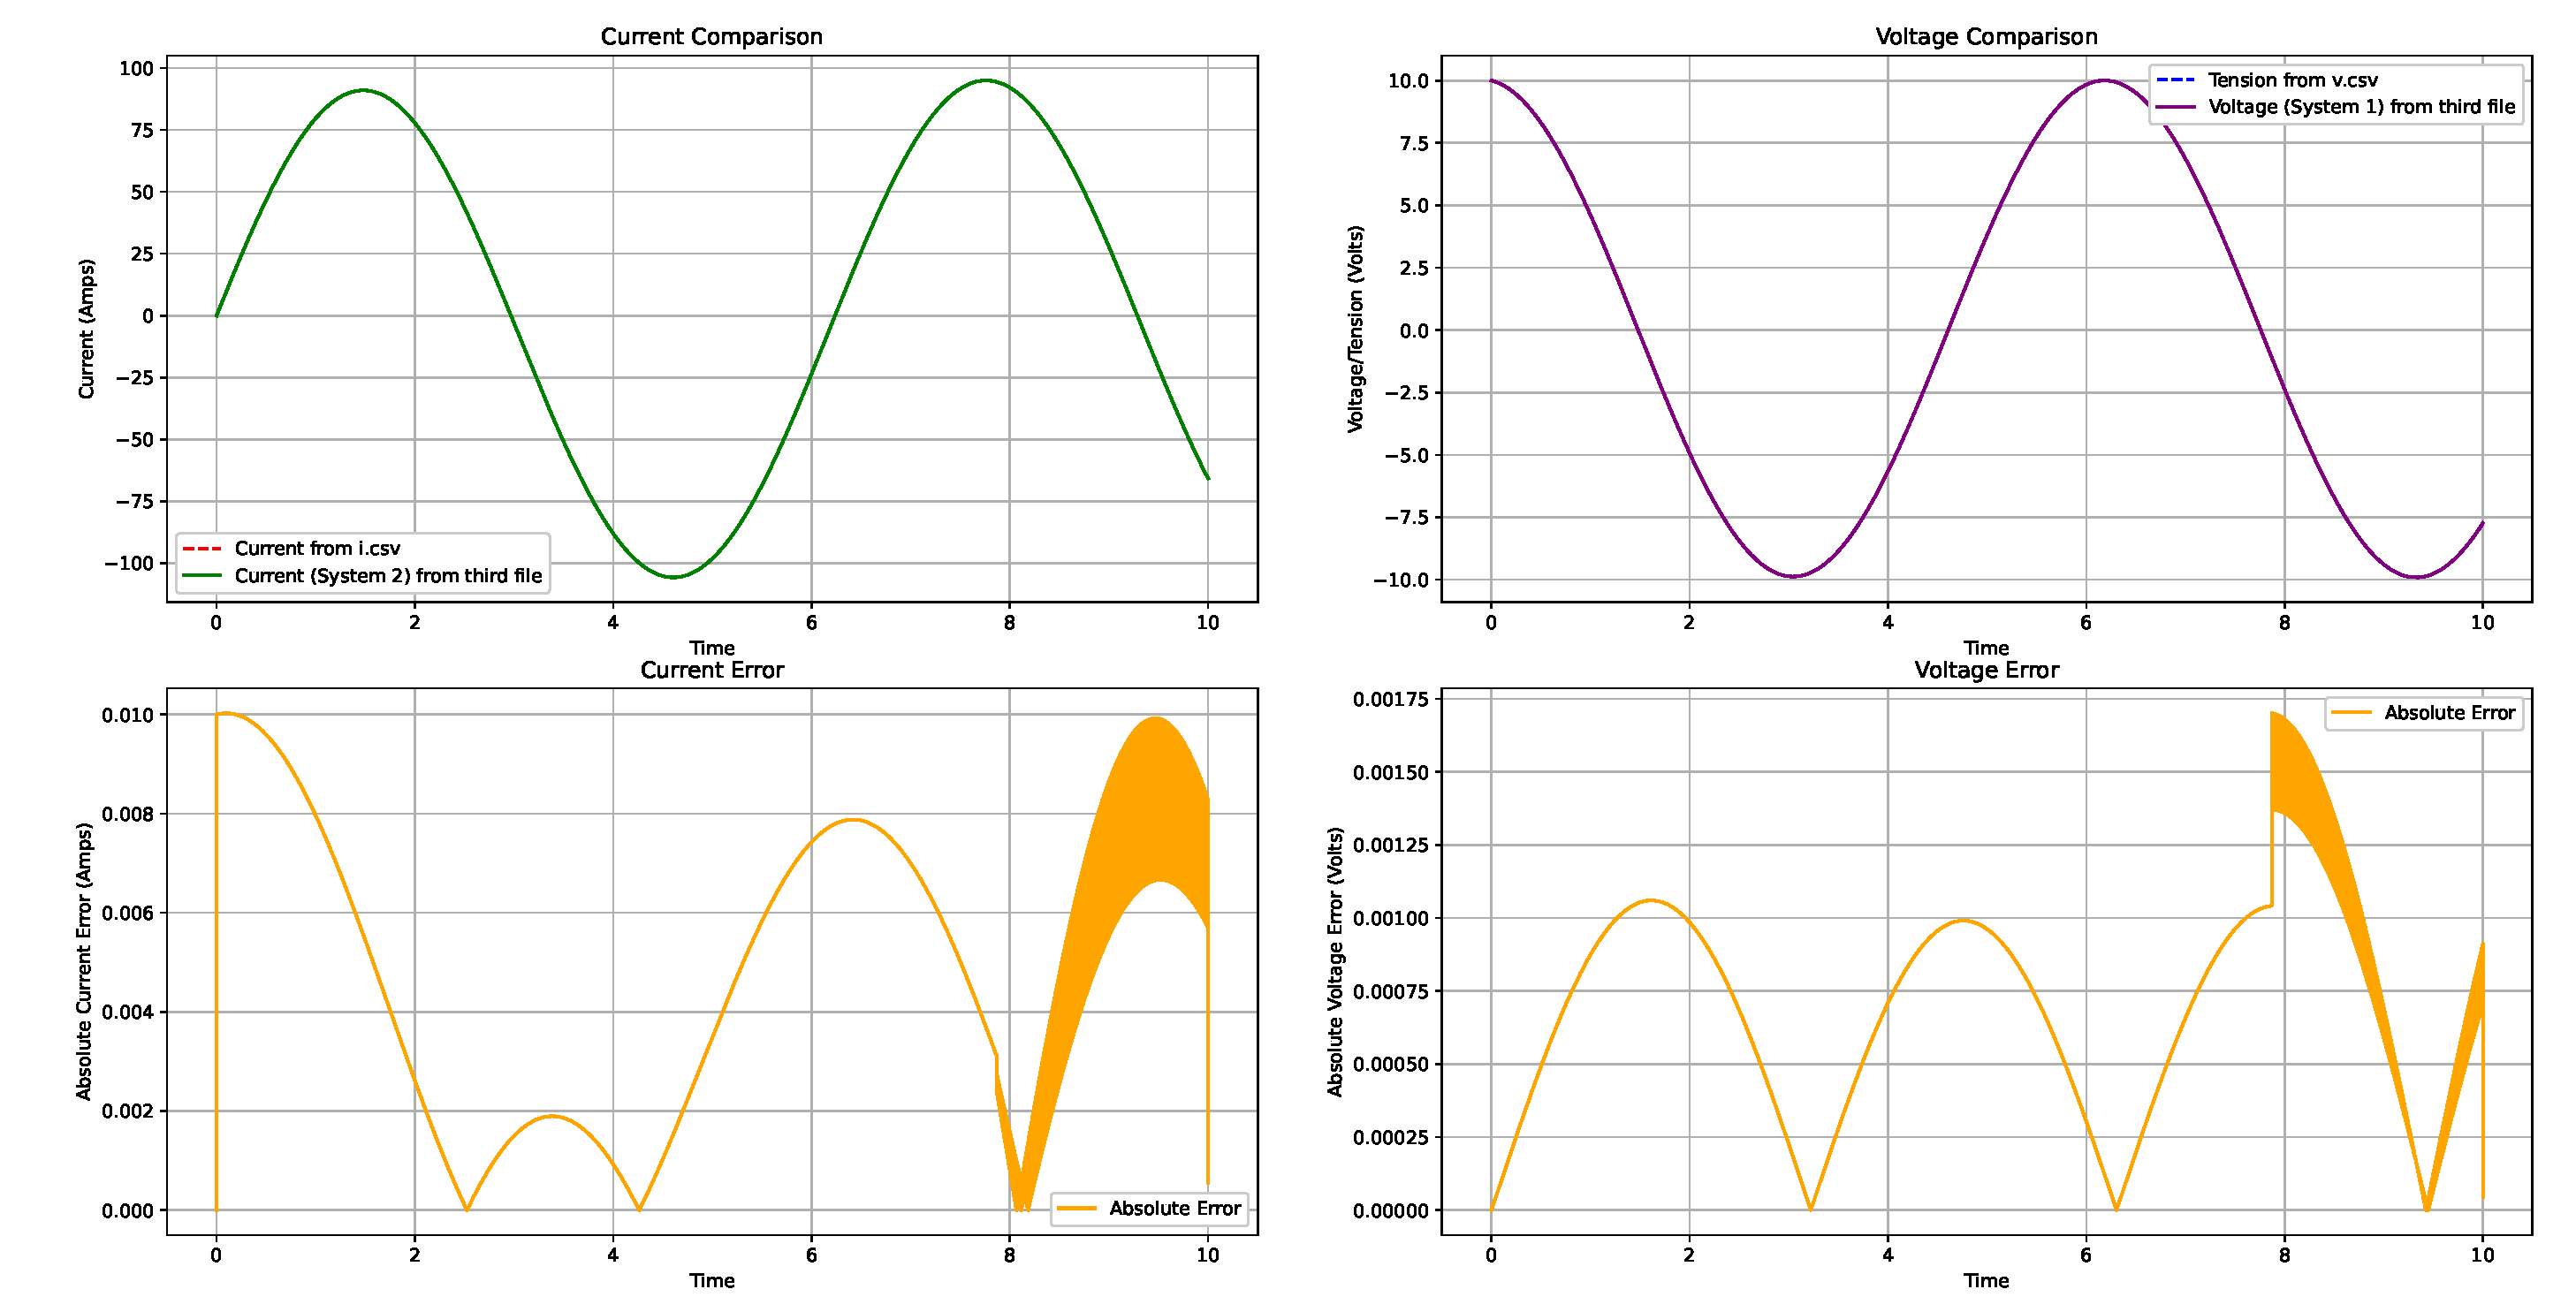
\includegraphics[width =\textwidth]{RLschwarz.eps}
    \caption{Comparaison de l'orchestrateur Aitken-Schwarz avec une simulation monolithique du circuit RL}
    \label{fig:26}
\end{figure}

On a aussi testé la méthode sur un circuit RL : 
\begin{equation}
    V_0 \cos(t) = RI + L \frac{dI}{dt}
\end{equation}
Où le circuit est divisé en deux FMUs : l'un comprend la source de tension et la résistance, et l'autre contient une bobine. Les résultats de cette configuration sont exposés dans la figure \ref{fig:26}. Les variables portant le suffixe (System) proviennent de la co-simulation. L'erreur absolue entre les résultats de la co-simulation et ceux de la simulation monolithique est également présentée.

\begin{figure}[hbt!]
    \centering
    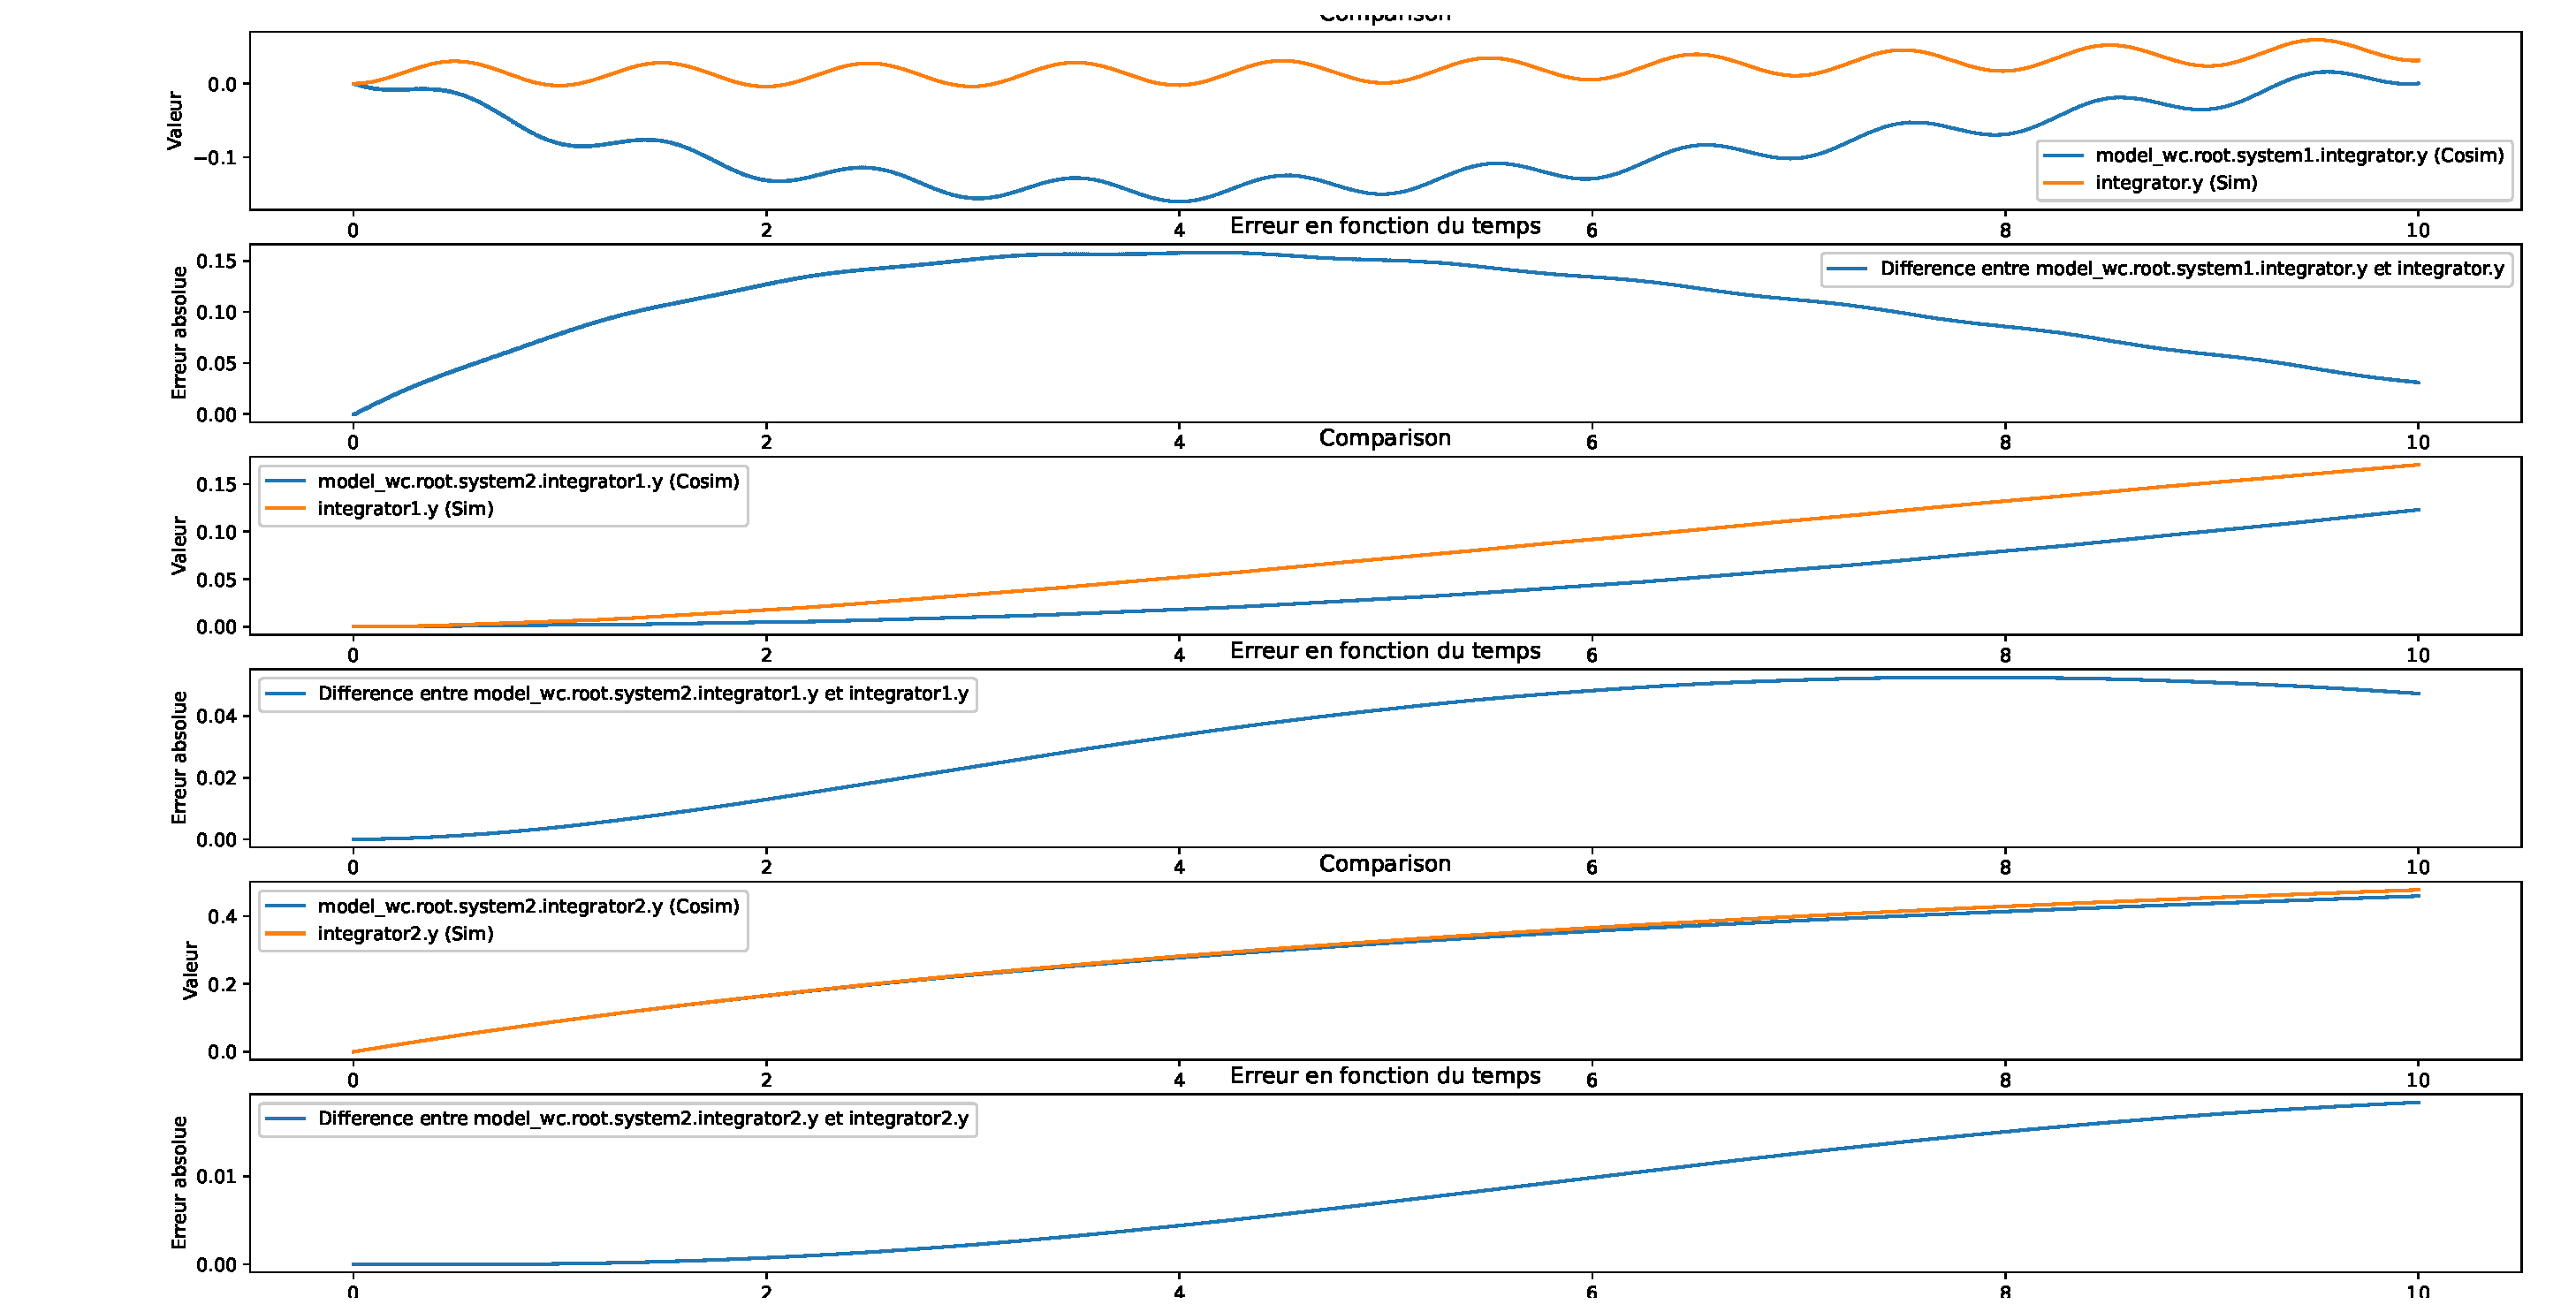
\includegraphics[width =\textwidth]{chainevolOMS.eps}
    \caption{Comparaison de l'orchestrateur Aitken-Schwarz avec une simulation monolithique du modèle \ref{fig:29}}
    \label{fig:27}
\end{figure}

\begin{figure}[hbt!]
    \centering
    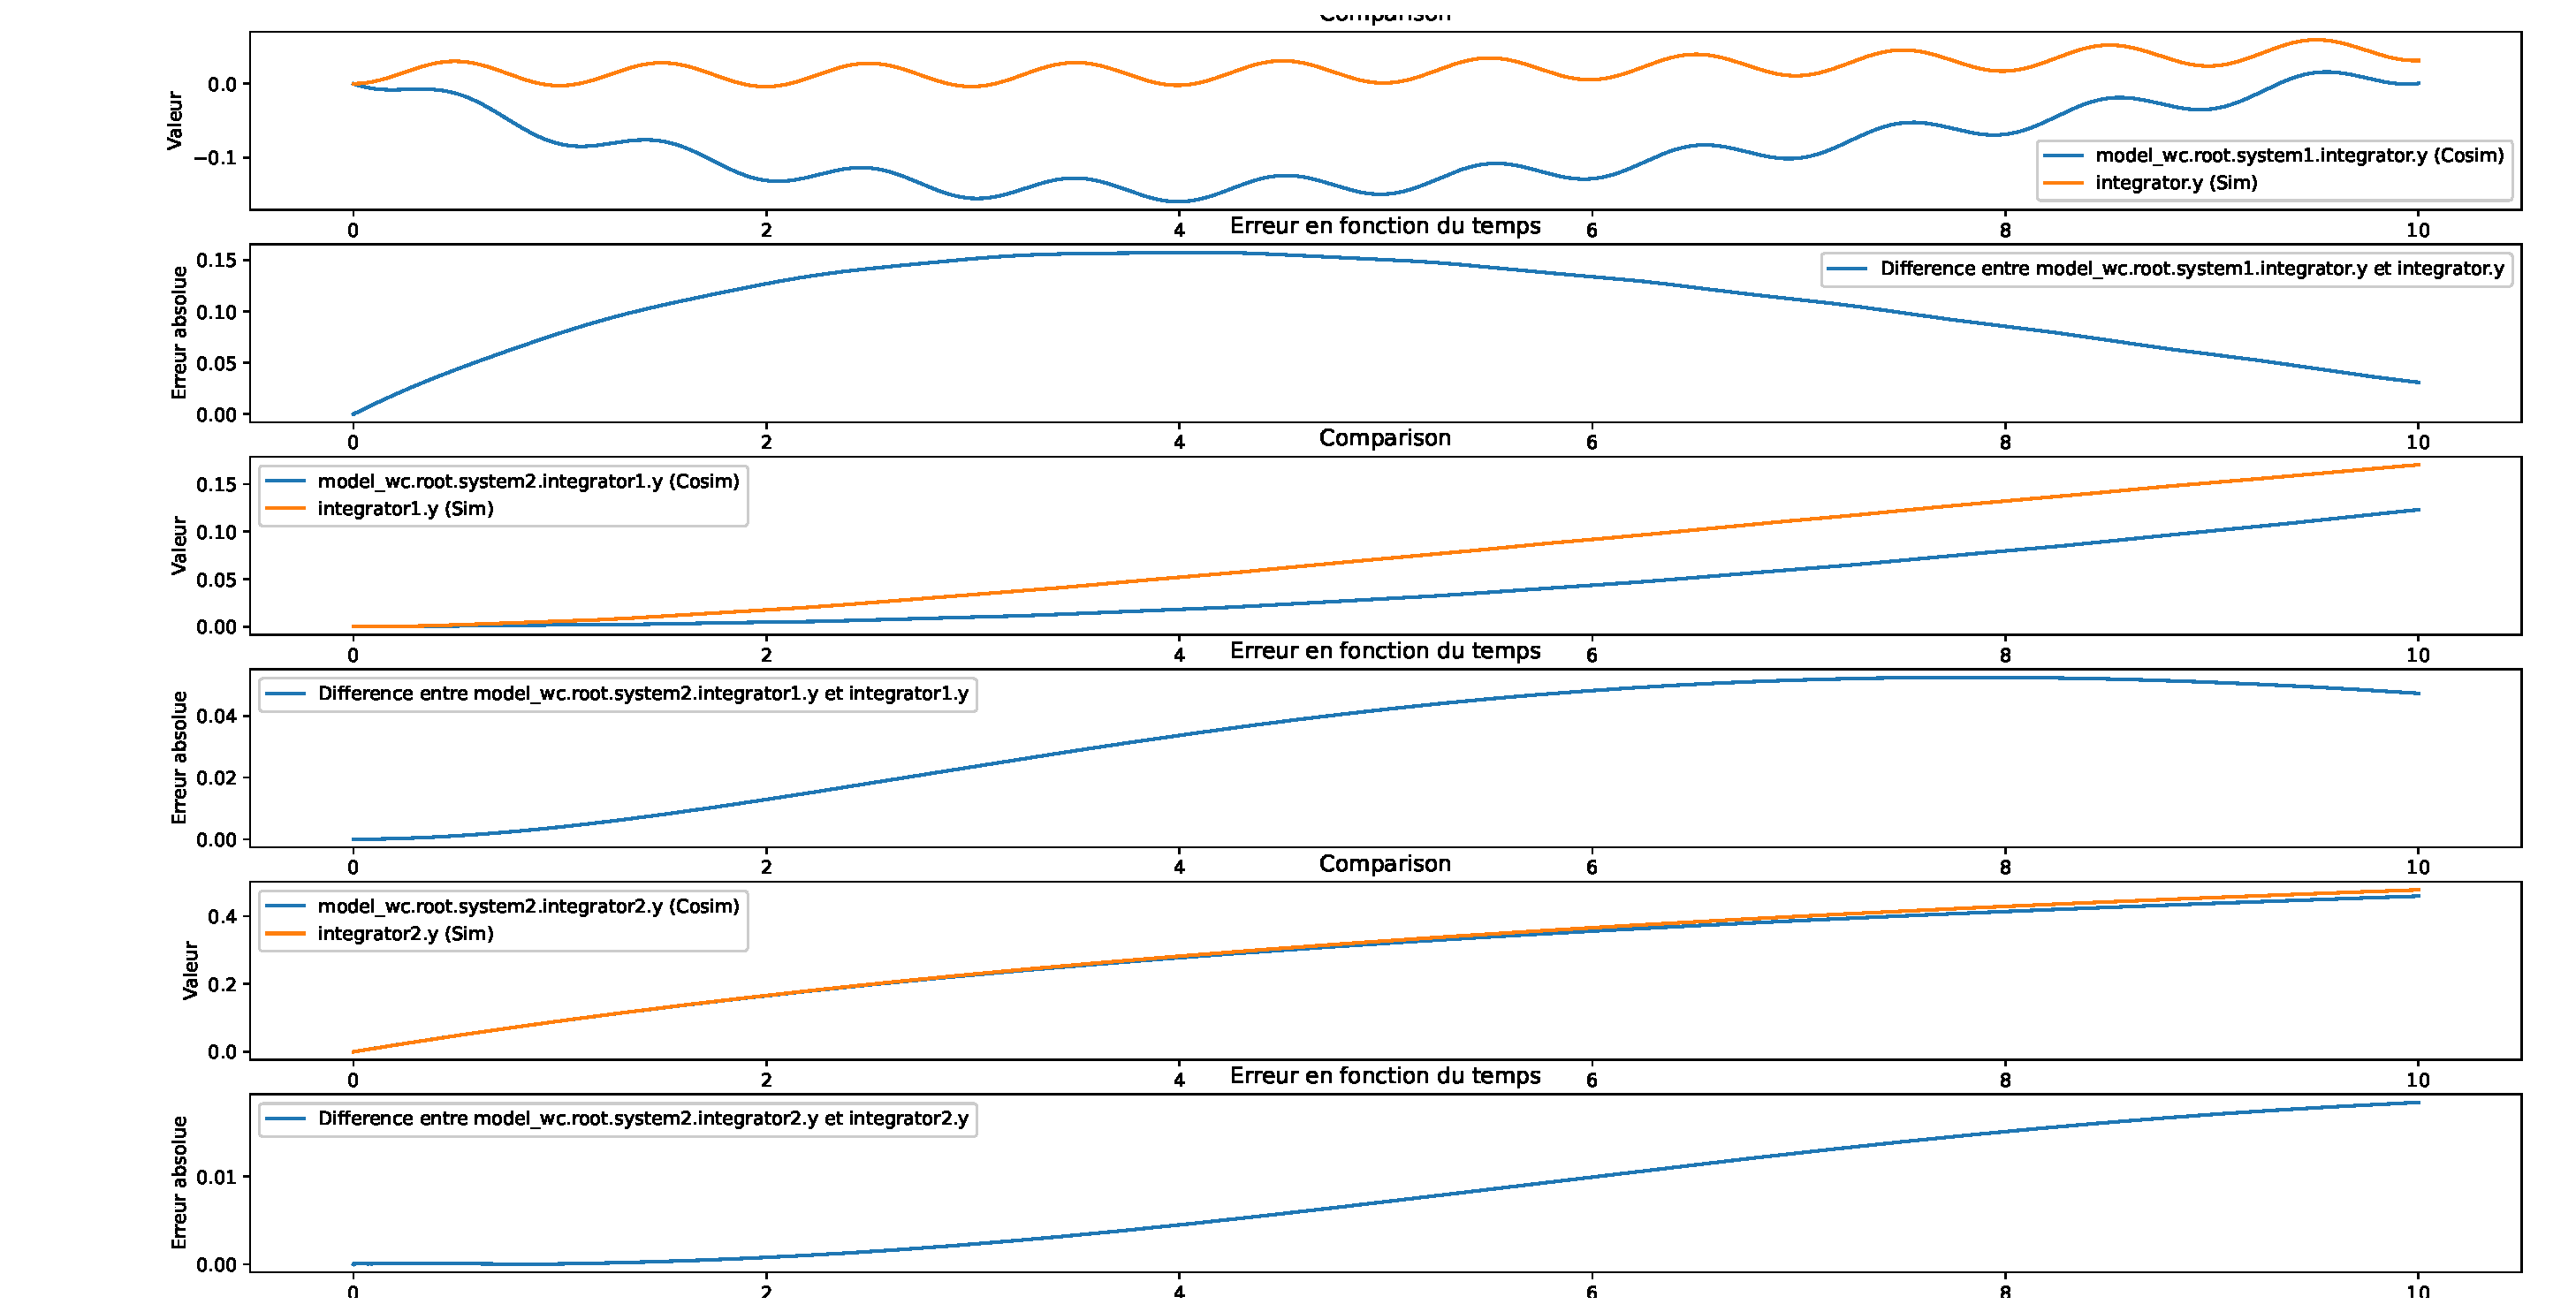
\includegraphics[width =\textwidth]{chainevolschwarz.eps}
    \caption{Comparaison de l'orchestrateur d'OMS avec une simulation monolithique du modèle \ref{fig:29}}
    \label{fig:28}
\end{figure}

\begin{figure}[hbt!]
    \centering
    \begin{minipage}[b]{0.4\textwidth}
        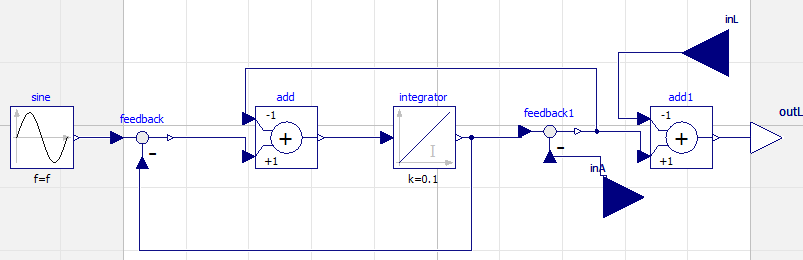
\includegraphics[width=\textwidth]{chainevolL.png}
    \end{minipage}
    \begin{minipage}[b]{0.4\textwidth}
      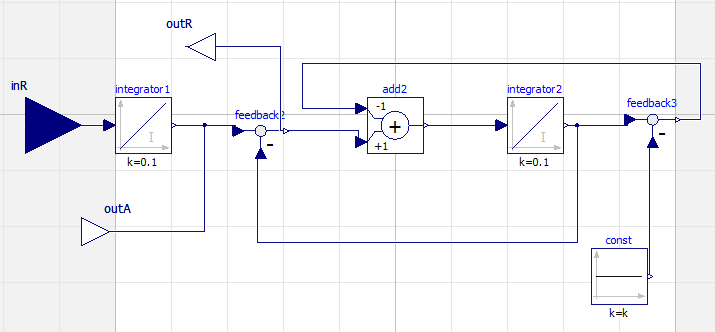
\includegraphics[width=\textwidth]{chainevolR.png}
  \end{minipage}
  \caption{Modèles utilisés dans la co-simulation d'une chaîne de contrôle de signal}
  \label{fig:29}
  \end{figure}
\newpage

La figure \ref{fig:29} représente une chaîne de traitement d'un signal, que l'on a découpée et exportée en FMUs, afin de comparer la simulation monolithique à la co-simulation avec la méthode d'Aitken-Schwarz dans \ref{fig:27} et l'orchestrateur à pas fixe d'OMS dans \ref{fig:28}.

\begin{figure}[hbt!]
    \centering
    \begin{minipage}[b]{0.45\textwidth}
        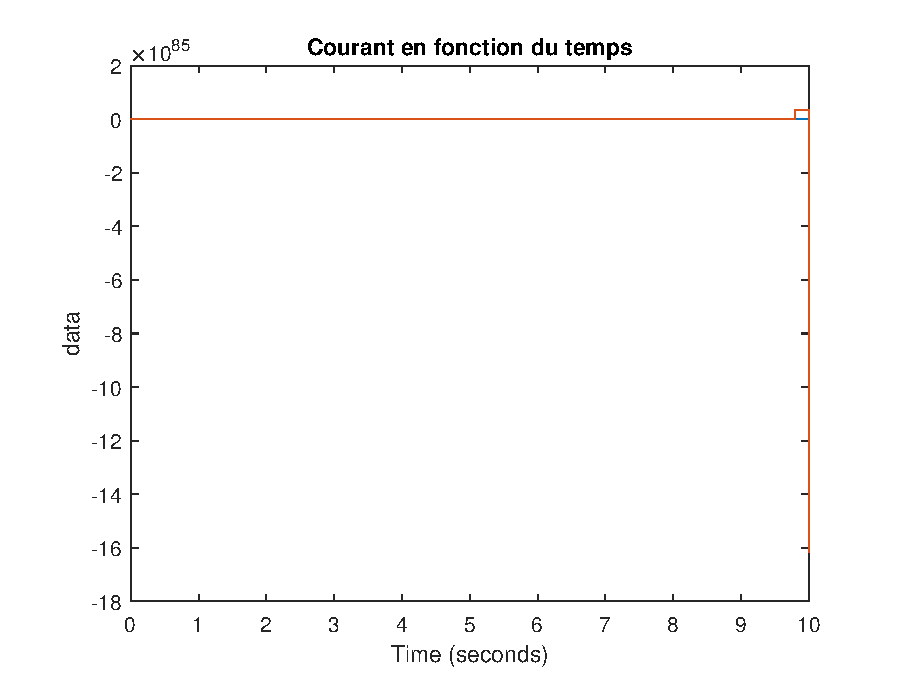
\includegraphics[width=\textwidth]{RL.eps}
        \caption{Résultats de la co-simulation du circuit RL sur Simulink}

    \end{minipage}
    \begin{minipage}[b]{0.45\textwidth}
      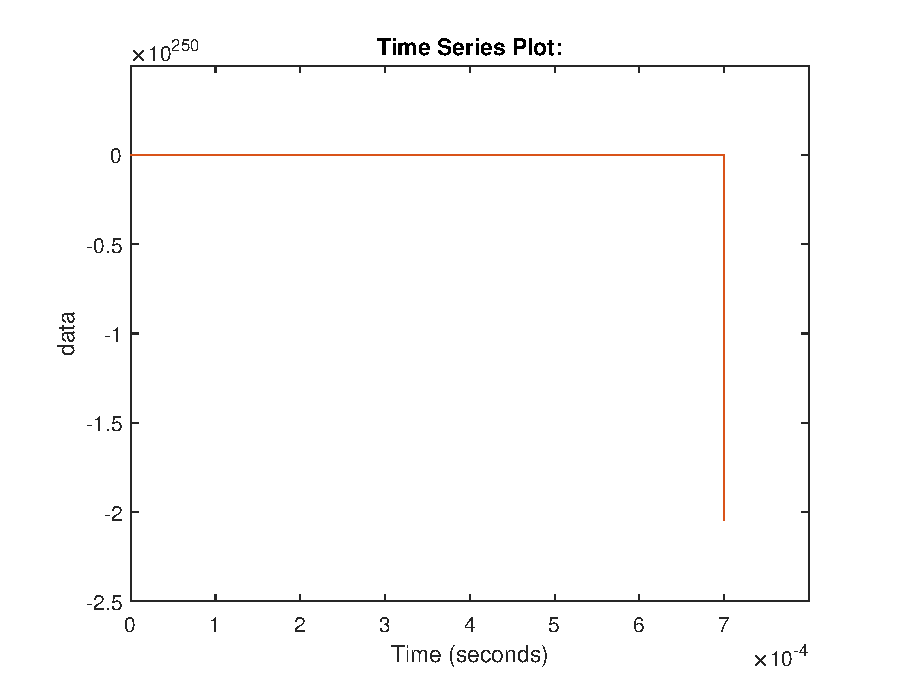
\includegraphics[width=\textwidth]{differenceAmplifier.eps}
      \caption{Résultats de la co-simulation de l'amplificateur différentiel \ref{fig:21} }
  \end{minipage}
  \label{fig:31}
  \end{figure}
  La figure \ref{fig:31} illustre les résultats obtenus via la co-simulation utilisant l'orchestrateur de SIMULINK. Cet orchestrateur appartient à la catégorie des algorithmes qui ne recourent pas à des fonctionnalités avancées telles que la capacité de faire un rollback, la modification des dérivées ou la sérialisation des données.

\section{Conclusion et perspectives}
En conclusion de ce chapitre, nous avons exploré les plateformes de co-simulation et les algorithmes d'orchestration, mettant en lumière leur importance cruciale dans la gestion efficace et précise des simulations complexes. À travers une analyse comparative des plateformes open source disponibles, nous avons identifié OMSimulator comme étant particulièrement adapté à nos besoins en raison de sa robustesse, sa documentation exhaustive, et sa capacité à intégrer diverses configurations de co-simulation. L'implémentation de l'algorithme d'orchestration Aitken-Schwarz a démontré des avantages significatifs en termes de gestion des erreurs et de la stabilité des simulations, confirmant ainsi l'efficacité de notre approche sélectionnée. Effectivement, on observe que l'erreur présentée dans la figure \ref{fig:24} atteint une magnitude de $0.14$, alors que dans la figure \ref{fig:25}, elle est réduite à $0.012$. Cette réduction montre que la méthode Aitken-Schwarz améliore les performances de la simulation par un facteur de 10 par rapport à la méthode par défaut d'OMS. Par ailleurs, dans la figure \ref{fig:26}, l'erreur est de $1.05\cdot 10^{-4}$. Cependant, la figure \ref{fig:31} révèle que la co-simulation a divergé, en raison de la présence d'une boucle algébrique (DAE), illustrant ainsi les avantages significatifs de la méthode Aitken-Schwarz. Pourtant, comme remarqué dans les figures \ref{fig:27}, \ref{fig:28}, les deux orchestrateurs ne parviennent pas à égaler les performances de la simulation monolithique. Cette limitation est attribuable au caractère très dynamique du système et à la manière dont il a été segmenté. En effet, le système comprend plusieurs intégrateurs, soulignant ainsi la nécessité d'adopter une méthode prédictive pour améliorer la précision de la co-simulation.
%\chapter{Compréhension des scènes RADAR}\label{chap:4}
\section{Introduction}
La compréhension des scènes RADAR est un sujet qui en est à ses débuts, mais avec un grand potentiel or le radar compense les points faibles des autres capteurs. Les données RADAR sont sous formes d'un tenseur RAD, on a traité dans le chapitre précédent le problème d'annotation de ces données ainsi que les différents types d'annotations présenté. L'annotation à boite englobante n'est pas assez convenable pour ce type de tâches, car les données Radar sont assez différents que les images issue d'une caméra, les points réfléchit par les objets sont assez distants et les signatures des objets sont assez distincts, d'où l'utilisation de la segmentation sémantique dans ce projet. 

Dans ce chapitre, on introduit une méthode d'apprentissage supervisé profonde pour la segmentation sémantique des données RADAR, on montre l'architecture du modèle ainsi que les fonctions de pertes adaptées pour les représentations du tenseur RAD.
\section{La segmentation sémantique des scènes RADAR}
\subsection{Exemples des modèles}
Dans cette section on présente plusieurs méthodes utilisé pour la segmentation sémantique dans la littérature, ces derniers sont choisis car il existe des mesures de leurs performances dans le cas des données RADAR. 
\begin{enumerate}
  \item Architectures destiné aux images : 
  \begin{itemize}
    \item Réseaux entièrement convolutifs (FCN) : Dans \cite{46}, Long et al. proposent FCN, une architecture totalement basé sur les couches convolutifs (Convolution, compression et après convolution transposé), la représentation finale est traité une couche convolutif unidimensionnelle avec la fonction d'activation Softmax, afin de classifier chaque pixel, plusieurs versions de cette architecture est utilisé sur les données RADAR, l'architecture FCN-8s présente les meilleurs résultats. 
    \item U-Net : L'architecture U-Net \cite{47} est composé de voies de compression et décompression à profondeur égale. Ce modèle est utilisé à l'origine pour les images médicales, il est particulièrement bien adapté à la segmentation des petits objets.
    \item DeepLabv3+ \cite{48} est un modèle basé sur le prince des auto-encodeurs pour la segmentation des images naturels. Les auteurs proposent la couche pyramides spatiales à convolutions dilatées ASPP (qu'on va détailler dans la sous-section suivante).
    \item Dans \cite{32} Zhang et al., proposent une architecture qui combine l'architecture ResNet-101 \cite{51} comme extracteur de caractéristiques (Backbone) et une tête basé sur YOLO (décodage) \cite{26}, on détaillera brièvement cette architecture dans la sous-section prochaine.
  \end{itemize}
  \item Architectures destiné aux données RADAR : 
  \begin{itemize}
    \item Gao et al. \cite{49} proposent une architecture à multiple perspectives des données RADAR (RAMP-CNN), pour la détection des objets dans la représentation RA. Les vues 2D extraites du tenseur RAD, sont traité par des auto-encodeurs à convolutions tri-dimensionnelles. RAMP-CNN atteints des performances intéressantes.
    \item Arthur et al. \cite{50} proposent TMVA-NET, une architectures qui rassemblent les qualités de traitement dans la base temporaire présenté dans RAMP-CNN \cite{49}, en plus l'avantage de la couche pyramides spatiales à convolutions dilatées ASPP utilisé dans DeepLabv3+ par l'équipe des chercheurs de google \cite{48}. Ainsi les résultats présenté par cette architecture présente plus ou moins l'état de l'art à un nombre de paramètres inférieure aux autres architectures.
  \end{itemize}
\end{enumerate}
\subsection{Méthodes et outils}
\textbf{Convolution :} Mathématiquement, une convolution est une fonction d'intégration qui exprime le degré de recouvrement d'une fonction g lorsqu'elle est décalée par rapport à une autre fonction f.
Intuitivement, une convolution agit comme un mixeur qui mélange une fonction avec une autre pour réduire l'espace de données tout en préservant l'information. Il existes plusieurs types de couches convolutifs; 

\textbf{Les couches de convolution 1D} sont utilisés pour extraire les sous-séquences 1D locales des séquences d'entrée et identifier les motifs locaux dans la fenêtre de convolution.
\begin{figure}[hbt!]
  \centering
  \includegraphics[width=0.6\textwidth]{tikzconv.pdf}
\end{figure}

\textbf{Les couches de convolution 2D}, l'idée principale est que le filtre convolutif se déplace dans deux directions (x,y) pour calculer les caractéristiques de faible dimension à partir des données de l'image. La forme de sortie est également une matrice à 2 dimensions.
\begin{figure}[hbt!]
  \centering
  \includegraphics[width=0.7\textwidth]{tikzconv2d.pdf}
\end{figure}

\textbf{Les couches de convolutions 3D} appliquent un filtre tri-dimensionnel qui se déplace dans 3-axes  (x,y,z) afin de calculer les représentations des caractéristiques de bas niveau.\footnote{Dans notre cas on force une dimension temporelle à nos données, en empilant 5 vues (RD ou RA) dans le troisième axe.}
\begin{figure}[hbt!]
  \centering
  \includegraphics[width=0.6\textwidth]{3dconv.jpg}
\end{figure}

\textbf{Convolution ponctuelle dilatée} : La convolution ponctuelle permet d’obtenir une convolution dilatée (ou “à trous”, atrous convolution en anglais) en ajoutant un taux de dilatation r, qui définit l'espacement entre les cellules du noyau. Celui-ci permet d'augmenter la taille du noyau, donc le champ récepteur, sans avoir à traiter trop de pixels. Des gains de vitesse considérables sans perte de précision en résultent.
\begin{figure}[hbt!]
  \centering
  \includegraphics[width=0.6\textwidth]{atrous_convolution.png}
\end{figure}

\textbf{Convolution transposé 2D} : (par abus de language on dit "déconvolution"); Contrairement à la convolution normale qui réduit les éléments d'entrée via le noyau, la convolution transposée diffuse les éléments d'entrée via le noyau, produisant ainsi une sortie plus grande que l'entrée. 
\begin{figure}[hbt!]
  \centering
  \includegraphics[width=0.8\textwidth]{transconv.pdf}
\end{figure}

\textbf{Max pooling 2D}: La mise en commun maximale (Max Pooling) est une opération de mise en commun qui calcule la valeur maximale des parcelles d'une carte d'entités et l'utilise pour créer une carte d'entités sous-échantillonnée (mise en commun). Elle est généralement utilisée après une couche convolutive. Il ajoute une petite invariance de traduction, ce qui signifie qu'une petite translation de l'image n'affecte pas de manière significative les valeurs de la plupart des sorties regroupées.
\begin{figure}[hbt!]
  \centering
  \includegraphics[width=0.6\textwidth]{maxpool.png}
\end{figure}


\textbf{Couche pyramides spatiales à convolutions dilatées ASPP :} Comme on a vue dans la partie concernant la \textbf{Convolution ponctuelle dilatée}, cette opération réduit dramatiquement le taux de calcul on tirant un ensemble assez bien de caractéristiques, l'idée de l'ASPP est de combiner plusieurs couches de convolution ponctuelle à différents dilations, pour capturer des informations contextuelles à plusieurs échelles. En utilisant différents taux de dilatation, le ASPP permet au réseau d'avoir accès à des informations à différentes échelles, ce qui est crucial pour capturer des objets de différentes tailles dans une image. Cela permet au réseau d'avoir une compréhension plus complète de la scène. Il a été démontré que l'ASPP améliore la précision de la segmentation dans diverses tâches de compréhension d'images. En capturant des informations contextuelles multi-échelles et en augmentant le champ réceptif, l'ASPP permet au réseau de mieux distinguer les différents objets et d'attribuer avec précision des étiquettes de classe à chaque pixel. Cela peut conduire à des résultats de segmentation plus précis et plus détaillés. \cite{48}

\textbf{Auto-encodeurs (codeur-décodeur)}:Les réseaux codeur-décodeur ont été appliqués avec succès à de nombreuses tâches de vision par ordinateur, notamment l'estimation de la pose humaine \cite{52}, la détection d'objets et la segmentation sémantique. En général, les réseaux codeur-décodeur contiennent un module codeur qui réduit progressivement les cartes de caractéristiques et capture des informations sémantiques plus importantes, et un module décodeur qui récupère progressivement les informations spatiales. 

\begin{figure}[hbt!]
  \centering
  \begin{minipage}[b]{0.5\textwidth}
      \includegraphics[width=\textwidth]{ASPP.png}
      \caption{Architecture avec ASPP}
  \end{minipage}
  \begin{minipage}[b]{0.45\textwidth}
    \includegraphics[width=\textwidth]{encoderdecoder.png}
    \caption{Un auto-encodeur}
\end{minipage}
\end{figure}
\subsection{L'architecture RAMP-CNN}\label{sec:423}
\begin{figure}[hbt!]
  \centering
  \includegraphics[width=\textwidth]{RAMP.png}
  \caption{Le modèle RAMP-CNN \cite{49}}
  \label{fig:43}
\end{figure}
Comme montré dans la figure \ref{fig:43}, le modèle implémente 3 auto-encodeurs (CAE) qui servent à tirer les caractéristiques des trois Représentation RA, RD, AD. Un module de fusion des sorties de chaque décodeur afin de combiner les caractéristiques dans une représentation qui ressemble à la vue Portée Angle (RA). Le premier CAE traite les séquences des vues RA avec des couches de convolution 3D et des couches de convolution transposées. Ces opérations de convolution 3D tirent parti non seulement des motifs spatiaux de l'objet dans une seule image, mais aussi des informations temporelles qui contient le changement des motifs spatiaux entre les images. Certains aspects des motifs spatiaux, comme la distribution de l'intensité de la réflexion, contribuent directement à la reconnaissance des objets, par exemple, les objets de grande taille (véhicules) contiennent plus de réflecteurs plus puissants que les petits objets.
\subsection{L'architecture DeepLabv3+}
\begin{figure}[hbt!]
  \centering
  \includegraphics[width=0.7\textwidth]{deeplab.png}
  \caption{Module ASPP \cite{48}}
\end{figure}
Le module ASPP consiste en : 
\begin{itemize}
  \item une convolution 1×1 pour garder l'information de la carte de caractéristique utile pour que le réseau discrimine certaines structures ; de trois convolutions 3×3 en parallèle avec des taux de dilatation respectivement égaux à 6, 12, 18, et un pas de sortie égal à 16 permettant de capturer le contexte à différentes échelles, ces valeurs sont les meilleurs trouvés empiriquement dans l’article \cite{53}.
  \item un sous-échantillonnage de la carte pour lisser les contours et mettre en avant des caractéristiques larges.
  \item la concaténation des cartes de caractéristiques résultantes.
  \item une convolution 1×1 de réduction du nombre de cartes de caractéristiques à 256.
  \item enfin, un sur-échantillonnage de la taille de la carte de caractéristique à celle de l’image finale.
\end{itemize}
\newpage
\subsection{L'architecture RadarResNet}

\begin{figure}[hbt!]
  \centering
  \includegraphics[width=\textwidth]{Raddet.png}
  \caption{Architecture RadarResNet \cite{32}}
\end{figure}

Le modèle est une adaptation du ResNet-101 \cite{50} et YOLO \cite{26} pour les données RADAR, en plus les auteurs introduits plusieurs modules d'améliorations tel que les couches d'Auto-Attention qui améliorent les performances des réseaux profonds comme démontré dans \cite{54}, et obtient des résultats intéressantes sur leurs bases de données RADDet \cite{32}.

\subsection{L'architecture TMVA-Net}
\begin{figure}[hbt!]
  \centering
  \includegraphics[width=0.8\textwidth]{teaser_schema.png}
  \caption{Réseau temporel multi-vues avec modules ASPP (TMVA-Net) \cite{50} }
  \label{fig:46}
\end{figure}
Dans \cite{50}, Arthur et al. développent trois architectures de réseaux neuronaux légers, qui sont conçues spécifiquement pour la segmentation sémantique des radars à vues multiples, et leur idée générale est illustrée à la figure \ref{fig:46}. Ils traitent les vues radar avec des encodeurs spécialisés utilisant une pile temporelle comme entrée. 
Différents décodeurs prévoient des cartes de segmentation sémantique pour chaque vue de sortie à partir des cartes de caractéristiques fusionnées dans un espace latent partagé.
Par conséquent, il existe des composants de réseau spécifiques pour chaque vue, ainsi qu'un nombre raisonnable de paramètres dans l'ensemble.

Or notre modèle partagent les points forts de chacune de ces architectures, on détaillera ces points lors de la présentation de notre architecture dans la prochaine section.

\section{L'architecture proposé}
\begin{figure}[hbt!]
  \centering
  \includegraphics[width=\textwidth]{tikz.pdf}
  \caption{Réseau temporel avec modules ASPP pour la segmentation des vues RA et RD}
  \label{fig:your_label}
  \end{figure}
On propose une architecture basé sur un double codeur-décodeur, or chaque couple est destiné pour une vue RADAR spécifique (RD ou RA), et qui prédis simultanément la segmentation de ces deux vues. On implémente deux couches de convolutions 3D, comme expliqué dans la sous-section \ref{sec:423}, le domaine temporelle est très intéressant dans notre cas, or les tâches spatiales que chaque objet laisse peuvent aider à bien les classifier. Ainsi la forme des données RA est (256x256x5) et RD (256x64x5).

On élimine la vue AD car on cherche à diminuer le nombre des paramètres entraînable du modèle, en plus qu'on peut la déduire directement des deux vues RD et RA et on se restreint à utiliser deux blocs de convolution 3D, au lieu de toutes l'architecture, car ces derniers demande un nombre assez grand de paramètres.

Après les deux blocs de convolution 3D, leurs normalisation par lots et couches d'activations, on introduit une couche de sous-échantillonnage (Max pooling) selon l'axe de portée et angle (l'axe doppler est déjà petit, on le laisse comme il est). Les cartes de caractéristiques obtenues sont traité par des couches de convolution 1D et empilés dans un espace latent commun. Les caractéristiques de l'espace latent partagé sont ensuite traitées avec des couches de convolution 1D et utilisées avec les caractéristiques à multi-échelles générés par les modules ASPP comme entrée de chaque décodeur. Deux décodeurs prédisent respectivement les cartes de segmentation sémantique RD et RA. Chacun est composé de deux blocs avec deux séquences de couches de convolution, de normalisation par lots et d'activation. L'échantillonnage ascendant entre les blocs est réalisé par des convolutions transposés. Une convolution 1D finale combine les sorties de chaque décodeur pour générer K cartes de caractéristiques, où K est le nombre de classes. Une opération de softmax est ensuite appliquée par pixel aux K cartes de caractéristiques pour générer des masques doux.
\section{Fonctions de pertes}
L'objectif de la segmentation sémantique RADAR multi-vues est de segmenter simultanément de nombreuses vues du tenseur RAD agrégé. Il est évident qu'un certain degré de cohérence doit être maintenu entre les vues segmentées, car les éléments que nous voulons détecter sont visibles dans les différentes perspectives RADAR. Par exemple, un cycliste ne doit pas être représenté dans une vue alors qu'un piéton l'est dans une autre. Pour que les prédictions du modèle restent cohérentes, une perte de cohérence (Coherence Loss, CoL) est mise en œuvre.
Dans \cite{25}, les auteurs démontrent la procédure de calcul de cette fonction. Dans cette section on détaillera tous les fonctions utilisé dans ce projet.

On note $f_\theta (x) = p $ un modèle de segmentation à paramètres $\theta$, entrée $x$ et sortie $p$. Entraîner le modèle correspond à minimiser une fonction de pertes décrivant le modèle. Or notre modèle est à principe de multi-vues, l'entrée est sous la forme de $x=(x^{RA}, x^{RD})$, et la sortie est un masque lisse $p = (p^{RA}, p^{RD})$\footnote{$p^{RD}\in [0,1]^{B_R\cdot B_A\cdot K}$ avec $B_R$, $B_D$ les dimensions de la matrice RD et $K=4$ le nombre de classes à distinguer (Arriè4re-plan, voiture, cycliste, piéton). } pour les deux vues RD et RA. 

\textcolor{blue}{\textbf{Cohérence}} : Soit $(p^{RA},p^{RD}) $ les cartes de segmentation prédites par le modèle. Ces deux matrices sont agrégé par l'opérateur $max(.)$ au long de l'axe non partagé (Angle ou Doppler). Les deux matrices résultantes noté $\tilde{p}^{RA}$ et $\tilde{p}^{RD}$,comprennent la plus grande probabilité de chaque point de l'axe Portée pour chaque classe, c-à-d ils indiquent si le modèle prédit une forte probabilité d'observer une catégorie à une distance donnée.
La perte de cohérence est l'erreur quadratique moyenne entre les vecteurs de probabilité maximale (portée), l'extension de cette opération pour le cas des matrices est la norme de Frobenius (voire Annexe \ref{sec:B5}). Le but de cette fonction est d'encourager le modèle à prédire les grandes probabilité à la même distance et pour la même classe pour les deux vues. 
La fonction de pertes à cohérence CoL dans l'interval [0,1] est définie comme : 
\begin{equation}
  \mathcal{L}_{CoL} (p^{RA},p^{RD})= \frac{1}{\mathcal{B}_R \cdot K} \Vert\tilde{p}^{RA}-\tilde{p}^{RD} \Vert_F ^2
\end{equation}
Avec $\Vert \cdot \Vert_F $ la norme de Frobenius.
\begin{figure}[hbt!]
  \centering
  \includegraphics[width=0.7\textwidth]{CoL.png}
  \caption{Méthode de calcul des pertes de cohérence.\cite{25}}
\end{figure}

\textcolor{blue}{\textbf{Dice}} : Une autre fonction de perte pour les tâches de segmentation d'images est basée sur le coefficient de Dice, qui est essentiellement une mesure du superposition entre deux échantillons. Cette mesure varie de 0 à 1, un coefficient de Dice de 1 indiquant une superposition parfaite et complète. Le coefficient Dice \cite{55} a été développé à l'origine pour les données binaires et peut être calculé comme suit :
\begin{equation}
  Dice=\frac{2\vert A \cap B \vert }{\vert A \vert + \vert B \vert}
\end{equation}
Où $\vert A \cap B \vert$ représente les éléments communs entre les ensembles A et B, $\vert A \vert$ représente le nombre d'éléments de l'ensemble A (et de même pour l'ensemble B).

Dans le cas de l'évaluation d'un coefficient de Dice sur des masques de segmentation prédits, nous pouvons faire l'approximation de $\vert A \cap B \vert$  en multiplication par éléments entre le masque de prédiction et le masque cible, puis faire la somme de la matrice résultante.
\begin{figure}[hbt!]
  \centering
  \includegraphics[width=\textwidth]{DICEnom.png}
\end{figure}

Pour quantifier $\vert A \vert$ et $\vert B \vert$, certains chercheurs utilisent la somme simple tandis que d'autres préfèrent utiliser la somme quadratique pour ce calcul. En outre, il y a un 2 au numérateur dans le calcul du coefficient de Dice car notre dénominateur "compte deux fois" les éléments communs aux deux ensembles. Afin de formuler une fonction de pertes qui peut être minimisée, nous utiliserons simplement $1-Dice$. Cette fonction de pertes est connue sous le nom de pertes de Dice douce car nous utilisons directement les probabilités prédites au lieu de les seuiller et de les convertir en un masque binaire. Le coefficient devient : 

\begin{equation}
  Dice = \frac{2\sum_{pixels}y_{v}y_{p}}{\sum_{pixels}y_{v}^2 + \sum_{pixels}y_{p}^2}
\end{equation}
Avec $y_v$ les bases de vérités, $y_p$ les prédictions du modèle. On effectue ce calcul pour chaque classe d'objet et on prend la moyenne, ainsi la fonction de pertes Dice est formulé comme suivant : 

\begin{equation}
\mathcal{L}_{SDice} = \frac{1}{K} \sum_{k=1}^{K} \left[ 1 - \frac{2\sum_{(m,n)}y[m,n,k]p[m,n,k]}{\sum_{(m,n)}y[m,n,k]^2+\sum_{(m,n)}p[m,n,k]^2}\right]
\end{equation}\label{eqn:44}

Où $y\in \{0,1\}^{B_M\cdot B_N \cdot K}$ la base de vérité, $f_\theta (x) = p \in [0,1]^{B_M\cdot B_N \cdot K}$ la prédiction associé, avec $B_M\cdot B_N $ les dimensions de la vue x. 

\textcolor{blue}{\textbf{Entropie croisée pondérée (wCE)}} : Les modèles de segmentation sémantique qui prédisent un score pour chaque classe à chaque pixel sont généralement formés en minimisant une fonction de perte à entropie croisée (CE). Cette perte n'est pas idéale pour les tâches de segmentation déséquilibrées telles que la segmentation sémantique RADAR, car le processus d'optimisation a tendance à se concentrer sur les classes les plus représentées. Dans le cas présent, le bruit d'arrière plan domine par rapport aux signatures des objets que nous souhaitons détecter. 

Dans le même espace que l'équation \ref{eqn:44}, on formule l'équation de pertes à entropie croisée pondérée : 
\begin{equation}
  \mathcal{L}_{wCE}(y,p)= -\frac{1}{K} \sum_{k=1}^{K} w_k \sum_{(m,n)}y[m,n,k] \log p[m,n,k]
\end{equation}
Avec $w_k$ des poids positives normalisées. Le poids $w_k$ est inversement proportionnel à la fréquence de la classe k dans l'ensemble de données d'entraînement. 
\begin{equation}
  w_k \varpropto (\sum_y \sum_{(m,n)} y[m,n,k])^{-1}
\end{equation}
En termes plus simples, le poids attribué à la classe k sera plus important s'il y a moins d'échantillons d'apprentissage avec cette classe particulière. En effet, le poids augmente pour compenser la rareté des échantillons et garantir que le modèle accorde plus d'attention à la classe la moins représentée au cours de la formation. Inversement, si une classe est plus abondante dans l'ensemble d'apprentissage, son poids sera plus faible car elle nécessite moins d'attention pendant l'apprentissage.

\textcolor{blue}{Pertes globales} : La perte d'entropie croisée (CE) est spécialisée dans la classification par pixel et ne tient pas compte des corrélations spatiales entre les prédictions. Le Dice est particulièrement efficace pour la segmentation des formes, mais il est difficile de l'optimiser en tant que fonction de perte unique en raison de sa formulation en gradient. Enfin, la CoL est utile lorsque ni la CE ni la Dice ne sont en mesure de tirer parti de la cohérence entre la prédiction des vues RD et RA. Pour combiner les différentes points forts de ces pertes, une perte globale est utilisé pour la segmentation à multi-vues :
\begin{equation}
  \mathcal{L} = \lambda_{wCE}(\mathcal{L}_{wCE}^{RA}+\mathcal{L}_{wCE}^{RD})+\lambda_{Dice}(\mathcal{L}_{Dice}^{RA}+\mathcal{L}_{Dice}^{RD})+\lambda_{CoL}\mathcal{L}_{CoL}
\end{equation}
$\lambda_{wCE}$, $\lambda_{Dice}$ et $\lambda_{CoL}$ sont des facteurs de pondération fixés à partir du travail du propriétaire de la base de données \cite{25}, or ils l'ont choisis d'une manière empirique.

\section{Expériences sur CARRADA}
\subsection{Procédure d'entraînement}
À cause des contraintes temporelles de ce projet, les résultats sont issues de l'ensemble des données CARRADA-VAL et le modèle est entraîné sur la partie CARRADA-Train, CARRADA-Test n'est pas utilisé dans cette version du rapport. À chaque instant de la séquence du RADAR, le tenseur RAD est traité comme montré dans la section \ref{sec:225}. 

Pour chaque image, un nombre d'images antérieure sont considéré dans la phase d'entraînement, or notre modèle à une entrée temporelle (Convolution 3D), on choisie 4 images (suffisant pour constater n'importe quel changement spatio-temporel).

On utilise l’Optimiseur ADAM\footnote{On utilise les paramètres recommandé ($\beta_1=0.9$, $\beta_2=0.999$ et $\epsilon = 10^{-8}$)} \cite{56}, qui est un algorithme d'optimisation couramment utilisé dans l'apprentissage automatique et l'apprentissage profond pour la formation des réseaux neuronaux. Il s'agit d'une extension de la méthode d'optimisation par descente stochastique du gradient (SGD) qui combine les avantages des taux d'apprentissage adaptatifs et des mises à jour basées sur le momentum.
Le nom "Adam" signifie "Adaptive Moment Estimation", ce qui renvoie aux principales caractéristiques de l'optimiseur. L'algorithme suit un taux d'apprentissage adaptatif pour chaque paramètre du réseau et maintient une moyenne de décroissance exponentielle des gradients passés et des gradients au carré. En général, l'optimiseur Adam est largement utilisé en raison de sa capacité à converger rapidement, à gérer efficacement les gradients épars et à nécessiter moins de réglages manuels des hyperparamètres que les méthodes d'optimisation traditionnelles telles que SGD. \footnote{On présente dans l'annexe (Tableau \ref{tab:B6}) les différents paramètres d'entraînement et quelques résultats quantitatives}

L'entraînement utilise la bibliothèque Pytorch (Python), qui dispose d'un backend C++ qui gère les opérations de bas niveau et les optimisations. L'implémentation C++ de PyTorch est responsable de l'efficacité des calculs tensoriels, de l'accélération GPU et de l'interface avec d'autres bibliothèques C++ pour les calculs numériques, on utilise une seul carte graphique Geforce GTX 1060.

\textbf{En raison des contraintes de temps inhérentes à ce projet, il n'a pas été possible de procéder à une exploration complète et à un réglage fin des hyperparamètres à l'aide d'une méthode d'essai et d'erreur. Par conséquent, les résultats présentés sont basés sur une seule exécution du modèle avec des hyperparamètres sélectionnés de manière pseudo-aléatoire. Bien que ces résultats fournissent un aperçu précieux et représentatif des performances du modèle, il est important de noter qu'ils peuvent ne pas refléter les performances maximales du modèle. L'optimisation limitée des hyperparamètres introduit des biais potentiels et limite la capacité à capturer les meilleurs résultats possibles. Néanmoins, les résultats présentés dans cette étude offrent une compréhension significative du travail et mettent en évidence les forces et les faiblesses du modèle, guidant ainsi l'identification des domaines clés pour les futurs efforts d'optimisation.}
\subsection{Résultats et comparaison}

% Please add the following required packages to your document preamble:
% \usepackage{multirow}
% \usepackage{graphicx}
% Please add the following required packages to your document preamble:
% \usepackage{multirow}
% \usepackage{graphicx}
% \usepackage[table,xcdraw]{xcolor}
% If you use beamer only pass "xcolor=table" option, i.e. \documentclass[xcolor=table]{beamer}
\begin{table}[hbt!]
  \centering
  \resizebox{\textwidth}{!}{%
  \begin{tabular}{ccccccccccccc}
  \hline
                                 &                                          &                                                                                               & \multicolumn{5}{c}{\textbf{IoU (\%)}}                                                                                                                                                                                                                             & \multicolumn{5}{c}{\textbf{Dice (\%)}}                                                                                                                                                       \\ \cline{4-13} 
  \multirow{-2}{*}{\textbf{Vue}} & \multirow{-2}{*}{\textbf{Méthode}}       & \multirow{-2}{*}{\textbf{\begin{tabular}[c]{@{}c@{}}Nombre \\ paramètres\\ (M)\end{tabular}}} &\multicolumn{1}{l}{A-P} & \multicolumn{1}{l}{Pié}     & \multicolumn{1}{l}{Cycl}                            & \multicolumn{1}{l|}{Voitu}                                               & \multicolumn{1}{l|}{mIoU}                                                & \multicolumn{1}{l}{A-P} & \multicolumn{1}{l}{Pié}                             & \multicolumn{1}{l}{Cycl}    & \multicolumn{1}{l|}{Voitu}                       & \multicolumn{1}{l}{mDice}   \\
  \\
  
                                 & FCN-8s                                   & 134.3                                                                                         & 99.7                    & 47.7                        & 18.7                                                & \multicolumn{1}{c|}{52.9}                                                & \multicolumn{1}{c|}{54.7}                                                & 99.8                    & 24.8                                                & 16.5                        & \multicolumn{1}{c|}{26.9}                        & 66.3                        \\
                                 & U-Net                                    & 17.3                                                                                          & 99.7                    & {\color[HTML]{FFC702} 51.0} & {\color[HTML]{009901} 33.4}                         & \multicolumn{1}{c|}{37.7}                                                & \multicolumn{1}{c|}{\cellcolor[HTML]{FFFFFF}{\color[HTML]{FFC702} 55.4}} & 99.8                    & \cellcolor[HTML]{FFFFFF}{\color[HTML]{FFC702} 67.5} & {\color[HTML]{009901} 50.0} & \multicolumn{1}{c|}{54.7}                        & 68.0                        \\
                                 & DeepLabv3+                               & 59.3                                                                                          & 99.7                    & 43.2                        & 11.2                                                & \multicolumn{1}{c|}{49.2}                                                & \multicolumn{1}{c|}{50.8}                                                & 99.9                    & 60.3                                                & 20.2                        & \multicolumn{1}{c|}{66.0}                        & 61.6                        \\
                                 & RSS-Net                                  & 10.1                                                                                          & 99.3                    & 0.1                         & 4.1                                                 & \multicolumn{1}{c|}{25.0}                                                & \multicolumn{1}{c|}{32.1}                                                & 99.7                    & 0.2                                                 & 7.9                         & \multicolumn{1}{c|}{40.0}                        & 36.9                        \\
                                 & RAMP-CNN                                 & 106.4                                                                                         & 99.7                    & 48.8                        & 23.2                                                & \multicolumn{1}{c|}{{\color[HTML]{009901} 54.7}}                         & \multicolumn{1}{c|}{56.6}                                                & 99.9                    & 65.6                                                & 37.7                        & \multicolumn{1}{c|}{{\color[HTML]{009901} 69.6}}                        & {\color[HTML]{FFC702} 68.5} \\
                                 & TMVA-Net*                                 & 5.6                                                                                           & 99.7                    & {\color[HTML]{009901} 52.6} & \cellcolor[HTML]{FFFFFF}{\color[HTML]{FFC702} 29.0} & \multicolumn{1}{c|}{\cellcolor[HTML]{FFFFFF}{\color[HTML]{FFC702} 53.4}} & \multicolumn{1}{c|}{{\color[HTML]{009901} 58.7}}                         & 99.8                    & {\color[HTML]{009901} 68.9}                         & {\color[HTML]{FFC702} 45.0} & \multicolumn{1}{c|}{{\color[HTML]{FFC702} 69.6}} & {\color[HTML]{009901} 70.9} \\
  \multirow{-7}{*}{\textbf{RD}}  & \cellcolor[HTML]{C0C0C0}TRAD-Seg* (notre) & {\color[HTML]{32CB00}4.1 }                                                                  & 99.6                    & 19.2                        & 23.2                                                & \multicolumn{1}{c|}{51.9}                                                & \multicolumn{1}{c|}{48.4}                                                & 99.8                    & 32.2                                                & 37.6                        & \multicolumn{1}{c|}{ 68.3} & 59.5                        \\ \hline
                                 & FCN-8s                                   & 134.3                                                                                         & 99.8                    & 14.8                        & 0.0                                                 & \multicolumn{1}{c|}{23.3}                                                & \multicolumn{1}{c|}{34.5}                                                & 99.9                    & 25.8                                                & 0.0                         & \multicolumn{1}{c|}{37.8}                        & {\color[HTML]{FFC702} 40.9} \\
                                 & U-Net                                    & 17.3                                                                                          & 99.8                    & {\color[HTML]{FFC702} 22.4} & {\color[HTML]{009901} 8.8}                          & \multicolumn{1}{c|}{0.0}                                                 & \multicolumn{1}{c|}{32.8}                                                & 99.9                    & {\color[HTML]{FFC702} 36.6}                         & {\color[HTML]{009901} 16.1} & \multicolumn{1}{c|}{0.0}                         & 38.2                        \\
                                 & DeepLabv3+                               & 59.3                                                                                          & 99.9                    & 3.4                         & 5.9                                                 & \multicolumn{1}{c|}{21.8}                                                & \multicolumn{1}{c|}{32.7}                                                & 99.9                    & 6.5                                                 & 11.1                        & \multicolumn{1}{c|}{35.7}                        & 38.3                        \\
                                 & RSS-Net                                  & 10.1                                                                                          & 99.8                    & 7.3                         & 5.6                                                 & \multicolumn{1}{c|}{15.8}                                                & \multicolumn{1}{c|}{32.1}                                                & 99.8                    & 13.7                                                & 10.5                        & \multicolumn{1}{c|}{27.4}                        & 37.8                        \\
                                 & RAMP-CNN                                 & 106.4                                                                                         & 99.8                    & 1.7                         & 2.6                                                 & \multicolumn{1}{c|}{7.2}                                                 & \multicolumn{1}{c|}{27.9}                                                & 99.9                    & 3.4                                                 & 5.1                         & \multicolumn{1}{c|}{13.5}                        & 30.5                        \\
                                 & TMVA-Net*                                 & 5.6                                                                                           & 99.8                    & {\color[HTML]{009901} 26.0} & {\color[HTML]{FFC702} 8.6}                          & \multicolumn{1}{c|}{{\color[HTML]{009901} 30.7}}                         & \multicolumn{1}{c|}{{\color[HTML]{009901} 41.3}}                         & 99.9                    & {\color[HTML]{009901} 41.3}                         & {\color[HTML]{FFC702} 15.9} & \multicolumn{1}{c|}{{\color[HTML]{009901} 47.0}} & {\color[HTML]{009901} 51.0} \\
  \multirow{-7}{*}{\textbf{RA}}  & \cellcolor[HTML]{C0C0C0}TRAD-Seg* (notre) & {\color[HTML]{32CB00}4.1 }                                                                   & 99.7                    & 4.4                         & 5.2                                                 & \multicolumn{1}{c|}{{\color[HTML]{FFC702} 28.4}}                         & \multicolumn{1}{c|}{{\color[HTML]{FFC702} 34.6}}                         & 99.8                    & 8.5                                                 & 9.9                         & \multicolumn{1}{c|}{{\color[HTML]{FFC702} 44.2}} & {\color[HTML]{FFC702} 40.9} \\ \hline
  \end{tabular}%
  }
  \caption{Performances de la segmentation sémantique des données RADAR de la base de données CARRADA. Le nombre de paramètres de notre modèle et TMVA-Net (*) est pour les deux vues (Modèle à multi-vues) cependant pour les autres est un nombre par vue. Les performances sont évalués par la note IoU et Dice pour chaque classe et la moyenne des deux (mIoU et mDice). La meilleur note est en vert, la deuxième est en orange. Les 4 classes sont respectivement (Arrière-Plan, Piéton, cycliste, Voiture).}
  \label{tab:46}
  \end{table}

D'après les résultats\footnote{Les résultats présenté dans cette table sont tiré de la thèse \cite{25} où l'auteur à entraîner les différents modèle sur la base de données CARRADDA\cite{6}.} présentés dans la table \ref{tab:46}, on remarque que notre modèle sous-adapté à bien performé dans la détection des voitures dans les deux vues (Cela est grace à la dimension temporelle or la première et la deuxième note est pour les deux modèles introduisant la convolution 3D), cependant il n'est pas assez adapté aux cyclists et piétons, ainsi qu'il est le modèle le plus légers, bien qu'il présente la deuxième moyenne Dice et IoU dans la vue RA.

On présente dans les figures suivantes des mesures issues des fonctions de pertes globales et par vues, ainsi que des résultats qualitatives de notre modèle. 

\newpage
\begin{figure}[hbt!]
  \centering
  \begin{minipage}{0.45\linewidth}
    \centering
    \includegraphics[width=\linewidth]{RA_dice.eps}
    \caption{(1)}
  \end{minipage}
  \begin{minipage}{0.45\linewidth}
    \includegraphics[width=\linewidth]{RA_MioU.eps}   
   \caption{(2)}
  \end{minipage}
  \hfill
  \begin{minipage}{0.45\linewidth}
    \centering
    \includegraphics[width=\linewidth]{RA_prec.eps}
    \caption{(3)}
  \end{minipage}
  \begin{minipage}{0.45\linewidth}

    \includegraphics[width=\linewidth]{RA_pixelrecall.eps}
    \caption{(4)}
  \end{minipage}
  \begin{minipage}{0.45\linewidth}
    \centering
    \includegraphics[width=\linewidth]{RAloss_CE.eps}
    \caption{(5)}
  \end{minipage}
  \begin{minipage}{0.45\linewidth}
    \includegraphics[width=\linewidth]{RAloss_glo.eps}
    \caption{(6)}
  \end{minipage}
  \caption{Extrait des résultats de la phase d'entraînement de notre modèle sur la vue portée angle RA}
  \label{fig:115}
\end{figure}
Dans les figures (1) et (2) on représente respectivement les coefficients Dice et mIoU en fonction des itérations d'apprentissage du modèle. Les figures (3) et (4) représentent respectivement la précision de segmentation d'un pixel et la précision de classification de ce dernier à un objet en fonctions des itérations d'apprentissage du modèle. Les figures (5) et (6) représentent respectivement les valeurs de la fonction de pertes d'entropie croisée et globale en fonction des itérations d'apprentissage du modèle.

\newpage
\begin{figure}[hbt!]
  \centering
  \begin{minipage}{0.45\linewidth}
    \centering
    \includegraphics[width=\linewidth]{RD_dice.eps}
    \caption{(1)}
  \end{minipage}
  \begin{minipage}{0.45\linewidth}
    \includegraphics[width=\linewidth]{RD_MioU.eps}   
   \caption{(2)}
  \end{minipage}
  \hfill
  \begin{minipage}{0.45\linewidth}
    \centering
    \includegraphics[width=\linewidth]{RD_prec.eps}
    \caption{(3)}
  \end{minipage}
  \begin{minipage}{0.45\linewidth}

    \includegraphics[width=\linewidth]{RD_pixelrecall.eps}
    \caption{(4)}
  \end{minipage}
  \begin{minipage}{0.45\linewidth}
    \centering
    \includegraphics[width=\linewidth]{RDloss_CE.eps}
    \caption{(5)}
  \end{minipage}
  \begin{minipage}{0.45\linewidth}
    \includegraphics[width=\linewidth]{RDloss_glo.eps}
    \caption{(6)}
  \end{minipage}
  \caption{Extrait des résultats de la phase d'entraînement de notre modèle sur la vue portée doppler RD}
  \label{fig:422}
\end{figure}
Dans les figures (1) et (2) on représente respectivement les coefficients Dice et mIoU en fonction des itérations d'apprentissage du modèle. Les figures (3) et (4) représentent respectivement la précision de segmentation d'un pixel et la précision de classification de ce dernier à un objet en fonctions des itérations d'apprentissage du modèle. Les figures (5) et (6) représentent respectivement les valeurs de la fonction de pertes d'entropie croisée et globale en fonction des itérations d'apprentissage du modèle.

\newpage
\begin{figure}[hbt!]
  \centering
  \begin{minipage}{0.45\linewidth}
    \centering
    \includegraphics[width=\linewidth]{RAval_glo.eps}
    \caption{(1)}
  \end{minipage}
  \begin{minipage}{0.45\linewidth}
    \includegraphics[width=\linewidth]{RDval_glo.eps}   
   \caption{(2)}
  \end{minipage}
  \hfill
  \begin{minipage}{0.45\linewidth}
    \centering
    \includegraphics[width=\linewidth]{loss_coh.eps}
    \caption{(3)}
  \end{minipage}
  \begin{minipage}{0.45\linewidth}

    \includegraphics[width=\linewidth]{loss_glo.eps}
    \caption{(4)}
  \end{minipage}
  \begin{minipage}{\linewidth}
    \centering
    \includegraphics[width=\linewidth]{learning rate.eps}
    \caption{(5) Variation du taux d'apprentissage en fonction du nombre d'itérations}
    \label{fig:427}
  \end{minipage}
  \caption{Extrait des résultats de la phase de validation de notre modèle}
  \label{fig:428}
\end{figure}
Les figures (1) et (2) représentent les pertes globales de validation respectivement de la vue RA et RD. Les figures (3) et (4) les pertes de cohérence et globales du modèle. La figure (5) représente le taux d'apprentissage en fonction des nombres d'itérations.

\newpage
\begin{figure}[hbt!]
  \centering
  \begin{minipage}{0.45\linewidth}
    \centering
    \includegraphics[width=\linewidth]{individualImage.png}
    \caption{(1)}
  \end{minipage}
  \begin{minipage}{0.45\linewidth}
    \includegraphics[width=\linewidth]{individualImage (1).png}   
   \caption{(2)}
  \end{minipage}
  \hfill
  \begin{minipage}{0.45\linewidth}
    \centering
    \includegraphics[width=\linewidth]{individualImage (2).png}
    \caption{(3)}
  \end{minipage}
  \begin{minipage}{0.45\linewidth}

    \includegraphics[width=\linewidth]{individualImage (3).png}
    \caption{(4)}
  \end{minipage}
  \begin{minipage}{0.45\linewidth}
    \centering
    \includegraphics[width=\linewidth]{individualImage (4).png}
    \caption{(5)}
  \end{minipage}
  \begin{minipage}{0.45\linewidth}
    \centering
    \includegraphics[width=\linewidth]{individualImage (5).png}
    \caption{(5)}
  \end{minipage}
  \caption{Résultats qualitatives de la segmentation du modèle, à gauche les bases de vérités, à droite la sortie de notre modèle (Vue RA)}
  \label{fig:435}
\end{figure}

\section{Conclusion et perspectives }

Dans cette section, une architecture légère est proposée pour la segmentation sémantique RADAR multi-vues et une combinaison de fonctions de pertes pour les entraîner. La méthode proposée localise et délimite les objets dans la scène RADAR tout en déterminant simultanément leur vitesse relative. Les expériences montrent que les informations provenant du tenseur RADAR et de son évolution temporelle sont importantes pour ces tâches.

Comme montré dans la figure \ref{fig:428}, les pertes de validation n'ont pas convergé, or notre base de données est assez grande et augmenté, on peut dire que notre modèle est sous-adapté. Ce qui est normale car on n'a pas optimisé les hyperparamètres de notre modèle à cause des contraintes temporelles.

On remarque qu'après 8000 itérations le changement dans les différents métriques stagnent, cela est due à l'approche de taux d'apprentissage décroissant, le but de l'utilisation de cette méthode est de réduire le taux de changement graduellement lorsque le modèle approche des paramètres optimales et preventer tout sur adaptation du modèle aux données d'entraînement. Mais dans notre cas comme présenté dans la table \ref{tab:B6}, on a assigné un taux d'apprentissage très petit au départ et son évolution devient plus petites comme montré dans la figure \ref{fig:427}, ce qui entraîne l'invariabilité des mesures après les 8000 itérations. La deuxième contrainte est le nombre  insuffisant des itérations, or pour 14000 itérations et avec l'accélération de la carte graphique, ça pris 5 jours et nuits. 

Bien que tous ces contraintes notre modèle à bien performé au niveau de la détection des voitures dans les deux vues, pourtant pour les classes piétons et cyclists le résultat est médiocre. On peut opter pour une augmentation du coefficient de la fonction de pertes Dice (Ces deux classes ont une petites signatures (Faible RCS)), et analyser les résultats.

Donc afin d'améliorer les résultats obtenues, on va revoir le nombres des époques et le taux d'apprentissage initiale. Ainsi qu'on va explorer les résultats de notre modèle dans des conditions urbaines complexes, afin de le bien évaluer dans des conditions réalistes. 

Finalement, on est entrain d'essayer de changer la formule de pertes de cohérence, or la cohérence doit être établie entre les deux vues et la base de vérité.
%\chapter{Réalisation}

\newpage

\section{Introduction}
Lorem ipsum dolor sit amet, consectetur adipiscing elit. Proin posuere euismod neque, non semper nibh viverra sed. Praesent ut varius magna. Fusce ipsum ante, semper nec interdum at, semper et lacus. Nulla ultrices magna a fringilla finibus. Etiam sollicitudin blandit ante. Vivamus blandit rhoncus tincidunt. Morbi sit amet congue purus. Praesent interdum gravida congue. Donec fermentum dui fermentum maximus rutrum.

\section{Architecture technique de la solution}

\begin{figure}[hbt!]
  \centering
  \includegraphics[height=15cm]{images_pfe/SYSTEM_ARCHITECTURE.png}
  \caption{Architecture technique de la solution.}
  \label{fig:technical-architecture}
\end{figure}
\FloatBarrier

La figure \ref{fig:technical-architecture} Lorem ipsum dolor sit amet, consectetur adipiscing elit. Proin posuere euismod neque, non semper nibh viverra sed. Praesent ut varius magna.Lorem ipsum dolor sit amet, consectetur adipiscing elit. Proin posuere euismod neque, non semper nibh viverra sed. Praesent ut varius magna. \textbf{Teradata Database} et il Lorem ipsum dolor sit amet, consectetur adipiscing elit. Proin posuere euismod neque, non semper nibh viverra sed. Praesent ut varius magna. \textbf{Apache Nifi} Lorem ipsum dolor sit amet, consectetur adipiscing elit. Proin posuere euismod neque, non semper nibh viverra sed. Praesent ut varius magna. \textbf{Apache Spark} via l'API Python \textbf{PySpark}. Lorem ipsum dolor sit amet, consectetur adipiscing elit. Proin posuere euismod neque, non semper nibh viverra sed. Praesent ut varius magna. \textbf{PostgreSQL} Lorem ipsum dolor sit amet, consectetur adipiscing elit. Proin posuere euismod neque, non semper nibh viverra sed. Praesent ut varius magna. \textbf{Django} sous le langage \textbf{Python}. Lorem ipsum dolor sit amet, consectetur adipiscing elit. Proin posuere euismod neque, non semper nibh viverra sed. Praesent ut varius magna. \textbf{Django Rest}. Le client web quant à lui, est implémenté avec la librairie \textbf{React.js} sous le langage \textbf{Javascript}. Le système communique avec les APIs \textbf{Google Maps} Lorem ipsum dolor sit amet, consectetur adipiscing elit. Proin posuere euismod neque, non semper nibh viverra sed. Praesent ut varius magna.I \textbf{Distance Matrix} Lorem ipsum dolor sit amet, consectetur adipiscing elit. Proin posuere euismod neque, non semper nibh viverra sed. Praesent ut varius magna. \textbf{Directions} Lorem ipsum dolor sit amet, consectetur adipiscing elit. Proin posuere euismod neque, non semper nibh viverra sed. Praesent ut varius magna.\textbf{Maps} Lorem ipsum dolor sit amet, consectetur adipiscing elit. Proin posuere euismod neque, non semper nibh viverra sed. Praesent ut varius magna.

\section{Technologies utilisées}

\subsection*{Teradata Database}

\begin{wrapfigure}{r}{0.3\textwidth}
  \centering
  \includegraphics[width=0.28\textwidth]{images_pfe/Teradata_logo_2018.png}
  \caption{Logo de Teradata.}
\end{wrapfigure}
\FloatBarrier
Teradata Database \footnote{\url{https://www.teradata.com/} (visité le 11/08/2020).} Lorem ipsum dolor sit amet, consectetur adipiscing elit. Proin posuere euismod neque, non semper nibh viverra sed. Praesent ut varius magna. Fusce ipsum ante, semper nec interdum at, semper et lacus. Nulla ultrices magna a fringilla finibus. Etiam sollicitudin blandit ante. Vivamus blandit rhoncus tincidunt. Morbi sit amet congue purus. Praesent interdum gravida congue. Donec fermentum dui fermentum maximus rutrum.

\subsection*{Apache Nifi}
\begin{wrapfigure}{r}{0.3\textwidth}
  \centering
  \includegraphics[width=0.2\textwidth]{images_pfe/apache_nifi_logo.png}
  \caption{Logo de Nifi.}
\end{wrapfigure}
\FloatBarrier
Apache Nifi \footnote{\url{https://nifi.apache.org/} (visité le 11/08/2020).} Lorem ipsum dolor sit amet, consectetur adipiscing elit. Proin posuere euismod neque, non semper nibh viverra sed. Praesent ut varius magna. Fusce ipsum ante, semper nec interdum at, semper et lacus. Nulla ultrices magna a fringilla finibus. Etiam sollicitudin blandit ante. Vivamus blandit rhoncus tincidunt. Morbi sit amet congue purus. Praesent interdum gravida congue. Donec fermentum dui fermentum maximus rutrum.


\subsection*{Apache Spark}
\begin{wrapfigure}{r}{0.3\textwidth}
  \centering
  \includegraphics[width=0.28\textwidth]{images_pfe/Apache_Spark_logo.png}
  \caption{Logo de Spark.}
\end{wrapfigure}
\FloatBarrier
Apache Spark \footnote{\url{https://spark.apache.org/} (visité le 11/08/2020).} Lorem ipsum dolor sit amet, consectetur adipiscing elit. Proin posuere euismod neque, non semper nibh viverra sed. Praesent ut varius magna. (\textbf{PySpark}) Lorem ipsum dolor sit amet, consectetur adipiscing elit. Proin posuere euismod neque, non semper nibh viverra sed. Praesent ut varius magna. Fusce ipsum ante, semper nec interdum at, semper et lacus. Nulla ultrices magna a fringilla finibus. Etiam sollicitudin blandit ante. Vivamus blandit rhoncus tincidunt. Morbi sit amet congue purus. Praesent interdum gravida congue. Donec fermentum dui fermentum maximus rutrum.


\subsection*{PostgreSQL}
\begin{wrapfigure}[9]{r}{0.3\textwidth}
  \centering
  \includegraphics[width=0.2\textwidth]{images_pfe/postgres_logo.png}
  \caption{Logo de PostgreSQL.}
\end{wrapfigure}
\FloatBarrier
PostgreSQL \footnote{\url{https://www.postgresql.org/} (visité le 11/08/2020).} Lorem ipsum dolor sit amet, consectetur adipiscing elit. Proin posuere euismod neque, non semper nibh viverra sed. Praesent ut varius magna. Fusce ipsum ante, semper nec interdum at, semper et lacus. Nulla ultrices magna a fringilla finibus. Etiam sollicitudin blandit ante. Vivamus blandit rhoncus tincidunt. Morbi sit amet congue purus. Praesent interdum gravida congue. Donec fermentum dui fermentum maximus rutrum.


\subsection*{Python}

\begin{wrapfigure}[6]{r}{0.3\textwidth}
  \centering
  \includegraphics[width=0.12\textwidth]{images_pfe/python_logo.png}
  \caption{Logo de Python.}
\end{wrapfigure}
\FloatBarrier
Python \footnote{\url{https://www.python.org/} (visité le 11/08/2020).} Lorem ipsum dolor sit amet, consectetur adipiscing elit. Proin posuere euismod neque, non semper nibh viverra sed. Praesent ut varius magna. Fusce ipsum ante, semper nec interdum at, semper et lacus. Nulla ultrices magna a fringilla finibus. Etiam sollicitudin blandit ante. Vivamus blandit rhoncus tincidunt. Morbi sit amet congue purus.

\vspace{.5cm}

\subsection*{Django}

\begin{wrapfigure}{r}{0.3\textwidth}
  \centering
  \includegraphics[width=0.2\textwidth]{images_pfe/django_logo.png}
  \caption{Logo de Django.}
\end{wrapfigure}
\FloatBarrier
Django \footnote{\url{https://www.djangoproject.com/} (visité le 11/08/2020).} Lorem ipsum dolor sit amet, consectetur adipiscing elit. Proin posuere euismod neque, non semper nibh viverra sed. Praesent ut varius magna. Fusce ipsum ante, semper nec interdum at, semper et lacus. Nulla ultrices magna a fringilla finibus. Etiam sollicitudin blandit ante. Vivamus blandit rhoncus tincidunt. Morbi sit amet congue purus. Praesent interdum gravida congue. Donec fermentum dui fermentum maximus rutrum.

\vspace{.5cm}

\subsection*{Django Rest Framework}

\begin{wrapfigure}{r}{0.3\textwidth}
  \centering
  \includegraphics[width=0.25\textwidth]{images_pfe/django_rest.png}
  \caption{Logo de Django Rest Framework.}
\end{wrapfigure}
\FloatBarrier
Django REST \footnote{\url{https://www.django-rest-framework.org/} (visité le 11/08/2020).}Lorem ipsum dolor sit amet, consectetur adipiscing elit. Proin posuere euismod neque, non semper nibh viverra sed. Praesent ut varius magna. Fusce ipsum ante, semper nec interdum at, semper et lacus. Nulla ultrices magna a fringilla finibus. Etiam sollicitudin blandit ante. Vivamus blandit rhoncus tincidunt. Morbi sit amet congue purus. Praesent interdum gravida congue. Donec fermentum dui fermentum maximus rutrum.

\vspace{.5cm}

\subsection*{Javascript}
\begin{wrapfigure}[6]{r}{0.3\textwidth}
  \centering
  \includegraphics[width=0.2\textwidth]{images_pfe/js_logo.png}
  \caption{Logo de Javascript.}
\end{wrapfigure}
\FloatBarrier
JavaScript \footnote{\url{https://developer.mozilla.org/fr/docs/Web/JavaScript} (visité le 11/08/2020).} Lorem ipsum dolor sit amet, consectetur adipiscing elit. Proin posuere euismod neque, non semper nibh viverra sed. Praesent ut varius magna. Fusce ipsum ante, semper nec interdum at, semper et lacus. Nulla ultrices magna a fringilla finibus. Etiam sollicitudin blandit ante. Vivamus blandit rhoncus tincidunt. Morbi sit amet congue purus. Praesent interdum gravida congue. 

\vspace{3cm}

\subsection*{React.js}

\begin{wrapfigure}[6]{r}{0.3\textwidth}
  \centering
  \includegraphics[width=0.2\textwidth]{images_pfe/react_logo.png}
  \caption{Logo de React.js.}
\end{wrapfigure}
\FloatBarrier
React.js \footnote{\url{https://fr.reactjs.org/} (visité le 12/08/2020).} Lorem ipsum dolor sit amet, consectetur adipiscing elit. Proin posuere euismod neque, non semper nibh viverra sed. Praesent ut varius magna. Fusce ipsum ante, semper nec interdum at, semper et lacus. Nulla ultrices magna a fringilla finibus. Etiam sollicitudin blandit ante. Vivamus blandit rhoncus tincidunt. Morbi sit amet congue purus. 

\vspace{1cm}

\subsection*{Distance Matrix API}
\begin{wrapfigure}[6]{r}{0.3\textwidth}
  \centering
  \includegraphics[width=0.2\textwidth]{images_pfe/google_distance_matrix_api.png}
  \caption{Logo de l'API Distance Matrix.}
\end{wrapfigure}
\FloatBarrier
L'API Distance Matrix \footnote{\url{https://developers.google.com/maps/documentation/distance-matrix/overview} (visité le 12/08/2020).} Lorem ipsum dolor sit amet, consectetur adipiscing elit. Proin posuere euismod neque, non semper nibh viverra sed. Praesent ut varius magna. Fusce ipsum ante, semper nec interdum at, semper et lacus. Nulla ultrices magna a fringilla finibus. Etiam sollicitudin blandit ante. Vivamus blandit rhoncus tincidunt. Morbi sit amet congue purus. 

\vspace{1cm}

\subsection*{Directions API}
\begin{wrapfigure}[6]{r}{0.3\textwidth}
  \centering
  \includegraphics[width=0.2\textwidth]{images_pfe/google_directions_api.png}
  \caption{Logo de l'API Directions.}
\end{wrapfigure}
\FloatBarrier
L'API Directions \footnote{\url{https://developers.google.com/maps/documentation/directions/overview} (visité le 12/08/2020).} Lorem ipsum dolor sit amet, consectetur adipiscing elit. Proin posuere euismod neque, non semper nibh viverra sed. Praesent ut varius magna. Fusce ipsum ante, semper nec interdum at, semper et lacus. Nulla ultrices magna a fringilla finibus. Etiam sollicitudin blandit ante. Vivamus blandit rhoncus tincidunt. Morbi sit amet congue purus. 

\vspace{1cm}

\subsection*{Maps Javascript API}
\begin{wrapfigure}[6]{r}{0.3\textwidth}
  \centering
  \includegraphics[width=0.2\textwidth]{images_pfe/google_maps_js.png}
  \caption{Logo de l'API Maps Javascript.}
\end{wrapfigure}
\FloatBarrier
L'API Maps JavaScript \footnote{\url{https://developers.google.com/maps/documentation/javascript/overview} (visité le 12/08/2020).} Lorem ipsum dolor sit amet, consectetur adipiscing elit. Proin posuere euismod neque, non semper nibh viverra sed. Praesent ut varius magna. Fusce ipsum ante, semper nec interdum at, semper et lacus. Nulla ultrices magna a fringilla finibus. Etiam sollicitudin blandit ante. Vivamus blandit rhoncus tincidunt. Morbi sit amet congue purus. Praesent interdum gravida congue. 

\vspace{1cm}

\section{Conclusion}
Lorem ipsum dolor sit amet, consectetur adipiscing elit. Proin posuere euismod neque, non semper nibh viverra sed. Praesent ut varius magna. Fusce ipsum ante, semper nec interdum at, semper et lacus. Nulla ultrices magna a fringilla finibus. Etiam sollicitudin blandit ante. Vivamus blandit rhoncus tincidunt. Morbi sit amet congue purus. Praesent interdum gravida congue. Donec fermentum dui fermentum maximus rutrum.














\chapter{Tests et résultats}
\clearpage
\section{Introduction}
Lorem ipsum dolor sit amet, consectetur adipiscing elit. Proin posuere euismod neque, non semper nibh viverra sed. Praesent ut varius magna. Fusce ipsum ante, semper nec interdum at, semper et lacus. Nulla ultrices magna a fringilla finibus. Etiam sollicitudin blandit ante. Vivamus blandit rhoncus tincidunt. Morbi sit amet congue purus. Praesent interdum gravida congue. Donec fermentum dui fermentum maximus rutrum.


\subsection{Analyse des variables}
L'objectif de l'analyse des variables (Voir annexe \ref{app:initial-dataset}) était d'identifier les relations et les corrélations contenues dans les données. Pour cela nous avons utilisé deux méthodes : la matrice de corrélation (Voir figure \ref{fig:all-features-correlations}) et la matrice de puissance prédictive (Voir figure \ref{fig:all-features-pps}). La matrice de corrélation contient les coefficients de corrélation entre chaque paire de variable (Voir annexe \ref{app:correlation}). 

\begin{figure}[hbt!]
  \centering
  \includegraphics[width=12cm]{images_pfe/features_correlations.png}
  \caption{Matrice de corrélation (les couleurs claires désignent une forte corrélation).}
  \label{fig:all-features-correlations}
\end{figure}
\FloatBarrier

Lorem ipsum dolor sit amet, consectetur adipiscing elit. Proin posuere euismod neque, non semper nibh viverra sed. Praesent ut varius magna. Fusce ipsum ante, semper nec interdum at, semper et lacus. Nulla ultrices magna a fringilla finibus. Etiam sollicitudin blandit ante. Vivamus blandit rhoncus tincidunt. Morbi sit amet congue purus. Praesent interdum gravida congue. Donec fermentum dui fermentum maximus rutrum. Le score de puissance de prédiction entre une variable $X$ et une variable $Y$ représente la précision avec validation croisée du modèle contenant la variable $X$ seulement pour prédire la variable $Y$. Lorem ipsum dolor sit amet, consectetur adipiscing elit. Proin posuere euismod neque, non semper nibh viverra sed. Praesent ut varius magna. Fusce ipsum ante, semper nec interdum at, semper et lacus. Nulla ultrices magna a fringilla finibus. Etiam sollicitudin blandit ante. Vivamus blandit rhoncus tincidunt. Morbi sit amet congue purus. Praesent interdum gravida congue. Donec fermentum dui fermentum maximus rutrum. \parencite{wetschoreck_rip_2020}.

\begin{figure}[hbt!]
  \centering
  \includegraphics[width=12cm]{images_pfe/features_pps.png}
  \caption{Matrice de puissance de prédiction (les couleurs foncées désignent une forte puissance de prédiction).}
  \label{fig:all-features-pps}
\end{figure}
\FloatBarrier

La première remarque que nous tirons de la matrice de corrélation (figure \ref{fig:all-features-correlations}) Lorem ipsum dolor sit amet, consectetur adipiscing elit. Proin posuere euismod neque, non semper nibh viverra sed. Praesent ut varius magna. Fusce ipsum ante, semper nec interdum at, semper et lacus. Nulla ultrices magna a fringilla finibus. Etiam sollicitudin blandit ante. Vivamus blandit rhoncus tincidunt. Morbi sit amet congue purus. Praesent interdum gravida congue. Donec fermentum dui fermentum maximus rutrum. (Voir annexe \ref{app:initial-dataset}).Lorem ipsum dolor sit amet, consectetur adipiscing elit. Proin posuere euismod neque, non semper nibh viverra sed. Praesent ut varius magna. Fusce ipsum ante, semper nec interdum at, semper et lacus. Nulla ultrices magna a fringilla finibus. Etiam sollicitudin blandit ante. Vivamus blandit rhoncus tincidunt. Morbi sit amet congue purus. Praesent interdum gravida congue. Donec fermentum dui fermentum maximus rutrum.

\medskip

Lorem ipsum dolor sit amet, consectetur adipiscing elit. Proin posuere euismod neque, non semper nibh viverra sed. Praesent ut varius magna. Fusce ipsum ante, semper nec interdum at, semper et lacus. Nulla ultrices magna a fringilla finibus. Etiam sollicitudin blandit ante. Vivamus blandit rhoncus tincidunt. Morbi sit amet congue purus. Praesent interdum gravida congue. Donec fermentum dui fermentum maximus rutrum.

\medskip

Les figures \ref{fig:chosen-features-correlations} Lorem ipsum dolor sit amet, consectetur adipiscing elit. Proin posuere euismod neque, non semper nibh viverra sed. Praesent ut varius magna. Fusce ipsum ante, semper nec interdum at, semper et lacus. Nulla ultrices magna a fringilla finibus. Etiam sollicitudin blandit ante. Vivamus blandit rhoncus tincidunt. Morbi sit amet congue purus. Praesent interdum gravida congue. Donec fermentum dui fermentum maximus rutrum. : \\

\begin{figure}[hbt!]
  \begin{subfigure}[t]{0.4\textwidth}
  \centering
  \includegraphics[width=\linewidth]{images_pfe/feature_correlations.png}
  \caption{Matrice de corrélation des variable sélectionnées.}
  \label{fig:chosen-features-correlations}
  \end{subfigure}\hfill
  \begin{subfigure}[t]{0.4\textwidth}
  \centering
  \includegraphics[width=\linewidth]{images_pfe/features_pps2.png}
  \caption{Matrice de puissance de prédiction des variables sélectionnées.}
  \label{fig:chosen-features-pps}
  \end{subfigure}
\end{figure}
\FloatBarrier


\subsection{Clustering}
Lorem ipsum dolor sit amet, consectetur adipiscing elit. Proin posuere euismod neque, non semper nibh viverra sed. Praesent ut varius magna. Fusce ipsum ante, semper nec interdum at, semper et lacus. Nulla ultrices magna a fringilla finibus. Etiam sollicitudin blandit ante. Vivamus blandit rhoncus tincidunt. Morbi sit amet congue purus. Praesent interdum gravida congue. Donec fermentum dui fermentum maximus rutrum.

\medskip

La première méthode était le clustering hiérarchique (Voir annexe \ref{app:hierarchical-clustering}). Lorem ipsum dolor sit amet, consectetur adipiscing elit. Proin posuere euismod neque, non semper nibh viverra sed. Praesent ut varius magna. Fusce ipsum ante, semper nec interdum at, semper et lacus. Nulla ultrices magna a fringilla finibus. Etiam sollicitudin blandit ante. Vivamus blandit rhoncus tincidunt. Morbi sit amet congue purus. Praesent interdum gravida congue. Donec fermentum dui fermentum maximus rutrum..

\begin{figure}[hbt!]
  \centering
  \includegraphics[width=10cm]{images_pfe/hirarchichal_clustering.png}
  \caption{Dendrogramme du clustering hiérarchique.}
  \label{fig:hierarchical-clustering}
\end{figure}
\FloatBarrier

La figure \ref{fig:hierarchical-clustering} Lorem ipsum dolor sit amet, consectetur adipiscing elit. Proin posuere euismod neque, non semper nibh viverra sed. Praesent ut varius magna. Fusce ipsum ante, semper nec interdum at, semper et lacus. Nulla ultrices magna a fringilla finibus. Etiam sollicitudin blandit ante. Vivamus blandit rhoncus tincidunt. Morbi sit amet congue purus. Praesent interdum gravida congue. Donec fermentum dui fermentum maximus rutrum. \ref{app:k-means}) Lorem ipsum dolor sit amet, consectetur adipiscing elit. Proin posuere euismod neque, non semper nibh viverra sed. Praesent ut varius magna. 

\medskip

Lorem ipsum dolor sit amet, consectetur adipiscing elit. Proin posuere euismod neque, non semper nibh viverra sed. Praesent ut varius magna. Fusce ipsum ante, semper nec interdum at, semper et lacus. Nulla ultrices magna a fringilla finibus. Etiam sollicitudin blandit ante. Vivamus blandit rhoncus tincidunt. Morbi sit amet congue purus. Praesent interdum gravida congue. Donec fermentum dui fermentum maximus rutrum. $K$ Lorem ipsum dolor sit amet, consectetur adipiscing elit. Proin posuere euismod neque, non semper nibh viverra sed. Praesent ut varius magna. Fusce ipsum ante, semper nec interdum at, semper et lacus. Nulla ultrices magna a fringilla finibus. Etiam sollicitudin blandit ante. Vivamus blandit rhoncus tincidunt. Morbi sit amet congue purus. Praesent interdum gravida congue. Donec fermentum dui fermentum maximus rutrum. \parencite{kassambara_determining_nodate}.

\begin{figure}[hbt!]
  \centering
  \includegraphics[width=10cm]{images_pfe/elbow_method.png}
  \caption{Résultat de la méthode Elbow.}
  \label{fig:elbow-method}
\end{figure}
\FloatBarrier

La figure \ref{fig:elbow-method}Lorem ipsum dolor sit amet, consectetur adipiscing elit. Proin posuere euismod neque, non semper nibh viverra sed. Praesent ut varius magna. Fusce ipsum ante, semper nec interdum at, semper et lacus. Nulla ultrices magna a fringilla finibus. Etiam sollicitudin blandit ante. Vivamus blandit rhoncus tincidunt. Morbi sit amet congue purus. Praesent interdum gravida congue. Donec fermentum dui fermentum maximus rutrum. $K$ valant 2 ou 3. Lorem ipsum dolor sit amet, consectetur adipiscing elit. Proin posuere euismod neque, non semper nibh viverra sed. Praesent ut varius magna. 

\medskip

Lorem ipsum dolor sit amet, consectetur adipiscing elit. Proin posuere euismod neque, non semper nibh viverra sed. Praesent ut varius magna. Fusce ipsum ante, semper nec interdum at, semper et lacus. Nulla ultrices magna a fringilla finibus. Etiam sollicitudin blandit ante. Vivamus blandit rhoncus tincidunt. Morbi sit amet congue purus. Praesent interdum gravida congue. Donec fermentum dui fermentum maximus rutrum.Lorem ipsum dolor sit amet, consectetur adipiscing elit. Proin posuere euismod neque, non semper nibh viverra sed. Praesent ut varius magna. Fusce ipsum ante, semper nec interdum at, semper et lacus. \parencite{kassambara_determining_nodate}.

\begin{figure}[hbt!]
  \centering
  \includegraphics[width=10cm]{images_pfe/silhouette.png}
  \caption{Résultat de la méthode Silhouette.}
  \label{fig:silhouette-method}
\end{figure}
\FloatBarrier

La figure \ref{fig:silhouette-method} Lorem ipsum dolor sit amet, consectetur adipiscing elit. Proin posuere euismod neque, non semper nibh viverra sed. Praesent ut varius magna. Fusce ipsum ante, semper nec interdum at, semper et lacus. Nulla ultrices magna a fringilla finibus. Etiam sollicitudin blandit ante. Vivamus blandit rhoncus tincidunt. Morbi sit amet congue purus. Praesent interdum gravida congue. Donec fermentum dui fermentum maximus rutrum. $K = 2$ et ça rejoint le résultats de la méthode Elbow.

\medskip

Lorem ipsum dolor sit amet, consectetur adipiscing elit. Proin posuere euismod neque, non semper nibh viverra sed. Praesent ut varius magna.(Voir annexe \ref{app:pca}) Lorem ipsum dolor sit amet, consectetur adipiscing elit. Proin posuere euismod neque, non semper nibh viverra sed. Praesent ut varius magna.s (Voir annexe \ref{app:final-dataset}) . Lorem ipsum dolor sit amet, consectetur adipiscing elit. Proin posuere euismod neque, non semper nibh viverra sed. Praesent ut varius magna. (Voir figure \ref{fig:pca-method}). Les variables Lorem ipsum dolor sit amet, consectetur adipiscing elit. Nam massa magna, vulputate non sem eu, faucibus venenatis enim. Nullam sit amet pretium enim, sit amet condimentum magna. Mauris at pulvinar quam. Curabitur tincidunt tellus mi, auctor sodales nibh porttitor at. Aenean lobortis consequat aliquet. Suspendisse commodo euismod urna, eu finibus eros ultrices at. Donec ut dui nunc. Etiam ultrices ullamcorper ligula, ac tristique sapien scelerisque et. Donec sapien augue, vestibulum sit amet accumsan vel, varius eu odio.(Voir figure \ref{fig:correlation-circle}).


\begin{figure}[hbt!]
  \centering
  \includegraphics[width=10cm]{images_pfe/pca_results.png}
  \caption{Résultat de l'analyse en composantes principales.}
  \label{fig:pca-method}
\end{figure}
\FloatBarrier


Lorem ipsum dolor sit amet, consectetur adipiscing elit. Proin posuere euismod neque, non semper nibh viverra sed. Praesent ut varius magna. Fusce ipsum ante, semper nec interdum at, semper et lacus. Nulla ultrices magna a fringilla finibus. Etiam sollicitudin blandit ante. Vivamus blandit rhoncus tincidunt. Morbi sit amet congue purus. Praesent interdum gravida congue. Donec fermentum dui fermentum maximus rutrum. La figure \ref{fig:kmeans-pca}Lorem ipsum dolor sit amet, consectetur adipiscing elit. Proin posuere euismod neque, non semper nibh viverra sed. Praesent ut varius magna. Fusce ipsum ante, semper nec interdum at, semper et lacus. Nulla ultrices magna a fringilla finibus. Etiam sollicitudin blandit ante. Vivamus blandit rhoncus tincidunt. Morbi sit amet congue purus. Praesent interdum gravida congue. Donec fermentum dui fermentum maximus rutrum.

\begin{figure}[hbt!]
  \centering
  \includegraphics[width=10cm]{images_pfe/kmeans_clustering.png}
  \caption{Résultats de l'algorithme K-means en 2D (le cluster A en orange, B en vert, C en bleu et D en jaune).}
  \label{fig:kmeans-pca}
\end{figure}
\FloatBarrier

\subsection{Classification}
Lorem ipsum dolor sit amet, consectetur adipiscing elit. Proin posuere euismod neque, non semper nibh viverra sed. Praesent ut varius magna. Fusce ipsum ante, semper nec interdum at, semper et lacus. Nulla ultrices magna a fringilla finibus. Etiam sollicitudin blandit ante. Vivamus blandit rhoncus tincidunt. Morbi sit amet congue purus. Praesent interdum gravida congue. Donec fermentum dui fermentum maximus rutrum. (Voir les annexes \ref{app:random-forest}, \ref{app:svm}, \ref{app:naive-bays} et \ref{app:xgboost}). Pour évaluer ces différents algorithme nous avons utilisé le score $\text{F}_1$ moyen de toutes les classes (A, B, C et D). Le score $\text{F}_1$ est une mesure de la qualité de classification avec un score idéal égal à 1 . Le calcul du score $\text{F}_1$ d'une classe donnée se fait comme suit :
\begin{equation*}
    \text{F}_1 = 2 × \frac{\text{précision} ×  \text{rappel}}{\text{précision}+\text{rappel}}
\end{equation*}
avec :
\begin{equation*}
    \text{précision} = \frac{\text{Vrais positifs}}{\text{Vrais positifs}+\text{Faux positifs}}
\end{equation*}
et 
\begin{equation*}
    \text{rappel} = \frac{\text{Vrais positifs}}{\text{Vrais positifs}+\text{Faux négatifs}}
\end{equation*}

Un résultat est positif si sa classe prédite est la classe positive (ex: A), négatif sinon (ex: B, C ou D). Il est vrai si sa classe prédite correspond à sa classe réelle, faux sinon.


\begin{table}[h!]
    \centering
    \begin{tabular}{|c|c|c|}
        \hline
        Algorithme & score $\text{F}_1$ moyen  & score $\text{F}_1$ moyen avec validation croisée \\
        \hline
         Random Forest & 0.97 &  0.96 \\
        \hline
         SVM & 0.99 & 0.98 \\
        \hline
        Naive Bays & 0.94 &  0.94 \\
        \hline
        XGBoost & 0.98 &  0.97\\
        \hline
    \end{tabular}
    \caption{Évaluation des différents algorithmes de classification.}
    \label{tab:f1-scores}
\end{table}
\FloatBarrier


Le tableau \ref{tab:f1-scores} Lorem ipsum dolor sit amet, consectetur adipiscing elit. Proin posuere euismod neque, non semper nibh viverra sed. Praesent ut varius magna. Fusce ipsum ante, semper nec interdum at, semper et lacus. Nulla ultrices magna a fringilla finibus. Etiam sollicitudin blandit ante. Vivamus blandit rhoncus tincidunt. Morbi sit amet congue purus. Praesent interdum gravida congue. Donec fermentum dui fermentum maximus rutrum.

\subsection{Élaboration des plans de visite}
Lorem ipsum dolor sit amet, consectetur adipiscing elit. Proin posuere euismod neque, non semper nibh viverra sed. Praesent ut varius magna. Fusce ipsum ante, semper nec interdum at, semper et lacus. Nulla ultrices magna a fringilla finibus. Etiam sollicitudin blandit ante. Vivamus blandit rhoncus tincidunt. Morbi sit amet congue purus. Praesent interdum gravida congue. Donec fermentum dui fermentum maximus rutrum. (Voir \ref{tab:ptsp-results-comparison}). Le tableau ci-dessous illustre les différents résultats.


\begin{xltabular}{12cm}{|X|X|X|}
    \hline
    Instance & Notre algorithme     & MSC      \\\hline
    p01      &  440.94  & \textbf{432.10}   \\\hline
    p02      & 1118.70 & \textbf{1105.81}  \\\hline
    p03      & 494.45  & \textbf{466.71}   \\\hline
    p04      & 589.61  & \textbf{549.05}   \\\hline
    p05      & 1398.54 & \textbf{1382.33}  \\\hline
    p06      & 693.08  & \textbf{643.50}   \\\hline
    p07      & 670.34  & \textbf{643.80}   \\\hline
    p08      & 1645.90 & \textbf{1611.96}  \\\hline
    p09      & 838.06  & \textbf{720.72}   \\\hline
    p10      & 1310.29 & \textbf{1233.53}  \\\hline
    p11      & \textbf{490.95}& 490.97   \\\hline
    p12      & \textbf{664.07}  & 664.10   \\\hline
    p13      & 831.30  & \textbf{830.80}   \\\hline
    p14      & 996.86  & \textbf{994.60}   \\\hline
    p15      & 1159.94 & \textbf{1157.07}  \\\hline
    p16      & 664.21  & \textbf{649.96}   \\\hline
    p17      & 786.24  & \textbf{774.54}   \\\hline
    p18      & 886.94  & \textbf{873.73}   \\\hline
    p19      & 974.44  & \textbf{958.51}   \\\hline
    p20      & 1062.35 & \textbf{1033.58}  \\\hline
    p21      & \textbf{1374.88} & 1375.07 \\\hline
    p22      & 4321.96 & \textbf{4312.31}  \\\hline
    p23      & 8517.44 & \textbf{8308.48}  \\\hline
    pr01     & \textbf{2064.74} & 2064.84  \\\hline
    pr02     & 3220.29 & \textbf{3205.94}  \\\hline
    pr03     & 4065.70 & \textbf{4027.71}  \\\hline
    pr04     & 4609.59 & \textbf{4538.19}  \\\hline
    pr05     & 4706.05 & \textbf{4613.58}  \\\hline
    pr06     & 5633.53 & \textbf{5521.24}  \\\hline
    pr07     & 4472.17 & \textbf{4435.39}  \\\hline
    pr08     & 5457.90 & \textbf{5366.53}  \\\hline
    pr09     & 7352.93 & \textbf{7234.35}  \\\hline
    pr10     & 8360.00 & \textbf{8199.55}  \\\hline
    Diff \%  & 2.43    &    \\\hline 
    \caption{Comparaison entre les résultats de notre algorithme d'optimisation avec les meilleures solutions connues du PTSP}
    \label{tab:ptsp-final-results-comparison}
\end{xltabular}
\FloatBarrier

\medskip
Le tableau \ref{tab:ptsp-final-results-comparison} Lorem ipsum dolor sit amet, consectetur adipiscing elit. Proin posuere euismod neque, non semper nibh viverra sed. Praesent ut varius magna. Fusce ipsum ante, semper nec interdum at, semper et lacus. Nulla ultrices magna a fringilla finibus. Etiam sollicitudin blandit ante. Vivamus blandit rhoncus tincidunt. Morbi sit amet congue purus. Praesent interdum gravida congue. Donec fermentum dui fermentum maximus rutrum.

\medskip
Lorem ipsum dolor sit amet, consectetur adipiscing elit. Proin posuere euismod neque, non semper nibh viverra sed. Praesent ut varius magna. Fusce ipsum ante, semper nec interdum at, semper et lacus. Nulla ultrices magna a fringilla finibus. Etiam sollicitudin blandit ante. Vivamus blandit rhoncus tincidunt. Morbi sit amet congue purus. Praesent interdum gravida congue. Donec fermentum dui fermentum maximus rutrum. \parencite{noauthor_route_2020}. Lorem ipsum dolor sit amet, consectetur adipiscing elit. Proin posuere euismod neque, non semper nibh viverra sed. Praesent ut varius magna. Fusce ipsum ante, semper nec interdum at, semper et lacus. Nulla ultrices magna a fringilla finibus. Etiam sollicitudin blandit ante. Vivamus blandit rhoncus tincidunt. Morbi sit amet congue purus. Praesent interdum gravida congue. Donec fermentum dui fermentum maximus rutrum.




\subsection{Le dataflow Nifi}
Le but du dataflow Nifi est d'orchestrer et d'établir le lien entre les différentes parties du système. La figure \ref{fig:nifi-dataflow} Lorem ipsum dolor sit amet, consectetur adipiscing elit. Proin posuere euismod neque, non semper nibh viverra sed. Praesent ut varius magna. Fusce ipsum ante, semper nec interdum at, semper et lacus. Nulla ultrices magna a fringilla finibus. Etiam sollicitudin blandit ante. Vivamus blandit rhoncus tincidunt. Morbi sit amet congue purus. Praesent interdum gravida congue. Donec fermentum dui fermentum maximus rutrum.

\begin{figure}[hbt!]
  \centering
  \includegraphics[width=15cm]{images_pfe/NIFI_DATAFLOW.png}
  \caption{Dataflow Nifi.}
  \label{fig:nifi-dataflow}
\end{figure}
\FloatBarrier

\subsection{La plateforme de visualisation}
Lorem ipsum dolor sit amet, consectetur adipiscing elit. Proin posuere euismod neque, non semper nibh viverra sed. Praesent ut varius magna. Fusce ipsum ante, semper nec interdum at, semper et lacus. Nulla ultrices magna a fringilla finibus. Etiam sollicitudin blandit ante. Vivamus blandit rhoncus tincidunt. Morbi sit amet congue purus. Praesent interdum gravida congue. Donec fermentum dui fermentum maximus rutrum.

\medskip

Dans la page principale de la plateforme, nous retrouvons le tableau de bord (Voir figure \ref{fig:dashboard-page}). Lorem ipsum dolor sit amet, consectetur adipiscing elit. Proin posuere euismod neque, non semper nibh viverra sed. Praesent ut varius magna. Fusce ipsum ante, semper nec interdum at, semper et lacus. Nulla ultrices magna a fringilla finibus. Etiam sollicitudin blandit ante. Vivamus blandit rhoncus tincidunt. Morbi sit amet congue purus. Praesent interdum gravida congue. Donec fermentum dui fermentum maximus rutrum. \textit{POS} sous l'anglet \textit{Maps} (Voir figure \ref{fig:pos-page}). 

\medskip



\begin{figure}[hbt!]
  \centering
  \includegraphics[width=15cm]{images_pfe/dashboard.png}
  \caption{Tableau de bord de la plateforme.}
  \label{fig:dashboard-page}
\end{figure}
\FloatBarrier

\begin{figure}[hbt!]
  \centering
  \includegraphics[width=15cm]{images_pfe/pos_visualization.png}
  \caption{Visualisation des points de vente.}
  \label{fig:pos-page}
\end{figure}
\FloatBarrier

Lorem ipsum dolor sit amet, consectetur adipiscing elit. Proin posuere euismod neque, non semper nibh viverra sed. Praesent ut varius magna. Fusce ipsum ante, semper nec interdum at, semper et lacus. Nulla ultrices magna a fringilla finibus. Etiam sollicitudin blandit ante. Vivamus blandit rhoncus tincidunt. Morbi sit amet congue purus. Praesent interdum gravida congue. Donec fermentum dui fermentum maximus rutrum. \textit{Visits} sous l'anglet \textit{Maps} toujours (Voir figure \ref{fig:routes-settings-page}). Lorem ipsum dolor sit amet, consectetur adipiscing elit. Proin posuere euismod neque, non semper nibh viverra sed. Praesent ut varius magna. Fusce ipsum ante, semper nec interdum at, semper et lacus. Nulla ultrices magna a fringilla finibus. Etiam sollicitudin blandit ante. Vivamus blandit rhoncus tincidunt. Morbi sit amet congue purus. Praesent interdum gravida congue. Donec fermentum dui fermentum maximus rutrum. \textit{Routes} (Voir figure \ref{fig:routes-visualization-page}). Lorem ipsum dolor sit amet, consectetur adipiscing elit. Proin posuere euismod neque, non semper nibh viverra sed. Praesent ut varius magna. Fusce ipsum ante, semper nec interdum at, semper et lacus. Nulla ultrices magna a fringilla finibus. Etiam sollicitudin blandit ante. Vivamus blandit rhoncus tincidunt. Morbi sit amet congue purus. Praesent interdum gravida congue. Donec fermentum dui fermentum maximus rutrum.e \textit{Settings} (Voir figure \ref{fig:general-settings-page}). L'animateur de son coté, peut visualiser la route de chaque jour du plan et synchroniser les routes en temps réel (Voir figure \ref{fig:routes-visualization-page}).


\begin{figure}[hbt!]
  \centering
  \includegraphics[width=15cm]{images_pfe/visites_settings.png}
  \caption{Paramétrage des visites.}
  \label{fig:routes-settings-page}
\end{figure}
\FloatBarrier


\begin{figure}[hbt!]
  \centering
  \includegraphics[width=15cm]{images_pfe/route_visualization.png}
  \caption{Visualisation des itinéraires.}
  \label{fig:routes-visualization-page}
\end{figure}
\FloatBarrier

\begin{figure}[hbt!]
  \centering
  \includegraphics[width=15cm]{images_pfe/settings_page.png}
  \caption{Paramètres généraux.}
  \label{fig:general-settings-page}
\end{figure}
\FloatBarrier


\section{Conclusion}
Lorem ipsum dolor sit amet, consectetur adipiscing elit. Proin posuere euismod neque, non semper nibh viverra sed. Praesent ut varius magna. Fusce ipsum ante, semper nec interdum at, semper et lacus. Nulla ultrices magna a fringilla finibus. Etiam sollicitudin blandit ante. Vivamus blandit rhoncus tincidunt. Morbi sit amet congue purus. Praesent interdum gravida congue. Donec fermentum dui fermentum maximus rutrum.Lorem ipsum dolor sit amet, consectetur adipiscing elit. Proin posuere euismod neque, non semper nibh viverra sed. Praesent ut varius magna. Fusce ipsum ante, semper nec interdum at, semper et lacus. Nulla ultrices magna a fringilla finibus. Etiam sollicitudin blandit ante. Vivamus blandit rhoncus tincidunt. Morbi sit amet congue purus. Praesent interdum gravida congue. Donec fermentum dui fermentum maximus rutrum.





\chapter*{Conclusion générale et intérêts}

\label{sec:conclusion}

Pour conclure ce mémoire, notre exploration approfondie des plateformes de co-simula-\\tion et des algorithmes d'orchestration a non seulement démontré leur potentiel transformateur mais aussi leur valeur ajoutée substantielle pour l'équipe RT-sim. L'adoption d'OMSimulator, offre à l'équipe une plateforme de co-simulation plus robuste, facilitant ainsi l'intégration et les tests de nouvelles approches. Cette amélioration marque un tournant, permettant à l'équipe RT-sim de gagner un temps précieux lors de l'incorporation et des essais des innovations.

L'introduction d'une taxonomie basée sur des principes ontologiques s'avère particulièrement bénéfique pour les nouveaux arrivants au projet, car elle facilite la segmentation et la compréhension du sujet.Cette structure bien définie facilite la compréhension des interactions et des rôles des différentes entités impliquées, simplifiant ainsi la recherche bibliographique pour les nouveaux membres du projet.

En outre, nous avons mis en lumière la valeur substantielle des plateformes de co-simulation et des algorithmes d'orchestration, soulignant particulièrement leur rôle crucial dans la gestion efficace et précise de simulations complexes. À travers une analyse comparative des plateformes open source disponibles, OMSimulator s'est distingué comme étant particulièrement adapté à nos besoins grâce à sa robustesse, et sa documentation exhaustive. La mise en œuvre de l'algorithme d'orchestration Aitken-Schwarz a prouvé son efficacité, améliorant significativement la gestion des erreurs et la stabilité des simulations, validant ainsi l'efficacité de notre approche choisie. Cependant, il a été observé que dans certains scénarios, la méthode Aitken-Schwarz n'a pas réussi à produire de bons résultats. Cela met en évidence l'intérêt pour des méthodes prédictives telles que la méthode COSTARICA \cite{31}, qui utilise des techniques avancées pour estimer et corriger les erreurs en temps réel. 

Les progrès réalisés dans le domaine de la co-simulation peuvent positionner cette technologie comme une alternative supérieure à la simulation monolithique, notamment pour les applications qui nécessitent une collaboration interdisciplinaire. Cela souligne l'importance et l'impact des recherches menées par l'équipe RT-SIM de Capgemini, qui œuvre à optimiser et à étendre les capacités de la co-simulation. En intégrant des avancées telles que les méthodes Aitken-Schwarz, ces recherches contribuent à transformer la co-simulation en un outil plus flexible, précis et efficace, adapté aux défis complexes des systèmes modernes. Cette orientation vers des solutions innovantes illustre l'engagement de l'équipe à fournir des solutions de pointe qui améliorent non seulement la performance mais aussi l'intégrabilité des différents systèmes dans des contextes multidisciplinaires.

\begin{thebibliography}{1} 
    
   \bibitem{1}
   C. Gomes, C. Thule, P.G. Larsen, J. Denil, H. Vangheluwe, Co-simulation of continuous systems: a tutorial, 2018, arXiv preprint arXiv:1809.08463

  \bibitem{2}
    C. Thule, C. Gomes, J. Deantoni, P.G. Larsen, J. Brauer, H. Vangheluwe, Towards the verification of hybrid co-simulation algorithms, in: Federation of
International Conferences on Software Technologies: Applications and Foundations, Springer, 2018, pp. 5–20.
  \bibitem{b1} Andreas Abel, Torsten Blochwitz, Alexander Eichberger, Peter Hamann, and Udo Rein. Functional mock-up interface in mechatronic gearshift simulation for commercial vehicles. In 9th International Modelica Conference. Munich, 2012.
  
  \bibitem{b2} D. Bian, M. Kuzlu, M. Pipattanasomporn, S. Rahman, and Y. Wu. Real-time co-simulation platform using OPAL-RT and OPNET for analyzing smart grid performance. In 2015 IEEE Power \& Energy Society General Meeting, pages 1–5. IEEE, jul 2015. ISBN 978-1-4673-8040-9.
  
  \bibitem{b3} John Fitzgerald, Carl Gamble, Richard Payne, Peter Gorm Larsen, Stylianos Basagiannis, and Alie El-Din Mady. Collaborative Model-based Systems Engineering for Cyber-Physical Systems – a Case Study in Building Automation. In INCOSE 2016, Edinburgh, Scotland, jul 2016.
  
  \bibitem{b4} Nicolai Pedersen, Jan Madsen, and Morten Vejlgaard-Laursen. Co-Simulation of Distributed Engine Control System and Network Model using FMI \& SCNSL. IFAC-PapersOnLine, 48 (16):261–266, 2015. ISSN 24058963.
  
  \bibitem{b5} Michal Kudelski, Luca M. Gambardella, and Gianni A. Di Caro. RoboNetSim: An integrated framework for multi-robot and network simulation. Robotics and Autonomous Systems, 61 (5):483–496, may 2013. ISSN 09218890.
  
  \bibitem{b6} The leading standard to exchange dynamic simulation models. Functional Mock-up Interface. (n.d.). \url{https://fmi-standard.org/ }
  \bibitem{b7} Cláudio Gomes, Casper Thule, David Broman, Peter Gorm Larsen and Hans Vangheluwe. Co-simulation: State of the art, 2017; arXiv:1702.00686.
  \bibitem{b8}Martin Arnold and Michael Gunther. Preconditioned Dynamic Iteration for Coupled Differential-Algebraic Systems. BIT Numerical Mathematics, 41(1):1–25, 2001. doi: 10.1023/ A:1021909032551.
  \bibitem{b9}B. Schweizer and D. Lu. Predictor/corrector co-simulation approaches for solver coupling with algebraic constraints. ZAMM - Journal of Applied Mathematics and Mechanics, 95(9):911–938, sep 2015. ISSN 00442267. doi: 10.1002/zamm.201300191.
  \bibitem{b10} Bei Gu and H H Asada. Co-simulation of algebraically coupled dynamic subsystems. In American Control Conference, 2001. Proceedings of the 2001, volume 3, pages 2273–2278 vol.3, 2001. ISBN 0743-1619 VO - 3. doi: 10.1109/ACC.2001.946089.
  \bibitem{b11} Adelinde M. Uhrmacher. Variable structure models: autonomy and control answers from two different modeling approaches. In 4th Annual Conference on AI, Simulation and Planning in High Autonomy Systems, pages 133–139. IEEE Comput. Soc. Press, 1993. ISBN 0-8186-40200. doi: 10.1109/AIHAS.1993.410588.
  \bibitem{b12}R. Kübler and W. Schiehlen. Two Methods of Simulator Coupling. Mathematical and Computer Modelling of Dynamical Systems, 6(2):93–113, jun 2000. ISSN 1387-3954. doi: 10.1076/1387-3954(200006)6:2;1-M;FT093.
  \bibitem{b13}Simon Thrane Hansen, Casper Thule, Cláudio Gomes, Kenneth Guldbrandt Lausdahl, Frederik Palludan Madsen, Giuseppe Abbiati, Peter Gorm Larsen,
  Co-simulation at different levels of expertise with Maestro2,
  Journal of Systems and Software,Volume 209,2024,111905,ISSN 0164-1212,
  https://doi.org/10.1016/j.jss.2023.111905.
  \bibitem{b14}Ochel, L., Braun, R., Thiele, B., Asghar, A., Buffoni, L., Eek, M., Fritzson, P., Fritzson, D., Horkeby, S., Hällquist, R., Kinnander, Å., Palanisamy, A., Pop, A., \& Sjölund, M. (2019). Omsimulator - integrated FMI and TLM-based co-simulation with composite model editing and SSP. Linköping Electronic Conference Proceedings. https://doi.org/10.3384/ecp1915769 
  \bibitem{b15}Évora Gómez, J., Hernández Cabrera, J. J., Tavella, J.-P., Vialle, S., Kremers, E., \& Frayssinet, L. (2019). Daccosim ng: Co-simulation made simpler and faster. Linköping Electronic Conference Proceedings. https://doi.org/10.3384/ecp19157785
  \bibitem{b16}Andersson, C., Åkesson, J., \& Führer, C. (2016). PyFMI: A Python Package for Simulation of Coupled Dynamic Models with the Functional Mock-up Interface. (Technical Report in Mathematical Sciences; Vol. 2016, No. 2). Centre for Mathematical Sciences, Lund University.
  \bibitem{17}
  Dempsey, M. (2006). Dymola for multi-engineering modelling and Simulation. 2006 IEEE Vehicle Power and Propulsion Conference. \url{https://doi.org/10.1109/vppc.2006.364294 }

  \bibitem{b17}Vanfretti, L., Baudette, M., Amazouz, A., Bogodorova, T., Rabuzin, T., Lavenius, J., \& Goméz-López, F. J. (2016). Rapid: A modular and extensible toolbox for parameter estimation of Modelica and FMI compliant models. SoftwareX, 5, 144–149. https://doi.org/10.1016/j.softx.2016.07.004 
  \bibitem{18}
  Perabo, F., Park, D., Zadeh, M. K., Smogeli, O., \& Jamt, L. (2020). Digital twin modelling of ship power and propulsion systems: Application of the open simulation platform (OSP). 2020 IEEE 29th International Symposium on Industrial Electronics (ISIE).\url{https://doi.org/10.1109/isie45063.2020.9152218 }
  \bibitem{b18}Arnold, M., Clauß, C., Schierz, T.: Error analysis and error estimates for cosimulation in FMI for model exchange and co-simulation v2.0. In: Sch¨ops, S., Bartel, A., G¨unther, M., ter Maten, E.J.W., M¨uller, P.C. (eds.) Progress in DifferentialAlgebraic Equations. DEF, pp. 107–125. Springer, Heidelberg (2014). https://doi.org/10.1007/978-3-662-44926-4\_6
  \bibitem{b19}Hansen, S. T., Thule, C., \& Gomes, C. (2021). An FMI-Based Initialization Plugin for INTO-CPS Maestro 2. In L. Cleophas, \& M. Massink (Eds.), Software Engineering and Formal Methods: SEFM 2020 Collocated Workshops (pp. 295-310). Springer. https://doi.org/10.1007/978-3-030-67220-1\_22
  \bibitem{b21}
  Alfredo Garro and Alberto Falcone. On the integration of HLA and FMI for supporting interoperability and reusability in distributed simulation. In Spring Simulation Multi-Conference, pages 774–781. Society for Computer Simulation International, 2015.
  \bibitem{b22}
  Tavella JP., Caujolle M., Tan M.,Plessis G., Schumann M., Vialle S., Dad C., et al. Toward an Hybrid Co-simulation with the FMI-CS Standard, apr 2016. \url{ https://hal-centralesupelec.archives-ouvertes.fr/hal-01301183}.
  \bibitem{b23}
  Jean-Sebastien Bolduc and Hans Vangheluwe. Mapping odes to devs: Adaptive quantization. In Summer Computer Simulation Conference, pages 401–407. Society for Computer Simulation International; 1998, 2003. ISBN 0094-7474.
  \bibitem{b24}
  Q. Alfalouji et al., « Co-simulation for buildings and smart energy systems — A taxonomic review », Simul. Model. Pract. Theory, vol. 126, p. 102770, juill. 2023, doi: \url{10.1016/j.simpat.2023.102770.}
  \bibitem{b25}
  N. Guarino et C. Welty, « Ontological Analysis of Taxonomic Relationships », in Conceptual Modeling — ER 2000, A. H. F. Laender, S. W. Liddle, et V. C. Storey, Éd., Berlin, Heidelberg: Springer, 2000, p. 210‑224. doi: \url{10.1007/3-540-45393-8_16}.
  \bibitem{b26}
  D. Krob, « Éléments de systémique. Architecture des systèmes », in Complexité-Simplexité, A. Berthoz et J.-L. Petit, Éd., Collège de France, 2014. doi: \url{10.4000/books.cdf.3388}.
  \bibitem{26}
Hatledal, L. I., Zhang, H., \& Collonval, F. (2020). Enabling python driven co-simulation models with Pythonfmu. ECMS 2020 Proceedings Edited by Mike Steglich, Christian Mueller, Gaby Neumann, Mathias Walther. \url{https://doi.org/10.7148/2020-0235 }
\bibitem{27}
Legaard, C., Tola, D., Schranz, T., Macedo, H., \& Larsen, P. (2021). A universal mechanism for implementing functional mock-up units. Proceedings of the 11th International Conference on Simulation and Modeling Methodologies, Technologies and Applications. \url{https://doi.org/10.5220/0010577601210129 }
  \bibitem{b27}
  Héléna Shourick, Damien Tromeur-Dervout and Laurent Chédot. Co-simulation domain decomposition algorithm for hybrid EMT-Dynamic Phasor modeling, 2022; arXiv:2212.05232.

\bibitem{b28}
Garbey, M., \& Tromeur‐Dervout, D. (2002). On some aitken‐like acceleration of the Schwarz method. International Journal for Numerical Methods in Fluids, 40(12), 1493–1513. \url{https://doi.org/10.1002/fld.407 }
\bibitem{29}
Eguillon, Y., Lacabanne, B., Tromeur-Dervout, D.: IFOSMONDI: A Generic Co-simulation Approach Combining Iterative Methods for Coupling Constraints and
Polynomial Interpolation for Interfaces Smoothness. In: 9th International Conference on Simulation and Modeling Methodologies, Technologies and Applications.
pp. 176–186. SCITEPRESS - Science and Technology Publications, Prague, Czech
Republic (Jul 2019),\url{ https://doi.org/10.5220/0007977701760186}
\bibitem{30}
Busch, M.: Performance Improvement of Explicit Co-simulation Methods
Through Continuous Extrapolation. In: IUTAM Symposium on solver-coupling
and co-simulation. IUTAM Bookseries, vol. 35, pp. 57–80. IUTAM (2019).
\url{https://doi.org/10.1007/978-3-030-14883-6}
\bibitem{31}
Eguillon Y.,Lacabanne B. and Tromeur-Dervout D.. COSTARICA estimator for rollback-less systems handling in iterative co-simulation algorithms, 2022; arXiv:2203.11752.
\end{thebibliography}
%choix du style de la biblio

%\printbibliography[nottype=misc,title={Bibliographie}]
 
%\printbibliography[type=misc,title={Webographie}]





\appendix
\appendixpage
\chapter{Documentation OMSimulator}
\label{app:documentation}


\section{Vue d'ensemble d'OMSimulator}

\begin{enumerate}
    \item \textbf{AlgLoop.h} \\
    \textbf{Rôle :} Ces classes gèrent les boucles algébriques dans la simulation, en s'assurant que les dépendances sont correctement résolues et que les équations du système sont résolues efficacement.

    \item \textbf{BusConnector.h} \\
    \textbf{Rôle :} Cette classe gère les connexions de bus entre les composants du modèle. Elle gère les interconnexions permettant à différentes parties du modèle de simulation de communiquer entre elles par le biais d'un bus.

    \item \textbf{Clocks.h} \\
    \textbf{Rôle :} La classe \texttt{Clock} gère les horloges de simulation, essentielles pour synchroniser les événements et les pas de temps pendant le processus de simulation.

    \item \textbf{ComponentFMUCS.h} \\
    \textbf{Rôle :} Représente les composants FMUs pour la Co-Simulation. Elle gère l'intégration des FMUs qui suivent la norme de Co-Simulation, leur permettant d'interagir dans l'environnement OMSimulator.

    \item \textbf{ComponentFMUME.h} \\
    \textbf{Rôle :} Semblable à \texttt{ComponentFMUCS}, cette classe représente les composants FMUs mais spécifiquement pour l'échange de modèles. Elle facilite l'intégration et l'interaction des FMUs conçus pour l'échange de modèles dans la simulation.

    \item \textbf{ComponentTable.h} \\
    \textbf{Rôle :} Gère les composants basés sur des tables dans la simulation. Ces composants utilisent des tables prédéfinies pour leur comportement, offrant un moyen simple d'inclure des tables de correspondance dans la simulation.

    \item \textbf{Connection.h} \\
    \textbf{Rôle :} La classe \texttt{Connection} gère les connexions entre connecteurs. Elle assure que les données circulent correctement entre les différents composants du modèle, maintenant l'intégrité du réseau de simulation.

    \item \textbf{Connector.h} \\
    \textbf{Rôle :} Représente les connecteurs des composants, qui sont les points par lesquels les composants interagissent entre eux. Cette classe définit les propriétés et le comportement de ces points d'interaction.

    \item \textbf{DirectedGraph.h} \\
    \textbf{Rôle :} Ces classes sont utilisées pour représenter et manipuler les graphes orientés dans les modèles de systèmes. Les graphes dirigés sont essentiels pour modéliser les dépendances et les flux de données.

    \item \textbf{ExternalModelInfo.h} \\
    \textbf{Rôle :} Stocke des informations sur les modèles externes intégrés à l'OMSimulator. Cela comprend les métadonnées et les détails de configuration nécessaires pour utiliser correctement les modèles externes.

    \item \textbf{FMUInfo.h} \\
    \textbf{Rôle :} Gère les informations liées aux FMUs, y compris leur configuration, leurs paramètres et autres métadonnées. Cette classe est cruciale pour la gestion des FMUs dans la simulation.

    \item \textbf{Logging.h} \\
    \textbf{Rôle :} Définit les fonctionnalités de journalisation pour OMSimulator. La journalisation est essentielle pour suivre l'exécution des simulations, le débogage et l'analyse des performances.

    \item \textbf{Model.h} \\
    \textbf{Rôle :} Représente le modèle global dans l'OMSimulator. Cette classe encapsule l'ensemble du modèle de simulation, gérant ses composants, connexions et comportement général.

    \item \textbf{OMSFileSystem.h} \\
    \textbf{Rôle :} Définit les utilitaires de système de fichiers pour OMSimulator, fournissant des fonctions pour gérer les opérations de fichiers, les répertoires et les chemins, nécessaires pour lire et écrire des données de modèle.

    \item \textbf{OMSString.h} \\
    \textbf{Rôle :} Définit les utilitaires de chaîne pour OMSimulator, offrant des fonctions pour gérer les opérations de chaîne, les conversions et les manipulations au sein du logiciel de simulation.

    \item \textbf{ResultReader.h} \\
    \textbf{Rôle :} Lit les résultats de la simulation à partir de fichiers de sortie. Cette classe est responsable de l'analyse et de l'interprétation des données générées par les simulations, les rendant accessibles pour l'analyse et la visualisation.

    \item \textbf{System.h} \\
    \textbf{Rôle :} Représente les composants systèmes dans le modèle. Cette classe gère la structure hiérarchique de la simulation, permettant des modèles complexes avec plusieurs systèmes imbriqués.

    \item \textbf{SystemSC.h} \\
    \textbf{Rôle :} Représente les composants système fortement connectés. Ce sont des systèmes où les composants ont des interdépendances fortes, nécessitant une gestion spécialisée dans la simulation.

    \item \textbf{SystemWC.h} \\
    \textbf{Rôle :} Représente les composants système faiblement connectés. Contrairement aux systèmes fortement connectés, ceux-ci ont des interdépendances plus lâches, permettant différentes stratégies d'optimisation et de simulation.

    \item \textbf{Variable.h} \\
    \textbf{Rôle :} Gère les variables au sein du modèle, y compris leurs propriétés, valeurs et interactions. Les variables sont fondamentales pour la simulation, représentant l'état et les paramètres des composants du modèle.
\end{enumerate}


\section{Vue d'ensemble de la classe} \label{sec:WC}

La classe \texttt{SystemWC} dans OMSimulator traite les systèmes faiblement couplés (FMU-CS), héritant de la classe \texttt{System}. Elle offre des fonctionnalités pour gérer les solveurs, initialiser le système, gérer les étapes de simulation et interagir avec les fichiers de résultats.
Un schéma de connections entre cette classe et les autres classes d'OMS est présenté dans la figure \ref{fig:A1}, donnant ainsi une vue globale sur le Fonctionnement de la plateforme.


\section{Composants et Méthodes Clés}

\begin{enumerate}
    \item \textbf{Constructeur et Destructeur}
    \begin{itemize}
        \item \textbf{Constructeur}: Initialise un nouvel objet \texttt{SystemWC}, en définissant la méthode de solveur par défaut et en établissant des références au modèle parent et au système.
        \item \textbf{Destructeur}: Assure un nettoyage adéquat lorsque un objet \texttt{SystemWC} est détruit.
    \end{itemize}

    \item \textbf{Méthode de Fabrique}
    \begin{itemize}
        \item \textbf{NewSystem}: Crée une nouvelle instance de \texttt{SystemWC}. Elle valide l'identifiant et s'assure que le modèle parent ou le système soit fourni, mais pas les deux.
    \end{itemize}

    \item \textbf{Méthodes de Solveur}
    \begin{itemize}
        \item \textbf{getSolverName}: Renvoie le nom de la méthode de solveur actuelle sous forme de chaîne.
        \item \textbf{setSolverMethod}: Définit la méthode de solveur en fonction de la chaîne fournie, prenant en charge plusieurs types de solveurs (par exemple, \texttt{oms-ma}, \texttt{oms-mav}).
    \end{itemize}

    \item \textbf{Importation/Exportation d'Informations de Simulation}
    \begin{itemize}
        \item \textbf{exportToSSD\_SimulationInformation}: Exporte les informations de simulation vers un nœud XML SSD (Description de la Structure du Système), incluant des détails sur la méthode de solveur et ses paramètres.
        \item \textbf{importFromSSD\_SimulationInformation}: Importe les informations de simulation à partir d'un nœud XML SSD, définissant la méthode de solveur et ses paramètres en conséquence.
    \end{itemize}

    \item \textbf{Méthodes de Cycle de Vie du Système}
    \begin{itemize}
        \item \textbf{instantiate}: Prépare le système pour la simulation en initialisant tous les sous-systèmes et composants.
        \item \textbf{initialize}: Initialise le système, met à jour les graphes de dépendances et prépare les structures de données pour la simulation.
        \item \textbf{terminate}: Met fin à tous les sous-systèmes et composants, garantissant que les ressources sont correctement nettoyées.
        \item \textbf{reset}: Réinitialise le système et ses composants à leur état initial, prêts pour un nouveau cycle de simulation.
    \end{itemize}

    \item \textbf{Méthodes d'Étape de Simulation}
    \begin{itemize}
        \item \textbf{doStep}: Fait avancer la simulation d'une étape, en implémentant différentes algorithmes basés sur la méthode de solveur. Elle gère les tailles de pas adaptatives et la vérification des erreurs.
        \item \textbf{stepUntil}: Fait avancer la simulation jusqu'à un temps d'arrêt spécifié, en appelant répétitivement \texttt{doStep} selon les besoins.
        \item \textbf{stepUntilASSC}: Traitement spécial pour la méthode \texttt{oms\_solver\_wc\_assc}, incluant la détection et la gestion des événements.
    \end{itemize}

    \item \textbf{Méthodes Auxiliaires}
    \begin{itemize}
        \item \textbf{getMaxOutputDerivativeOrder}: Renvoie l'ordre le plus élevé de dérivées de sortie parmi les composants du système.
        \item \textbf{getRealOutputDerivative}: Récupère la dérivée de sortie réelle pour un signal spécifié.
        \item \textbf{setRealInputDerivative}: Définit la dérivée d'entrée réelle pour un signal spécifié.
        \item \textbf{registerSignalsForResultFile}: Enregistre les signaux du système avec le fichier de résultats pour enregistrer les sorties de simulation.
        \item \textbf{updateSignals}: Met à jour le fichier de résultats avec les valeurs actuelles des signaux du système.
    \end{itemize}

    \item \textbf{Gestion des Entrées/Sorties}
    \begin{itemize}
        \item \textbf{getInputs}: Récupère les valeurs d'entrée pour le système en se basant sur le graphe dirigé des dépendances.
        \item \textbf{setInputsDer}: Définit les dérivées d'entrée pour le système.
        \item \textbf{updateInputs}: Met à jour les entrées du système en fonction du graphe dirigé, garantissant une propagation correcte des valeurs à travers le système.
        \item \textbf{getinputs2}: Récupère un vecteur d'entrées en tenant compte des boucles algébriques au sein du système.
        \item \textbf{updateinputs2}: Met à jour les entrées du système tout en tenant compte des boucles algébriques, garantissant la cohérence.
    \end{itemize}

    \item \textbf{Méthodes Utilitaires}
    \begin{itemize}
        \item \textbf{vectorToString}: Convertit un vecteur en sa représentation en chaîne pour la journalisation ou le débogage.
        \item \textbf{matrixToString}: Convertit une matrice en sa représentation en chaîne pour la journalisation ou le débogage.
    \end{itemize}

\end{enumerate}



\section{Gestion des boucles algébriques}

Les classes \texttt{oms::System} et \texttt{oms::AlgLoop} gèrent les boucles algébriques en utilisant différentes méthodes de résolution dans un cadre de simulation. Le code inclut des méthodes pour résoudre les boucles algébriques en utilisant l'itération de point fixe et le solveur KINSOL, ainsi que des fonctionnalités pour récupérer et définir des données de simulation, et logger les statuts et erreurs du système. Voici un résumé des fonctionnalités clés :

\subsection*{Méthodes de classe :}
\begin{itemize}
    \item \textbf{solveAlgLoop(DirectedGraph\& graph, int loopNumber, std::vector<double>* additionalData)} : Cette méthode redirige la résolution d'une boucle algébrique vers l'objet \texttt{AlgLoop} respectif.
    \item \textbf{solveAlgLoop(System\& syst, DirectedGraph\& graph, std::vector<double>* additionalData)} : Implémentée dans la classe \texttt{oms::AlgLoop}, cette méthode décide de la méthode de solveur en fonction de \texttt{algSolverMethod} et gère la boucle en conséquence.
    \item \textbf{fixPointIteration(System\& syst, DirectedGraph\& graph, additionalData)} : Cette méthode tente de résoudre la boucle en utilisant une approche d'itération de point fixe, mettant à jour et vérifiant les résidus pour la convergence.

\end{itemize}

\subsection*{Stratégies de solveur :}
\begin{itemize}
    \item \textbf{Itération de point fixe} : Vise à résoudre en ajustant itérativement les valeurs jusqu'à ce que les sorties se stabilisent dans des résidus acceptables.
    \item \textbf{KINSOL} : Utilise le solveur KINSOL de la suite SUNDIALS, généralement utilisé pour des systèmes algébriques plus complexes nécessitant des solveurs non linéaires robustes.
\end{itemize}

\subsection*{Gestion des erreurs et logging :}
\begin{itemize}
    \item Utilisation extensive du logging pour déboguer et suivre la progression de la résolution des boucles algébriques.
    \item La gestion des erreurs est mise en œuvre pour gérer les situations où la méthode de solveur est invalide ou où le nombre maximal d'itérations est dépassé.
\end{itemize}

\subsection*{Interaction système :}
\begin{itemize}
    \item Le code gère les états du système en récupérant et en définissant les valeurs réelles basées sur les connexions des nœuds du graphe dirigé, facilitant l'interaction dynamique au sein des composants de simulation.
\end{itemize}

\subsection*{Efficacité de l'algorithme et contrôle :}
\begin{itemize}
    \item L'implémentation vérifie le nombre d'itérations par rapport à un maximum prédéfini pour éviter les boucles infinies et assurer l'efficacité computationnelle.
\end{itemize}

Cette structure de code est robuste pour les environnements de simulation modulaires où différentes boucles algébriques peuvent être abordées avec des solveurs appropriés, et elle garantit que chaque partie du système peut être individuellement adressée et gérée pendant le processus de simulation.

\section{Analyse Détaillée des Méthodes Principales}

\subsection*{Constructeur et Destructeur}
Le constructeur initialise l'instance de \texttt{SystemWC} avec des références à son modèle parent et au système, en définissant la méthode de solveur par défaut. Le destructeur assure que toutes les ressources allouées par le \texttt{SystemWC} sont correctement nettoyées lorsque l'objet est détruit.

\subsection*{Méthodes de Solveur}
La méthode \texttt{getSolverName} renvoie le nom de la méthode de solveur actuelle basée sur la valeur enum du solveur. La méthode \texttt{setSolverMethod} permet de définir la méthode de solveur en faisant correspondre une chaîne fournie aux méthodes de solveur prises en charge et en mettant à jour l'état interne du solveur en conséquence.

\subsection*{Importation/Exportation d'Informations de Simulation}
La méthode \texttt{exportToSSD\_SimulationInformation} sérialise la configuration actuelle du solveur et les paramètres dans un nœud XML SSD pour la persistance ou l'interopérabilité. La méthode \texttt{importFromSSD\_SimulationInformation} désérialise la configuration du solveur à partir d'un nœud XML SSD, garantissant que le système est configuré correctement en fonction des données importées.

\subsection*{Méthodes de Cycle de Vie du Système}
La méthode \texttt{instantiate} prépare tous les sous-systèmes et composants pour la simulation en les initialisant. La méthode \texttt{initialize} met à jour les graphes de dépendances, initialise les entrées et met en place les structures de données nécessaires pour la simulation. La méthode \texttt{terminate} assure l'arrêt soigné de tous les sous-systèmes et composants, veillant à ce qu'ils soient correctement fermés. Quant à la méthode \texttt{reset}, elle réinitialise l'ensemble du système à son état initial, le préparant ainsi pour un nouveau cycle de simulation.

\subsection*{Méthodes d'Étape de Simulation}
La méthode \texttt{doStep} fait avancer la simulation d'une étape, utilisant différents algorithmes basés sur la méthode de solveur actuelle. Elle comprend la gestion des tailles de pas adaptatives et la vérification des erreurs. La méthode \texttt{stepUntil} fait avancer la simulation jusqu'à un temps d'arrêt spécifié, en appelant répétitivement \texttt{doStep} et en mettant à jour l'état de la simulation.


\subsection*{Gestion des Entrées/Sorties}
La méthode \texttt{getInputs} récupère les valeurs d'entrée du système en se basant sur le graphe dirigé des dépendances, les préparant pour une utilisation dans la simulation. La méthode \texttt{setInputsDer} définit les dérivées d'entrée pour le système, permettant une gestion dynamique des entrées. La méthode \texttt{updateInputs} met à jour les entrées du système en fonction du graphe dirigé, garantissant que les valeurs sont propagées correctement. La méthode \texttt{getinputs2} récupère des entrées tout en tenant compte des boucles algébriques, garantissant la cohérence dans les systèmes avec des boucles de rétroaction. La méthode \texttt{updateinputs2} met à jour les entrées tout en tenant compte des boucles algébriques, garantissant que l'état du système reste cohérent.
\newpage

\begin{figure}[hbt!]
    \centering
    \includegraphics[width=0.8\textwidth]{classoms_1_1SystemWC__coll__graph.png}
    \caption{Diagramme de connections de la classe SystemWC }
    \label{fig:A1}
\end{figure}

\newpage

\begin{table}[hbt!]
    \caption{Script d'un scénario de co-simulation}
    \begin{lstlisting}[style=vscode, language=python]
from OMSimulator import OMSimulator

oms = OMSimulator()
oms.setTempDirectory("./temp/")
oms.setLoggingLevel(2)        
oms.newModel("model_wc")
        
oms.addSystem("model_wc.root", oms.system_wc)
oms.setResultFile('model_wc', 'DifferenceAmplifier.csv')   

# Add sub models for System1.fmu and System2.fmu
oms.addSubModel("model_wc.root.system1", "~/DifferenceAmplifierLeft.fmu")
oms.addSubModel("model_wc.root.system2", "~/DifferenceAmplifierRight.fmu")
        
# Add connections between System1 and System2
oms.addConnection("model_wc.root.system1.vout", "model_wc.root.system2.vin")
oms.addConnection("model_wc.root.system1.iin", "model_wc.root.system2.iout")
        
 # Set Simulation settings (tolerance 1e-6)
oms.setTolerance('model_wc', 1e-6, 1e-6)
oms.setSolver('model_wc', oms.solver_wc_mav)
oms.setVariableStepSize('model_wc', 1e-3, 1e-6,1e-1)
oms.setStopTime('model_wc', 10)
        
# Logging setup
oms.setLogFile("~/test.log")
        
# instantiate and set start values to variables
oms.instantiate('model_wc')
        
# Initialize, simulate and terminate the model
oms.initialize("model_wc")
oms.simulate("model_wc")
oms.terminate("model_wc")
oms.delete("model_wc")    
        \end{lstlisting}
        \label{tab:A2}
\end{table}
\newpage

\begin{table}[hbt!]
    \caption{Script de génération d'un FMU à l'aide de pythonfmu}
    \begin{lstlisting}[style=vscode, language=python]
from pythonfmu import Fmi2Causality, Fmi2Variability, Fmi2Slave, Real
import math

class Source(Fmi2Slave):

def __init__(self, **kwargs):
    super().__init__(**kwargs)
    self.Vmax = 10.0
    self.i1 = 0.0
    self.v1 = self.Vmax
    self.Vt = 0.0
    self.R = 10000.
    self.register_variable(Real("Vmax", causality=Fmi2Causality.parameter, variability=Fmi2Variability.tunable))
    self.register_variable(Real("i1", causality=Fmi2Causality.input))
    self.register_variable(Real("R", causality=Fmi2Causality.parameter, variability=Fmi2Variability.tunable))
    self.register_variable(Real("Vt", causality=Fmi2Causality.local, variability=Fmi2Variability.tunable))
    self.register_variable(Real("v1", causality=Fmi2Causality.output))

def do_step(self, current_time, step_size):
    self.Vt = self.Vmax * math.cos(current_time+step_size)
    self.v1 = self.Vt - self.i1*self.R
return True
        \end{lstlisting}
        \label{tab:A3}
\end{table}

\newpage

\begin{table}[hbt!]
    \label{tab:A4}
    \caption{Pseudo-algorithme}
    \begin{algorithm}[H]
        \KwResult{Do-simulation avec ajustement dynamique de la taille de pas utilisant 'oms\_solver\_wc\_mav'}
        \SetKwProg{Fn}{Fonction}{:}{}
        \SetKwFunction{FStepSimulation}{EtapeSimulation}
        \SetKwFunction{FAdjustStepSize}{AjusterTailleDePas}
        \SetKwFunction{FSaveState}{SauvegarderEtat}
        \SetKwFunction{FRollbackState}{RestaurerEtat}
        
        \Fn{\FStepSimulation{FMUs, time, stepSize, maxTime}}{
            $tNext \leftarrow time + stepSize$\;
            \If{$tNext > maxTime$}{
                $tNext \leftarrow maxTime$\;
                $stepSize \leftarrow tNext - time$\;
            }
            \ForEach{FMU dans FMUs}{
                FMU.\FSaveState{}\;
                \If{non FMU.stepUntil($tNext$)}{
                    \KwRet Faux\;
                }
            }
            \KwRet Vrai\;
        }
        
        \Fn{\FAdjustStepSize{inputVect, outputVect, maxError, safetyFactor}}{
            $error \leftarrow \text{calculer l'erreur entre } inputVect \text{ et } outputVect$\;
            $normError \leftarrow \text{calculer la norme de } error$\;
            \If{$normError > maxError$}{
                $stepSize \leftarrow stepSize \times (\text{safetyFactor} \times \text{pow}(1.0 / normError, 0.5))$\;
                \If{$stepSize < minimumStepSize$}{
                    $stepSize \leftarrow minimumStepSize$\;
                }
                \FRollbackState{FMUs}\;
                \KwRet Faux\;
            }
            \KwRet Vrai\;
        }
        
        \Fn{\FSaveState{FMUs}}{
            \ForEach{FMU dans FMUs}{
                FMU.saveState()\;
            }
        }
        
        \Fn{\FRollbackState{FMUs}}{
            \ForEach{FMU dans FMUs}{
                FMU.restoreState()\;
            }
        }
        
        \While{$time < maxTime$}{
            \eIf{\FStepSimulation{FMUs, time, stepSize, maxTime}}{
                \If{\FAdjustStepSize{inputVect, outputVect, maxError, safetyFactor}}{
                    $time \leftarrow tNext$\;
                }
                \Else{
                    Continue la boucle avec la taille de pas ajustée\;
                }
            }{
                \KwRet{Faux, time}\;
            }
        }
        \KwRet{Vrai, time}\;
    \end{algorithm}
\end{table}
\newpage

\begin{table}[hbt!]
    \caption{Pseudo-algorithme}\label{tab:A6}

\begin{algorithm}[H]
    \KwResult{Exécuter une simulation avec une méthode à pas fixe utilisant `oms\_solver\_wc\_ma`}
    \SetKwProg{Fn}{Fonction}{:}{}
    \SetKwFunction{FSimulateStep}{SimulerEtape}
    \SetKwFunction{FSaveState}{SauvegarderEtat}
    \SetKwFunction{FUpdateInputs}{MettreAJourEntrées}
    \SetKwFunction{FGetInputs}{ObtenirEntrées}
    \SetKwFunction{FSetInputsDer}{DéfinirDérivéesEntrées}
    \SetKwFunction{FRestoreState}{RestaurerEtat}

    \Fn{\FSimulateStep{time, maximumStepSize, stopTime}}{
        $tNext \leftarrow time + maximumStepSize$\;
        \If{$tNext > stopTime$}{
            $tNext \leftarrow stopTime$\;
        }
        $h \leftarrow tNext - time$\;

        \If{masiMax > 1}{
            \For{component \textbf{in} getComponents()}{
                component.\FSaveState{}\;
            }
        }
        \FGetInputs{eventGraph, inputVect1}\;
        \For{masi \textbf{from} 0 \textbf{to} masiMax - 1}{
            \eIf{useThreadPool()}{
                \textbf{Parallel execution of subsystems and components using thread pool}\;
            }{
                \textbf{Serial execution of subsystems and components}\;
            }
            \If{masi < masiMax - 1}{
                \FUpdateInputs{eventGraph}\;
                \FGetInputs{eventGraph, inputVect2}\;
                inputDer.clear()\;
                \For{inputI \textbf{from} 0 \textbf{to} inputVect1.size() - 1}{
                    inputDer.push\_back((inputVect2[inputI] - inputVect1[inputI]) / h)\;
                }
                \For{component \textbf{in} getComponents()}{
                    component.\FRestoreState{}\;
                }
                \FSetInputsDer{eventGraph, inputDer}\;
            }
            \Else{
                $time \leftarrow tNext\;$
                \FUpdateInputs{eventGraph}\;

            }
        }
        \KwRet oms\_status\_ok\;
    }
\end{algorithm}
\end{table}

\newpage

\begin{table}[hbt!]
    \caption{Pseudo-algorithme}\label{tab:A6}

\begin{algorithm}[H]
    \KwResult{Run a dynamic step-size simulation using}
    \SetKwProg{Fn}{Function}{:}{end}
    \SetKwFunction{FMain}{Main}
    \SetKwFunction{FStepUntil}{StepUntil}
    \SetKwFunction{FSaveState}{SaveState}
    \SetKwFunction{FRestoreState}{RestoreState}
    \SetKwFunction{FUpdateInputs}{UpdateInputs}
    \SetKwFunction{FEmit}{Emit}
    \SetKwFunction{FSetFmuTime}{SetFmuTime}
    \SetKwFunction{FGetInputs}{GetInputs}
    \SetKwFunction{FLogDebug}{LogDebug}
    \SetKwFunction{FCalculateError}{CalculateError}
    

        Initialize simulation parameters\;
        \While{time $<$ stopTime}{
            $tNext \leftarrow time + stepSize$\;
            \If{$tNext >$ stopTime}{
                $tNext \leftarrow$ stopTime\;
                $stepSize \leftarrow tNext - time$\;
            }
            \ForEach{component in FMU components}{
                component.\FSaveState{}\;
            }
            $iterationNum \leftarrow 0$\;
            \While{$iterationNum < 100$}{
                \FGetInputs{eventGraph, inputVector}\;
                \FStepUntil{tNext}\;
                \FGetInputs{eventGraph, outputVector}\;
                $error \leftarrow$ \FCalculateError{inputVector, outputVector}\;
                \FLogDebug{Error calculation and logging}\;
                \If{$error <$ tolerance}{
                    \FUpdateInputs{eventGraph, outputVector}\;
                    \FEmit{time, true}\;
                    \FLogDebug{Convergence achieved, updating and emitting}\;
                    break\;
                }
                \FLogDebug{Preparing for next iteration}\;
                $iterationNum \leftarrow iterationNum + 1$\;
            }
            \If{error $\geq$ tolerance}{
                \FRestoreState{FMU components}\;
                \FLogDebug{Restoring state due to non-convergence}\;
                Reduce $stepSize$\;
            }
            time $\leftarrow tNext$\;
            \FSetFmuTime{FMU components, time}\;
        }
        \FLogDebug{End of simulation}\;
\end{algorithm}
\end{table}
    
\newpage
\begin{lstlisting}[style=vscode, language=python, label={tab:A7},caption={méta-modèle d'une plateforme de co-simulation}]
import numpy as np
from concurrent.futures import ThreadPoolExecutor
import matplotlib.pyplot as plt
import pandas as pd

class CoSimulation:
    def __init__(self, A, B, initial_state, t_final, dt, max_iter=100, tol=0.000001):
        self.A = A
        self.B = B
        self.state = initial_state
        self.t_final = t_final
        self.dt = dt
        self.max_iter = max_iter
        self.tol = tol
        self.time = 0
        self.history = []
        self.original_dt = dt

    def initialize(self, initial_time, initial_state):
        self.time = initial_time
        self.state = initial_state
        self.history = [(self.time, self.state.copy())]
        print(f"Initialized simulation at time {self.time} with state {self.state}")

    def do_step(self):
        # Store the previous state and time in case of rollback
        prev_state = self.state.copy()
        prev_time = self.time

        # Update S with the current time
        S = np.array([0.0, 10 * np.cos(self.time +dt)])
        print(f"Time {self.time:.4f}: Computing next state with X = {self.state}")

        # Use Aitken-Schwarz method with acceleration to compute the next state
        converged, self.state = aitken_schwarz_with_acceleration(self.A, self.B, S, self.state, self.max_iter, self.tol)
        
        if not converged :
            if self.dt / 10 >= min_dt:
                print(f"Max iterations exceeded or result not within tolerance. Rolling back and reducing timestep from {self.dt} to {self.dt / 10}.")
                self.state = prev_state
                self.time = prev_time
                self.dt /= 10
                self.do_step()  # Recursive call with reduced timestep
            else:
                raise RuntimeError("Minimum timestep reached. Convergence not achieved.")
        else:
            self.time += self.dt
            self.history.append((self.time, self.state.copy()))
            print(f"Time {self.time:.4f}: Updated state to {self.state}")
            if self.dt != self.original_dt:
                print(f"Convergence achieved. Resetting timestep to original value {self.original_dt}.")
                self.dt = self.original_dt

    def run_simulation(self):
        while self.time < self.t_final:
            self.do_step()
        print("Simulation complete.")

    def save_results_to_csv(self, filename):
        times = [t for t, _ in self.history]
        states = np.array([state for _, state in self.history])
        data = {'Time': times}
        for i in range(states.shape[1]):
            data[f'State {i}'] = states[:, i]
        df = pd.DataFrame(data)
        df.to_csv(filename, index=False)
        print(f"Results saved to {filename}")

# Function to compute X_i[n+1]^(m+1)
def compute_X_i(i, A, B, S, X_curr, X_next, n):
    Aii_inv = 1 / A[i, i]
    sum_BX = np.sum(B[i, :] * X_curr)
    sum_A_lower = np.sum(A[i, :i] * X_next[:i])
    sum_A_upper = np.sum(A[i, i+1:] * X_next[i+1:])
    return Aii_inv * (sum_BX - sum_A_lower - sum_A_upper + S[i])

# Function for one Schwarz iteration
def schwarz_iterate(A, B, S, X, X_next, n):
    with ThreadPoolExecutor(max_workers=n) as executor:
        futures = [
            executor.submit(compute_X_i, i, A, B, S, X, X_next, n)
            for i in range(n)
        ]
        for i, future in enumerate(futures):
            X_next[i] = future.result()
    return X_next
# Function to perform the Aitken-Schwarz method with Aitken acceleration
def aitken_schwarz_with_acceleration(A, B, S, X, max_iter=100, tol=0.000001):
    n = len(X)
    errors = []
    iter_num = 0
    P_saved = None
    # Perform the first double iteration to get initial X and X_next
    initial_X = X.copy()
    while iter_num < max_iter:
        print(f"Iteration {iter_num + 1}: Starting with X = {X} ")
        X_next = X.copy()
        X_next1 = schwarz_iterate(A, B, S, X, X_next, n)
        X_next = schwarz_iterate(A, B, S, X, X_next1, n)
        iter_num += 1
        # Compute error
        err = X_next - X
        errors.append(err)
        print(f"Iteration {iter_num}: Error = {np.linalg.norm(err)}")
        if np.linalg.norm(err) > tol :
        # Perform Aitken acceleration if we have enough errors
            if len(errors) > n :
                if P_saved is None:  # Calculate P matrix if not saved
                    err_matrix = np.column_stack(errors[-n:])
                    err_matrix_prev = np.column_stack(errors[-(n+1):-1])

                    try:
                        P = np.dot(err_matrix, np.linalg.inv(err_matrix_prev))
                        P_saved = P  # Save P matrix
                    except np.linalg.LinAlgError:
                    # If the matrix inversion fails, skip Aitken acceleration for this iteration
                        print(f"Iteration {iter_num}: Aitken acceleration skipped due to LinAlgError")
                        P_saved = None
                        continue
            # Generalized Aitken formula
                I = np.eye(n)
                try:
                # Calculate X_next_inf using the original X_next and X from iteration 0
                    X_next_inf = np.dot(np.linalg.inv(I - P_saved), (X_next - np.dot(P_saved, initial_X)))
                    print(f"Iteration {iter_num}: Aitken acceleration applied")
                # Check for convergence
                    final_error = np.linalg.norm(X_next_inf - initial_X)
                    print(f"Iteration {iter_num}: Final error after Aitken acceleration = {final_error}")
                    if final_error < tol:
                        return True, X_next_inf
                    else:
                        print(f"Iteration {iter_num}: Final error not within tolerance, recalculating P matrix.")
                        P_saved = None  # Erase saved P matrix
                except np.linalg.LinAlgError:
                # If the matrix inversion fails, skip this step
                    print(f"Iteration {iter_num}: Aitken acceleration skipped due to LinAlgError")
                    P_saved = None
            else:
                iter_num += 1
                X = X_next
        else : 
            return True, X_next
    print(f"Exceeded maximum Schwarz iterations ({max_iter}) without convergence.")
    return False, X
# Example usage
n = 2
Zs = 0.001  # Example value for Zs  
L = 0.0000007   # Example value for L
dt = 0.002  # Time step size
T = 10  # Total time for simulation
min_dt = 0.000002  # Minimum step size
A = np.array([[1, 0],[Zs, 1]])
B = np.array([[1, -dt/L],[0, 0]])
initial_state = np.array([0.0, 0.0])
t_final = 10
cosim = CoSimulation(A, B, initial_state, t_final, dt)
cosim.initialize(0, initial_state)
cosim.run_simulation()
cosim.save_results_to_csv('cosimulation_results.csv')
\end{lstlisting}

\newpage



\clearpage
\thispagestyle{empty}


\end{document}
